
\chapter{Markov Chain}

\section{Problems}

\subsection{Discrete time}

\begin{problem}
Let $(X_n)_{n\geq 0}$ be a discrete-time $(\lm,P)$ Markov chain. Determine the conditions on the initial distribution $\lm$ and transition matrix $P$ under which random variables $X_0,X_1,\dots$ are independent and identically distributed, i.e.:
\be
\pro(X_0=i_0,\dots,X_n=i_n)=\prod^n_{j=1}\pro(X_0=i_j).
\ee

A particle moves among the vertices of a perfect polygon. Find if its positions $X_n,\ n\geq 0$, from a Markov chain under the following rules:

(a) the particle always moves clockwise with step one,

(b) at time $n=0$ the particle chooses at random one of the directions and then moves all the time in this direction with step one,

(c) the particle moves to the clockwise adjacent vertex with probability $p$ and to the anti-clockwise adjacent vertex with probability $q=1-p$,

(d) the particle moves as in (c), except for a single vertex, say $a_1$ from which it always returns to the vertex it came from.

Write down the corresponding transition matrices.
\end{problem}

\begin{solution}[\bf Solution]
If $X_0,X_1,\dots$ are i.i.d., we have
\be
\pro(X_0=i,X_1=j) = \pro(X_0=i)\pro(X_1=j)\ \ra \ \lm_i p_{ij} = \lm_i\lm_j\ \ra \ p_{ij} = \lm_j, \quad\forall i:\lm_i\neq 0
\ee
with the above condition, we have
\be
\pro(X_0=i_0,\dots,X_n=i_n)=\prod^n_{j=1}\pro(X_0=i_j) =\lm_{i_0}p_{i_0i_1}\dots p_{i_{n-1}i_n} = \lm_{i_0}\lm_{i_1}\dots\lm_{i_n} = \prod^n_{j=1}\pro(X_0=i_j).
\ee

(a) It is a Markov chain and transition matrix is
\be
\bepm
0 & 1 & 0 & \cdots & 0 \\
0 & 0 & 1 & \cdots & 0 \\
\vdots & \vdots & \vdots & \ddots & \vdots  \\
0 & 0 & 0 & \cdots & 1 \\
\ 1 \ \ & \ 0 \ \ & \ 0 \ \  &\  \cdots \ \  & \  0 \ \
\eepm.
\ee

(b) It is not a Markov chain since
\be
\left\{\ba{l}
\pro(X_2=3|X_0=1,X_1=2) = 1\\
\pro(X_2=3|X_0=3,X_1=2) = 0
\ea\right.
\ee

(c) It is a Markov chain and transition matrix is
\be
\bepm
0 & p & 0 & \cdots & 1-p \\
1-p & 0 & p & \cdots & 0 \\
0 & 1-p & 0 & p & \vdots \\
\vdots & \vdots & \ddots & \ddots & \vdots  \\
\ p \ \ & \ 0 \ \ & \ \cdots \ \  &\  1-p \ \  & \  0 \ \
\eepm.
\ee

(d) It is not a Markov chain since
\be
\left\{\ba{l}
\pro(X_2=1|X_0=1, X_1=a_1) = 1\\
\pro(X_2=1|X_0=3, X_1=a_1) = 0
\ea\right.
\ee
\end{solution}


\begin{problem}
Let $B_1,B_2,\dots$ be disjoint events with $\cup^\infty_{n=1}B_n=\Omega$. Show that if $A$ is another event and $\pro (A|B_n)=p$ for all $n$ then $\pro (A)=p$. Deduce that if $X$ and $Y$ are discrete random variables then the following are equivalent:

(a) $X$ and $Y$ are independent;

(b) the conditional distribution of $X$ given $Y=y$ is independent of $y$.
\end{problem}

\begin{solution}[\bf Solution]
Since $B_1,B_2,\dots$ are disjoint events,
\bea
\pro (A) & = & \pro (A|\Omega) = \pro (A|\cup^\infty_{n=1}B_n) = \frac{\pro(\cup^\infty_{n=1}B_n|A)\pro(A)}{\pro (\cup^\infty_{n=1}B_n)} = \pro(\cup^\infty_{n=1}B_n|A)\nonumber\\
& = & \sum^\infty_{n=1}\pro(B_n|A)\pro(A) = \sum^\infty_{n=1}\pro(A|B_n)\pro(B_n) = p\sum^\infty_{n=1}\pro(B_n) = p
\eea

(a)$\Rightarrow$(b):
\be
\pro(X=x,Y=y) = \pro(X=x)\pro(Y=y) \ \Rightarrow \ \pro(X=x|Y=y) = \pro(X=x)
\ee

(b)$\Rightarrow$(a): Let $A=\{X=x\}$, $B_n=\{Y=y\}$ for all $x,y\in \Omega$
\be
\pro(X=x|Y=y) = p_x \ \Rightarrow \ \pro(X=x) = p_x
\ee

Thus, (a) and (b) are equivalent.
\end{solution}

\begin{problem}
Show that if $(X_n)_{n\geq 0}$ is a discrete-time Markov chain with transition matrix $P$ and $Y_n=X_{kn}$, then $(Y_n)_{n\geq 0}$ is a Markov chain with transition matrix $P^k$.
\end{problem}

\begin{solution}[\bf Solution]
By the strong Markov property, conditional on $X_m=i$, $(X_{m+n})_{n\geq 0}$ is a Markov chain with transition matrix $P$ and independent of $X_0,X_1,\dots,X_{m-1}$.
\beast
\pro(Y_{n+1}=i_{n+1}|Y_0=i_0,\dots,Y_n=i_n) & = &  \pro(X_{k(n+1)}=i_{n+1}|X_0=i_0,\dots,X_{kn}=i_n)\\
& = & \pro(X_{k(n+1)}=i_{n+1}|X_{kn}=i_n) \\
& = &  \pro(X_{kn+k}=i_{n+1}|X_{kn}=i_n)= p^{(k)}_{i_n,i_{n+1}}.
\eeast
\end{solution}



\begin{problem}
Let $X_0$ be a random variable with values in a countable set $I$. Let $Y_1,Y_2,\dots$ be a sequence of independent random variables, uniformly distributed on $[0,1]$. Suppose we are given a function
\be
G: I\times [0,1]\to I
\ee
and define inductively for $n\geq 0$
\be
X_{n+1}=G(X_n,Y_{n+1}).
\ee

Show that $(X_n)_{n\geq 0}$ is a Markov chain and express its transition matrix $P$ in terms of $G$. Can all Markov chains be realized in this way? How would you simulate a Markov chain using a computer?
\end{problem}

\begin{solution}[\bf Solution]
Let $i_0,i_1,\dots,i_{n+1}$ be any collection of points in $I$. Since $Y_{n+1}$ are independent of $X_0,X_1,cdots,X_n$, we have
\beast
\pro(X_{n+1}=i_{n+1}|X_0=i_0,\dots,X_n=i_n) & = & \pro(G(X_n,Y_{n+1})=i_{n+1}|X_0=i_0,\dots,X_n=i_n) \nonumber\\
& = & \pro(G(X_n,Y_{n+1})=i_{n+1}|X_n=i_n) \nonumber\\
& = & \pro(X_{n+1}=i_{n+1}|X_n=i_n)
\eeast

Thus, $(X_n)_{n\geq 0}$ is a Markov chain and transition matrix is $p_{ij} = \pro(G(i,Y_1)=j)$.

Suppose $P=(p_{ij})_{i,j}$ is an arbitrary stochastic matrix (row sum = 1). We define $G(i,Y)=j$ if
\be
\sum^{j-1}_{k=1}p_{ik}<Y\leq \sum^j_{k=1}p_{ik}.
\ee

Thus $\pro(G(i,Y)=j) = \sum^j_{k=1}p_{ik} - \sum^{j-1}_{k=1}p_{ik} = p_{ij}$. So the Markov chain can be realized by this recurrence.
\end{solution}


\begin{problem}
Suppose that $Z_0,Z_1,\dots$ are independent, identically distributed random variables such that $Z_i=1$ with probability $p$ and $Z_i=0$ with probability $1-p$. Set $S_0=0$, $S_n=Z_1+Z_2+ \dots + Z_n$. In each of the following cases determine whether $(X_n)_{n\geq 0}$ is a Markov chain:

(a) $X_n=Z_n$, (b) $X_n=S_n$, (c) $X_n=S_0+\dots+S_n$, (d) $X_n=(S_n,S_0+\dots+S_n)$.

In the cases where $(X_n)_{n\geq 0}$ is a Markov chain find its state-space and transition matrix, and in the cases where it is not a Markov chain give an example where $\pro(X_{n+1}=i|X_n=j,X_{n-1}=k)$ is not independent of $k$.
\end{problem}

\begin{solution}[\bf Solution]
(a) $X_n=Z_n$, $\pro(X_n=1) = \pro(Z_n=1) = p, \pro(X_n=0) = \pro(Z_n=0) = 1-p$ and
\be
\pro(X_{n+1}=i_{n+1}|X_0=i_0,\dots,X_n=i_n) = \pro(X_{n+1}=i_{n+1}) = \pro(X_{n+1}=i_{n+1}|X_n=i_n)
\ee

So $(X_n)_{n\geq 0}$ is a Markov chain with state-space $\{0,1\}$ and transition matrix
\be
\bepm
1-p & p \\
1-p & p
\eepm.
\ee

(b) $X_n=S_n$,
\beast
\pro(X_{n+1}=i_{n+1}|X_0=i_0,\dots,X_n=i_n) & = & \pro(S_{n+1}=i_{n+1}|S_0=i_0,\dots,S_n=i_n) \nonumber\\
& = & \pro(S_n+ Z_{n+1}=i_{n+1}|S_n=i_n) =  \pro(X_{n+1}=i_{n+1}|X_n=i_n) \nonumber\\
& = & \pro(Z_{n+1}=i_{n+1}-i_n)
\eeast

So $(X_n)_{n\geq 0}$ is a Markov chain with state-space $\{0,1,2,\dots\}$ and transition matrix
\be
\bepm
1-p &  p & 0 & 0 & \cdots\\
 &  1-p &  p & 0 &\cdots \\
& & 1-p & p & \cdots \\
& O & &  \ddots & \\
& & & &  \ddots
\eepm.
\ee

(c) $X_n=S_0+\dots+S_n$,
\bea
\pro(X_{n+1}=i_{n+1}|X_0=i_0,\dots,X_n=i_n) & = & \pro\lob\left.\sum^{n+1}_{k=1}S_k=i_{n+1}\right|S_0=i_0,\dots,\sum^n_{k=1}S_k=i_n\rob \nonumber\\
& = & \pro\lob S_{n+1} =i_{n+1}-i_n\left|S_0=i_0,\dots,S_n=i_n-i_{n-1}\rob\right. \nonumber\\
& = & \pro\lob Z_{n+1} + S_{n}=i_{n+1}- i_n\left|S_n=i_n-i_{n-1}\rob\right. \nonumber\\
& = & \pro\lob X_{n+1} =i_{n+1} \left|X_{n-1} = i_{n-1}, X_n=i_n\rob\right.
\eea

So it is not a Markov chain since
\be
\pro(X_3=2|X_1=0,X_2=1) = \pro(Z_1=0,Z_2=1,Z_3=0) = p(1-p)^2 \neq 0 =  \pro(X_3=2|X_1=1,X_2=1)
\ee

(d) $X_n=(S_n,S_0+\dots+S_n)$,

\bea
\pro(X_{n+1}=i_{n+1}|X_0=i_0,\dots,X_n=i_n) & = & \pro\lob\left.\lob S_{n+1},\sum^{n+1}_{k=1}S_k\rob=i_{n+1}\right|\lob S_0, S_0\rob =i_0,\dots,\lob S_n, \sum^n_{k=1}S_k\rob =i_n\rob \nonumber\\
& = & \pro\lob\left.\lob S_n+Z_{n+1},\sum^{n}_{k=1}S_k + S_n + Z_{n+1}\rob=i_{n+1}\right|\lob S_0, S_0\rob =i_0,\dots,\lob S_n, \sum^n_{k=1}S_k\rob =i_n\rob \nonumber\\
& = & \pro\lob\left.\lob S_n+Z_{n+1},\sum^{n}_{k=1}S_k + S_n + Z_{n+1}\rob=i_{n+1}\right|\lob S_n, \sum^n_{k=1}S_k\rob =i_n\rob \nonumber\\
& = & \pro(X_{n+1}=i_{n+1}|X_n=i_n)
\eea

So the state-space is $\{(i,j):i\leq j,\ \forall i,j=0,1,\dots\}$ and the transition probabilities is
\be
p_{(i,j),(i,i+j)} = 1-p,\quad p_{(i,j),(i+1,i+j+1)} = p
\ee
\end{solution}


\begin{problem}
A flea hops randomly on vertices of a triangle, hopping to each of the other vertices with equal probability. Find the probability that after $n$ hops the flea is back where it started.

A second flea also hops about on the vertices of a triangle, but this flea is twice as likely to jump clockwise as anticlockwise. What is the probability that after $n$ hops this second flea is back where it started?
\end{problem}

\begin{solution}[\bf Solution]
We first reduce the triangle to two-state Markov chain on \{initial vertex, another\} with transition matrix
\be
\bepm
0 &  1 \\
\frac 12 &   \frac 12
\eepm .
\ee

Calculate the eigenvalue of the matrix we have
\be
\bevm
-\lm &   1 \\
\frac 12 &  \frac 12 -\lm
\eevm = \lm\lob\lm-\frac 12\rob-\frac 12 = 0 \ \Rightarrow \ \lm = 1,\ -\frac 12
\ee
and eigenvector are
\be
\bepm
0 &  1 \\
\frac 12 &  \frac 12
\eepm V_1= 1\cdot V_1 \ \Rightarrow \ V_1 = \binom{1}{1},\quad\quad
\bepm
0 & 1 \\
\frac 12 &  \frac 12
\eepm V_2= -\frac 12\cdot V_2 \ \Rightarrow \ V_2 = \binom{-2}{1}
\ee

Thus,
\beast
P= \bepm
1 &  -2 \\
1 &  1
\eepm
\bepm
1 & 0 \\
0 & -\frac 12
\eepm
\bepm
1 &  -2 \\
1 &  1
\eepm^{-1} \quad \Rightarrow \quad
P^n= \bepm
1 &  -2 \\
1 &  1
\eepm
\bepm
1 &  0 \\
0 &  \lob-\frac 12 \rob^n
\eepm
\bepm
1 & -2 \\
1 &  1
\eepm^{-1}
\eeast

which gives
\beast
P^n= \bepm
1 & -2 \\
1 &  1
\eepm
\bepm
1 &  0 \\
0 & \lob-\frac 12 \rob^n
\eepm
\frac 13\bepm
1 & 2 \\
-1 & 1
\eepm =
\frac 13 \bepm
1 & \lob-\frac 12 \rob^{n-1} \\
1 & \lob-\frac 12 \rob^n
\eepm
\bepm
1 & 2 \\
-1 & 1
\eepm
=
\frac 13
\bepm
1-\lob-\frac 12 \rob^{n-1}  &  2 + \lob-\frac 12 \rob^{n-1}\\
1-\lob-\frac 12 \rob^n &  2 + \lob-\frac 12 \rob^n
\eepm
\eeast

Hence,
\be
p^{(n)}_{11}=\frac 13 + \frac 23 \lob-\frac 12 \rob^n.
\ee

The second flea has transition matrix

\be
\bepm
0 & \frac 13 &  \frac 23 \\
\frac 23 &   0 &  \frac 13  \\
\frac 13 &  \frac 23 &  0
\eepm
\ \Rightarrow \
\bevm
-\lm & \frac 13 & \frac 23 \\
\frac 23 & -\lm & \frac 13  \\
\frac 13 & \frac 23 & -\lm
\eevm=0
\ \Rightarrow \ \lm_1=1,\ \lm_{2,3}=\frac 12 \pm \frac{i}{2\sqrt{3}}=-\frac{1}{\sqrt{3}}e^{\pm i\pi/6}.
\ee

So we can assume that
\be
p^{(n)}_{11}=a + \lob-\frac{1}{\sqrt{3}}\rob^n\lob b\cos \frac{n\pi}{6} + c\sin \frac{n\pi}{6}\rob
\ee

We have
\be
p^{(0)}_{11} = 1,\ p^{(1)}_{11}=0,\ p^{(2)}_{11} = p_{11}p{11} + p_{12}p_{21} + p_{13}p_{31} = \frac 49  \ \Rightarrow \ a=\frac 13,\ b=\frac 23,\ c=0
\ee

Alternatively, we can use $p^{(2)}_{11}$ is to spot $p^{(n)}_{11}\to \frac 13$ as $n\to\infty$ by convergence to equilibrium, which identifies $a$. Another method altogether is to exploit symmetry to write
\bea
p^{(n+1)}_{11} & = & \frac 23p^{(n)}_{12} + \frac 13 (1-p^{(n)}_{11} -p^{(n)}_{12})\nonumber\\
p^{(n+1)}_{12} & = & \frac 13p^{(n)}_{11} + \frac 23 (1-p^{(n)}_{11} -p^{(n)}_{12})
\eea
and then solve for $p^{(n)}_{11}$.
\end{solution}

\begin{problem}
A die is 'fixed' so that each time it is rolled the score cannot be the same as the preceding score, all other scores having probability $1/5$. If the first score is 6, what is the probability $p$ that the $(n+1)$st score is 6? What is the probability that the $(n+1)$st score is 1?
\end{problem}

\begin{solution}[\bf Solution]
We first reduce the die to two-state Markov chain on with transition matrix
\be
\bepm
0 & 1 \\
\frac 15 & \frac 45
\eepm
\ee

Calculate the eigenvalue of the matrix we have
\be
\bevm
-\lm & 1 \\
\frac 15 &\frac 45 -\lm
\eevm = \lm\lob\lm-\frac 45\rob-\frac 15 = 0 \ \Rightarrow \ \lm = 1,\ -\frac 15
\ee
and eigenvector are
\be
\bepm
0 & 1 \\
\frac 15 & \frac 45
\eepm V_1= 1\cdot V_1 \ \Rightarrow \ V_1 = \binom{1}{1},\quad\quad
\bepm
0 & 1 \\
\frac 15 & \frac 45
\eepm V_2= -\frac 15\cdot V_2 \ \Rightarrow \ V_2 = \binom{-5}{1}
\ee

Thus,
\be
P= \bepm
1 & -5 \\
1 & 1
\eepm
\bepm
1 & 0 \\
0 & -\frac 15
\eepm
\bepm
1 & -5 \\
1 & 1
\eepm^{-1} \ \Rightarrow \
P^n= \bepm
1 & -5 \\
1 & 1
\eepm
\bepm
1 & 0 \\
0 & \lob-\frac 15 \rob^n
\eepm
\bepm
1 & -5 \\
1 & 1
\eepm^{-1}
\ee
which gives
\be
P^n= \bepm
1 & -5 \\
1 & 1
\eepm
\bepm
1 & 0 \\
0 & \lob-\frac 15 \rob^n
\eepm
\frac 16\bepm
1 & 5 \\
-1 & 1
\eepm =
\frac 16
\bepm
1-\lob-\frac 15 \rob^{n-1}  & 5 + \lob-\frac 15 \rob^{n-1}\\
1-\lob-\frac 15 \rob^n & 5 + \lob-\frac 15 \rob^n
\eepm
\ee

Hence,
\be
p^{(n)}_{66}=\frac 16 + \frac 56 \lob-\frac 15 \rob^n.
\ee

With respect to symmetry of \{1,2,3,4,5\}, we have
\be
p^{(n)}_{61}=\frac 15 \lob 1-p^{(n)}_{66} \rob = \frac 16 - \frac 16 \lob-\frac 15 \rob^n.
\ee
\end{solution}

\begin{problem}
Let $(X_n)_{n\geq 0}$ be a Markov chain on $\{1,2,3\}$ with transition matrix
\be
\bepm
0 & 1 & 0 \\
0 & \frac 23 & \frac 13 \\
p &  1-p & 0
\eepm.
\ee

Calculate $\pro(X_n=1|X_0=1)$ when (a) $p=\frac{1}{16}$,  (b)  $p=\frac{1}{6}$, (c)  $p=\frac{1}{12}$.
\end{problem}

\begin{solution}[\bf Solution]
Calculate the eigenvalue of the matrix we have
\be
\bevm
-\lm & 1 & 0 \\
0 & \frac 23 -\lm & \frac 13 \\
p & 1-p  & -\lm
\eevm = -\lm\lob\lm\lob\lm-\frac 23\rob -\frac 13(1-p)\rob - \lob -\frac 13p\rob = -\frac 13(\lm-1)(3\lm^2+\lm+p)
\ee

(a) $p=\frac{1}{16}\ \ra \ \lm = 1,-\frac 14,-\frac{1}{12}$, so
\be
p^{(n)}_{11}=a + b\lob-\frac 14\rob^n + c\lob -\frac{1}{12}\rob^n
\ee

We have
\be
\left\{\ba{l}
p^{(0)}_{11} = 1 \\
p^{(1)}_{11}=0 \\
p^{(2)}_{11} = 0
\ea\right.
\ \ra \
\left\{\ba{l}
a+b+c = 1 \\
a-\frac 14b - \frac 1{12}c=0 \\
a+\frac 1{16}b +\frac 1{144}c=0
\ea\right.
\ \ra \ a=\frac 1{65},\ b=-\frac 25,\ c=\frac {18}{13}
\ee

Then
\be
p^{(n)}_{11}=\frac 1{65} -\frac 25\lob-\frac 14\rob^n + \frac {18}{13} \lob -\frac{1}{12}\rob^n.
\ee

(b) $p=\frac{1}{6}\ \ra \ \lm = 1,\frac 1{3\sqrt{2}}e^{\pm\frac{3\pi}4i}$, so
\be
p^{(n)}_{11}=a + \lob\frac 1{3\sqrt{2}}\rob^n\lob b\cos\frac{3n\pi}4 +c\sin\frac{3n\pi}4\rob
\ee

We have
\be
\left\{\ba{l}
p^{(0)}_{11} = 1 \\
p^{(1)}_{11}=0 \\
p^{(2)}_{11} = 0
\ea\right.
\ \ra \
\left\{\ba{l}
a+b = 1 \\
a+\frac 1{3\sqrt{2}}\lob -\frac 1{\sqrt{2}}b + \frac 1{\sqrt{2}}c\rob=0 \\
a+\frac 1{18}\lob b\cdot 0 +c\cdot (-1)\rob=0
\ea\right.
\ \ra \ a=\frac 1{25},\ b=\frac {24}{25},\ c=\frac {18}{25}
\ee

Then
\be
p^{(n)}_{11}=\frac 1{25} + \lob \frac 1{3\sqrt{2}}\rob^n \lob \frac {24}{25}\cos\frac{3n\pi}4 +\frac {18}{25}\sin\frac{3n\pi}4\rob.
\ee

(c) $p=\frac{1}{12}\ \ra \ \lm = 1,-\frac 16, -\frac 16$, so
\be
p^{(n)}_{11}=a + (bn+c)\lob-\frac 1{6}\rob^n
\ee

We have
\be
\left\{\ba{l}
p^{(0)}_{11} = 1 \\
p^{(1)}_{11}=0 \\
p^{(2)}_{11} = 0
\ea\right.
\ \ra \
\left\{\ba{l}
a+c = 1 \\
a-\frac 16\lob b+c\rob=0 \\
a+\frac 1{36}\lob 2b +c\rob=0
\ea\right.
\ \ra \ a=\frac 1{49},\ b=-\frac {6}{7},\ c=\frac {48}{49}
\ee

Then
\be
p^{(n)}_{11}=\frac 1{49} + \lob\frac {48}{49}-\frac {6}{7}n\rob\lob-\frac 1{6}\rob^n.
\ee

\end{solution}

\begin{problem}
Identify the communicating classes of the transition matrix
\be
\lob
\ba{ccccc}
\frac 12 & 0 & 0 & 0 & \frac 12 \\
0 & \frac 12 & 0 & \frac 12 & 0 \\
0 & 0 &  1 & 0 & 0  \\
0 & \frac 14 &  \frac 14 & \frac 14 & \frac 14  \\
\ \frac 12 \ \  & \ 0 \ \ & \ 0 \ \  &\  0 \ \  &  \ \frac 12 \ \
\ea
\rob.
\ee

Which of the classes are closed? Which states are recurrent and which are transient?
\end{problem}

\begin{solution}[\bf Solution.]
The communication classes are \{1,5\} (closed), \{3\} (closed) and \{2,4\} (open).

We know recurrence and transience are class properties, so states in a particular communicating class are either all recurrent or all transient. A finite class is recurrent iff it is closed. Since \{1,5\}, \{3\} are closed and finite, they are recurrent. Thus, state 1, 3, 5 are recurrent. Since \{2,4\} is not recurrent, it is transient and state 2, 4 are transient.
\end{solution}

\begin{problem}
Show that every transition matrix on a finite state-space has at least one closed communicating class. Find an example of a transition matrix with no closed communicating class.
\end{problem}

\begin{solution}[\bf Solution.]
Proved by contradiction. Assume there is no closed communicating class. (communicating class of $i$ is not closed means there exists $j$ with $i\to j, \ j\nrightarrow i$.)

So we get a sequence $i_1, i_2, \dots$ of states with $i_n\to i_{n+1}$, but $i_{n+1}\to i_n$. Hence, there is no repeats, so the state-space is infinite.

A infinite random walk with $p_{i,i+1}=1$ has a transition matrix with no closed communicating class.
\end{solution}

\begin{problem}
Consider the following transition matrix on \{0,1,2,\dots\}:
\be
\lob
\ba{ccccc}
1-q & q & 0 & 0 & \cdots \\
1-p & 0 & p & 0 & \cdots \\
0 & 1-p & 0 & p & \cdots \\
\ 0 \ \ & \ \ddots \ \ & \ \ddots \ \  &\  \ddots \ \  & \  \ddots \ \
\ea
\rob,
\ee
with $p_{01}=q\in[0,1]$ and $p_{ii+1}=p\in[0,1]$. Find all communicating classes and determine which of them are closed.
\end{problem}

\begin{solution}[\bf Solution.]
(i) $p=q=0$, the communicating classes are \{1\}, \{2\}, ... and only \{1\} is closed.

(ii) $p=0,\ 0<q\leq 1$, the communicating classes are \{1,2\}, \{3\}, ... and only \{1,2\} is closed.

(iii) $0<p<1, q$, the communicating classes are \{1\}, \{2,3,...\} and only \{1\} is closed.
\be
\ba{c}
\lob
\ba{ccccc}
1 & 0 & 0 & 0 & \cdots \\
1 & 0 & 0 & 0 & \cdots \\
0 & 1 & 0 & 0 & \cdots \\
\ 0 \ \ & \ \ddots \ \ & \ \ddots \ \  &\  \ddots \ \  & \  \ddots \ \
\ea
\rob\\
\\
(i)
\ea\quad
\ba{c}
\lob
\ba{ccccc}
1-q & q & 0 & 0 & \cdots \\
1 & 0 & 0 & 0 & \cdots \\
0 & 1 & 0 & 0 & \cdots \\
\ 0 \ \ & \ \ddots \ \ & \ \ddots \ \  &\  \ddots \ \  & \  \ddots \ \
\ea
\rob\\
\\
(ii)
\ea\quad
\ba{c}
\lob
\ba{ccccc}
1 & 0 & 0 & 0 & \cdots \\
1-p & 0 & p & 0 & \cdots \\
0 & 1-p & 0 & p & \cdots \\
\ 0 \ \ & \ \ddots \ \ & \ \ddots \ \  &\  \ddots \ \  & \  \ddots \ \
\ea
\rob\\
\\
(iii)
\ea
\ee

(iv) $0<p<1,\ 0<q\leq 1$, the communicating class \{1,2,3,...\} is closed.

(v) $p=1,q=0$, the communicating classes are \{1\}, \{2\}, ... and only \{1\} is closed.

(vi) $p=1,0<q\leq 1$, the communicating classes are \{1\}, \{2\}, ... and they are all open.

\be
\ba{c}
\lob
\ba{ccccc}
1-q & q & 0 & 0 & \cdots \\
1-p & 0 & p & 0 & \cdots \\
0 & 1-p & 0 & p & \cdots \\
\ 0 \ \ & \ \ddots \ \ & \ \ddots \ \  &\  \ddots \ \  & \  \ddots \ \
\ea
\rob\\
\\
(iv)
\ea\quad
\ba{c}
\lob
\ba{ccccc}
1 & 0 & 0 & 0 & \cdots \\
0 & 0 & 1 & 0 & \cdots \\
0 & 0 & 0 & 1 & \cdots \\
\ 0 \ \ & \ \ddots \ \ & \ \ddots \ \  &\  \ddots \ \  & \  \ddots \ \
\ea
\rob\\
\\
(v)
\ea\quad
\ba{c}
\lob
\ba{ccccc}
1-q & q & 0 & 0 & \cdots \\
0 & 0 & 1 & 0 & \cdots \\
0 & 0 & 0 & 1 & \cdots \\
\ 0 \ \ & \ \ddots \ \ & \ \ddots \ \  &\  \ddots \ \  & \  \ddots \ \
\ea
\rob\\
\\
(vi)
\ea
\ee

\end{solution}

\begin{problem}
A gambler has \pounds 2 and needs to increase it to \pounds 10 in a hurry. He can play a game with the following rules: a fair coin is tossed; if a player bets on the right side, he wins a sum equal to his stake, and his stake is returned; otherwise he loses his stake. The gambler decides to use a bold strategy in which he stakes all his money if he has \pounds 5 or less, and otherwise stakes just enough to increase his capital, if he wins, to \pounds 10. Let $X_0=2$ and let $X_n$ be his capital after $n$ throws. Prove that the gambler will achieve his aim with probability $1/5$.

What is the expected number of tosses until the gambler either achieves his aim or loses his capital?
\end{problem}

\begin{solution}[\bf Solution.]
Let $h_i=\pro_i(\text{hit 10})$ then we have
\be
\left\{\ba{l}
h_2 = \frac 12 h_4 + \frac 12 h_0\\
\\
h_4 = \frac 12 h_8 + \frac 12 h_0\\
\\
h_8 = \frac 12 h_{10} + \frac 12 h_6\\
\\
h_6 = \frac 12 h_{10} + \frac 12 h_2
\ea\right.\ \ra \
\left\{\ba{l}
h_2 = \frac 12 h_4  \\
\\
h_4 = \frac 12 h_8 \\
\\
h_8 = \frac 12  + \frac 12 h_6\\
\\
h_6 = \frac 12  + \frac 12 h_2
\ea\right. \ \ra \
\left\{\ba{l}
h_2 = \frac 15\\
\\
h_4 = \frac 25\\
\\
h_6 = \frac 35\\
\\
h_6 = \frac 45
\ea\right.
\ee

Let $k_i=\E(\text{time to hit 0 or 10})$ then we have
\be
\left\{\ba{l}
k_2 = 1 + \frac 12 k_4 + \frac 12 k_0\\
\\
k_4 = 1 + \frac 12 k_8 + \frac 12 k_0\\
\\
k_8 = 1 + \frac 12 k_{10} + \frac 12 k_6\\
\\
k_6 = 1 + \frac 12 k_{10} + \frac 12 k_2
\ea\right.\ \ra \
\left\{\ba{l}
k_2 = 1 + \frac 12 k_4 \\
\\
k_4 = 1 + \frac 12 k_8 \\
\\
k_8 = 1 + \frac 12 k_6\\
\\
k_6 = 1 + \frac 12 k_2
\ea\right. \ \ra \
k_2 = k_4 = k_6 = k_8 = 2.
\ee
\end{solution}

\begin{problem}
A simple game of 'snakes and ladders' is played on a board of nine squares
\begin{figure}[thb]
\centering
\resizebox{6cm}{!}{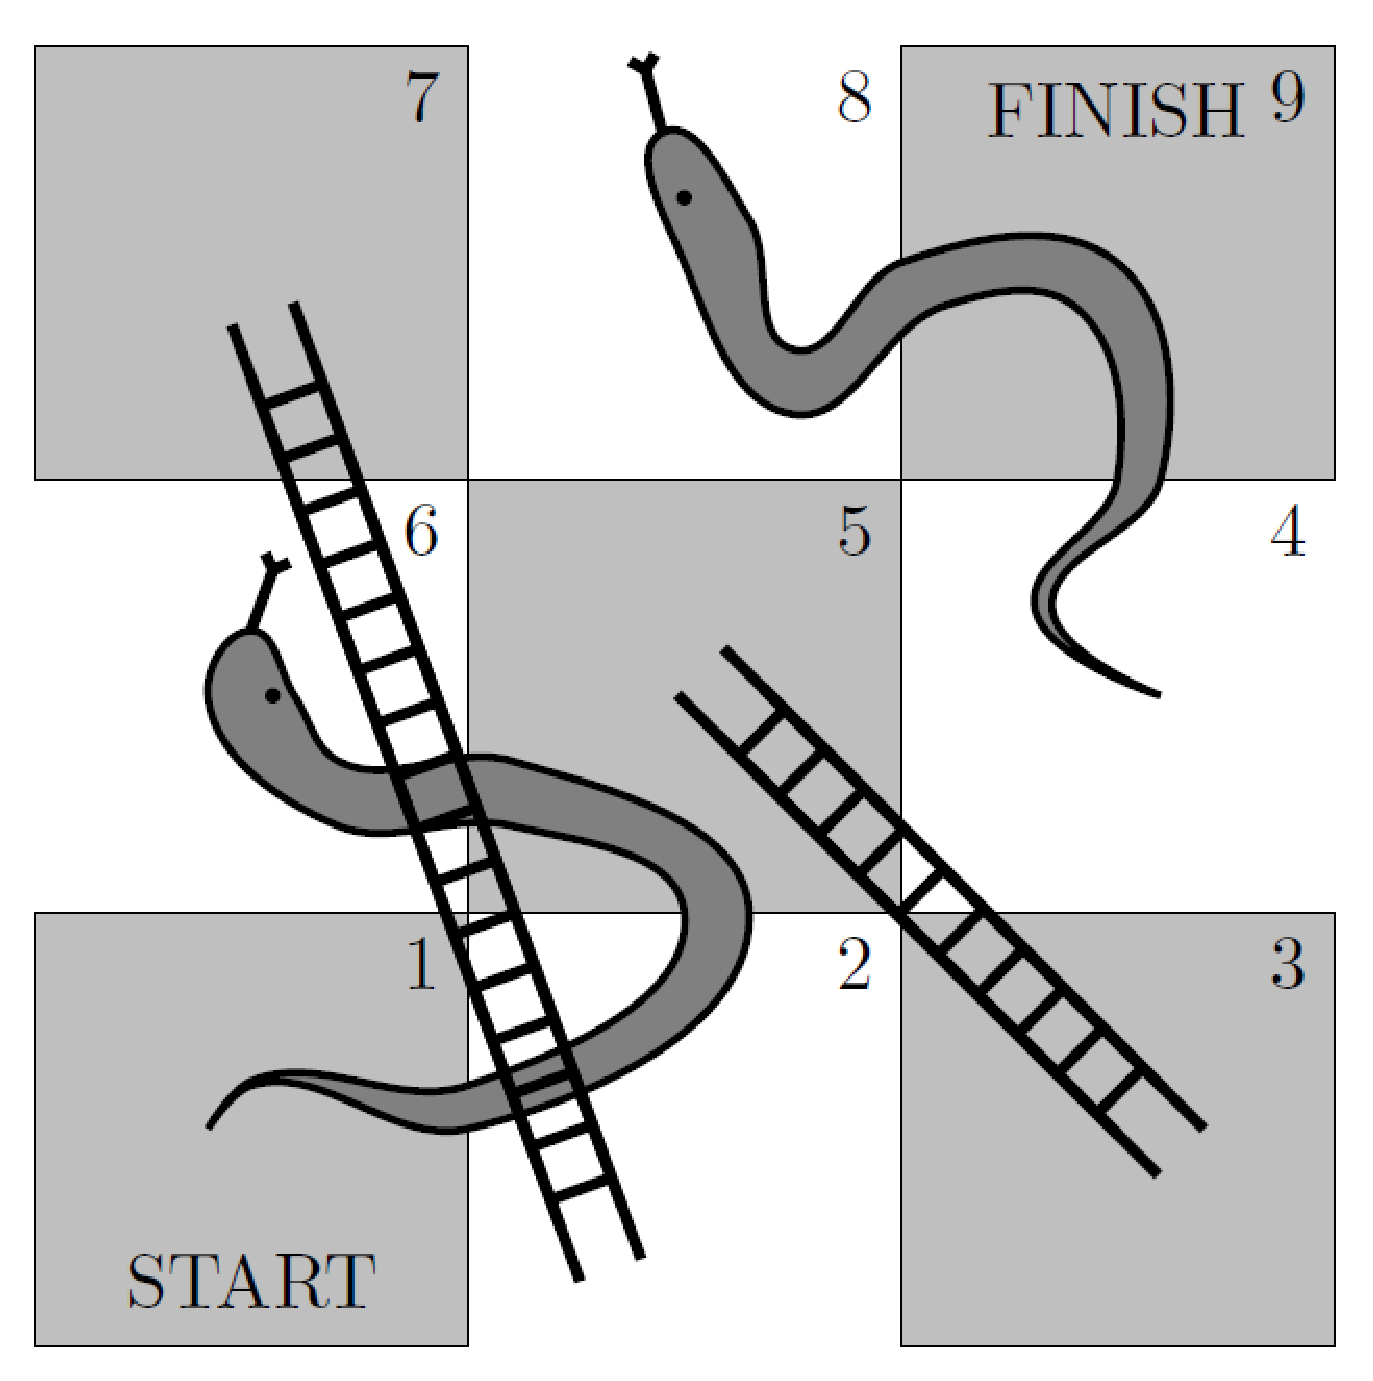
\includegraphics{Probability/Markov_chains/Markov_chains_1_1.eps}}
\end{figure}

At each turn a player tosses a fair coin and advances one or two places according to whether the coin lands heads or tails. If you land at the foot of a ladder you climb to the top, but if you land at the head of a snake you slide down to the tail. How many turn on average does it take to complete the game?

What is the probability that a player who has reached the middle square will complete the game without slipping back to square 1?
\end{problem}

\begin{solution}[\bf Solution.]
The transition matrix is
\be
\ba{c}
\ba{cccccc}
& \ 1 \ \ &\ 4 \ \ &\ 5\ \ &\ 7\ \ &\ 9\ \
\ea \\
\ba{c}
1 \\
4 \\
5 \\
7 \\
9
\ea
\lob
\ba{ccccc}
0 & 0 & \frac 12 & \frac 12 & 0 \\
\frac 12 & 0 & \frac 12 & 0 & 0 \\
\frac 12 & 0 & 0 & \frac 12 & 0  \\
0 & \frac 12 & 0 & 0 & \frac 12  \\
\ 0 \ \ & \ 0 \ \ & \ 0 \ \  &\  0 \ \  & \  1 \ \
\ea
\rob.
\ea
\ee

Let $k_i=\E_i(\text{time to hit 9})$ and $k_9=0$. We have
\be
\left\{\ba{l}
k_1 = 1 + \frac 12 k_7 + \frac 12 k_5\\
\\
k_4 = 1 + \frac 12 k_5 + \frac 12 k_1\\
\\
k_5 = 1 + \frac 12 k_1 + \frac 12 k_7\\
\\
k_7 = 1 + \frac 12 k_4 + \frac 12 k_9
\ea\right.\ \ra \
\left\{\ba{l}
k_1 = 1 + \frac 12 k_7 + \frac 12 k_5\\
\\
k_4 = 1 + \frac 12 k_5 + \frac 12 k_1\\
\\
k_5 = 1 + \frac 12 k_1 + \frac 12 k_7\\
\\
k_7 = 1 + \frac 12 k_4
\ea\right. \ \ra \
\left\{\ba{l}
k_1 = 7\\
\\
k_4 = 8\\
\\
k_5 = 7\\
\\
k_7 = 5
\ea\right.
\ee

Let $h_i=\pro_i(\text{hit 9 before 1})$ and $h_1=0, h_9=1$. We have
\be
\left\{\ba{l}
h_4 = \frac 12 h_5 + \frac 12 h_1\\
\\
h_5 = \frac 12 h_1 + \frac 12 h_7\\
\\
h_7 = \frac 12 h_4 + \frac 12 h_9
\ea\right.\ \ra \
\left\{\ba{l}
h_4 = \frac 12 h_5\\
\\
h_5 = \frac 12 h_7\\
\\
h_7 = \frac 12 h_4 + \frac 12
\ea\right. \ \ra \
\left\{\ba{l}
h_4 = \frac 17\\
\\
h_5 = \frac 27\\
\\
h_7 = \frac 47
\ea\right.
\ee

\end{solution}

\begin{problem}
Let $(X_n)_{n\geq 0}$ be a Markov chain on $\{0,1,\dots\}$ with transition probabilities given by
\be
p_{01}=1,\quad p_{ii+1}+p_{ii-1}=1, \quad p_{ii+1}=\lob\frac{i+1}{i}\rob^2p_{ii-1},\quad i\geq 1
\ee

Show that if $X_0=0$ the probability that $X_n\geq 1$ for all $n\geq 1$ is $6/\pi^2$.
\end{problem}

\begin{solution}[\bf Solution.]
Let $h_i=\pro_i(\text{hit 0})$ and $h_0=1$. We have
\be
h_{i} = p_{ii+1}h_{i+1} + p_{ii-1}h_{i-1}
\ee

so $u_{i} = h_{i-1}-h_i$ satisfies
\be
p_{ii+1}u_{i+1} = p_{ii-1}u_i \ \ra \ u_{i+1} = \lob \frac{p_{ii-1}}{p_{ii+1}}\rob u_i \ \ra \ u_{i+1} = \lob \frac{i}{i+1}\rob^2 u_i = \lob \frac{1}{i+1}\rob^2 u_1
\ee

Thus, we have
\be
h_i = h_0 - (h_0-h_i) = 1 - \sum^i_{k=1} u_k = 1-u_1\sum^i_{k=1}\frac 1{k^2}.
\ee

Since $(h_i:i\geq 0)$ is the minimal non-negative solution, $h_\infty=0$. so
\be
u_1=\lob\sum^\infty_{k=1}\frac 1{k^2}\rob^{-1} = \frac 6{\pi^2}\quad (\text{Basel problem})
\ee

Thus,
\be
\pro_0(X_n\geq 1,\ \forall n\geq 1) = 1- h_1 = \frac 6{\pi^2}.
\ee
\end{solution}

\begin{problem}
Let $(Y_n)_{n\geq 0}$ be independent identically distributed random with $\pro(Y_j=1)=\pro(Y_j=-1)=1/2$. Set $X_0=1$ and $X_n=X_0+Y_1+\dots+Y_n,\ n\geq 1$. Define the extinction time $H_0$ (the time of hitting 0) and find the probability generating function $\phi(s)=\E_1s^{H_0}$. Calculate the mean value $\E_1H_0$.

Suppose the distribution of $Y_j$ is changed to $\pro(Y_j=2)=\pro(Y_j=-1)=1/2$. Show that $\phi$ now satisfies
\be
s\phi^3-2\phi +s =0.
\ee
\end{problem}

\begin{solution}[\bf Solution.]
We know that the probability generating function of a sum of independent random variables is simply the product of the probability generating functions. Thus,
\be
\phi(s) = \E_1s^{H_0} = \frac 12\E_2s^{H_0+1} +\frac 12\E_0s^{H_0+1} = \frac s2\E_2s^{H_0}+\frac{s}{2}\E_0s^{H_0} = \frac s2 \phi^2(s) + \frac s2
\ee

So we have
\be
s\phi^2 - 2\phi + s = 0 \ \ra \ \phi(s) = \frac {2\pm\sqrt{4-4s^2}}{2s} = \frac {1\pm\sqrt{1-s^2}}s
\ee

Since $\phi(0)=0$, we choose
\be
\phi(s) = \frac {1-\sqrt{1-s^2}}s \ \ra \ \phi'(s) = \frac{s(-1/2)(-2s)(1-s^2)^{-1/2}- (1-\sqrt{1-s^2})}{s^2} = \frac {1-\sqrt{1-s^2}}{s^2\sqrt{1-s^2}}
\ee

Thus,
\be
\E_1H_0 = \lim_{s\to 1^-}\phi'(s) = \infty.
\ee

If $\pro(Y_j=2)=\pro(Y_j=-1)=1/2$, we have
\be
\phi(s) = \frac s2\E_3s^{H_0}+\frac s2\E_0s^{H_0} = \frac s2 \phi^3(s)+ \frac s2 \ \ra \ s\phi^3-2\phi +s =0
\ee
as required.
\end{solution}

\begin{problem}
A random sequence of non-negative integers $(F_n)_{n\geq 0}$ is obtained by setting $F_0=0$ and $F_1=1$ and, one $F_0,\dots,F_n$ are known, taking $F_{n+1}$ to be either the sum or the difference of $F_{n-1}$ and $F_n$, each with probability $1/2$. Is $(F_n)_{n\geq 0}$ a Markov chain? By considering the Markov chain $X_n=(F_{n-1},F_n)$, find the probability that $(F_n)_{n\geq 0}$ reaches 3 before first returning to 0.

Draw enough of the flow diagram for $(F_n)_{n\geq 0}$ to establish a general pattern. Hence, using the strong Markov property, show that the hitting probability for $(1,1)$, starting from $(1,2)$, is $(3-\sqrt{5})/2$. Deduce that $F_n\to \infty$ as $n\to \infty$.
\end{problem}

\begin{solution}[\bf Solution.]
$(F_n)$ is not a Markov chain, as $F_{n+1}$ depends on $F_n$ and $F_{n-1}$, but the pair $(F_{n-1},F_n)$ is.

\centertexdraw{

    \def\bdot {\fcir f:0 r:0.025 }

    \drawdim in

    \arrowheadtype t:F \arrowheadsize l:0.08 w:0.04
    \linewd 0.01 \setgray 0

    \move (1 0)\bdot
    \move (0 0)\bdot
    \move (0.5 0.5)\bdot
    \move (0.2 1)\bdot
    \move (0.8 1)\bdot
    \move (0 -0.5)\bdot
    \move (-0.3 -0.5)\bdot
    \move (0.3 -1)\bdot
    \move (0.0 -1)\bdot
    \move (-0.3 -1)\bdot
    \move (-0.6 -1)\bdot
    \move (1 -0.5)\bdot
    \move (1.3 -0.5)\bdot
    \move (1.3 -1)\bdot
    \move (1.6 -1)\bdot
    \move (1 -1)\bdot
    \move (0.7 -1)\bdot

    \move (0.9 0) \avec(0.5 0) \move(0.9 0) \lvec (0.1 0)
    \move (0.05 0.05) \avec(0.25 0.25) \move(0.05 0.05) \lvec (0.45 0.45)
    \move (0.55 0.45) \avec(0.75 0.25) \move(0.55 0.45) \lvec (0.95 0.05)
    \move (0.45 0.55) \avec(0.35 0.75) \move(0.45 0.55) \lvec (0.25 0.95)
    \move (0.25 1) \avec(0.5 1) \move(0.25 1) \lvec (0.75 1)
    \move (0.75 0.95) \avec(0.65 0.75) \move(0.75 0.95) \lvec (0.55 0.55)

    \move (0 -0.05) \avec(0 -0.25) \move(0 -0.05) \lvec (0 -0.45)
    \move (-0.05 -0.5) \avec(-0.2 -0.5) \move(-0.05 -0.5) \lvec (-0.25 -0.5)
    \move (-0.25 -0.45) \avec(-0.1 -0.15) \move(-0.25 -0.45) \lvec (-0.05 -0.05)

    \move (1.05 -0.05) \avec(1.15 -0.25) \move(1.05 -0.05) \lvec (1.25 -0.45)
    \move (1.25 -0.5) \avec(1.1 -0.5) \move(1.25 -0.5) \lvec (1.05 -0.5)
    \move (1 -0.45) \avec(1 -0.25) \move(1 -0.45) \lvec (1 -0.05)

    \move (-0.3 -0.55) \avec(-0.3 -0.75) \move(-0.3 -0.55) \lvec (-0.3 -0.95)
    \move (-0.35 -1) \avec(-0.5 -1) \move(-0.35 -1) \lvec (-0.55 -1)
    \move (-0.55 -0.95) \avec(-0.4 -0.65) \move(-0.55 -0.95) \lvec (-0.35 -0.55)

    \move (0.05 -0.55) \avec(0.15 -0.75) \move(0.05 -0.55) \lvec (0.25 -0.95)
    \move (0.25 -1) \avec(0.1 -1) \move(0.25 -1) \lvec (0.05 -1)
    \move (0 -0.95) \avec(0 -0.75) \move(0 -0.95) \lvec (0 -0.55)

    \move (1 -0.55) \avec(1 -0.75) \move(1 -0.55) \lvec (1 -0.95)
    \move (0.95 -1) \avec(0.8 -1) \move(0.95 -1) \lvec (0.75 -1)
    \move (0.75 -0.95) \avec(0.9 -0.65) \move(0.75 -0.95) \lvec (0.95 -0.55)

    \move (1.35 -0.55) \avec(1.45 -0.75) \move(1.35 -0.55) \lvec (1.55 -0.95)
    \move (1.55 -1) \avec(1.4 -1) \move(1.55 -1) \lvec (1.35 -1)
    \move (1.3 -0.95) \avec(1.3 -0.75) \move(1.3 -0.95) \lvec (1.3 -0.55)

    \htext (-0.35 -0.05){(2,1)}
    \htext (1.05 -0.05){(1,2)}
    \htext (0.1 0.45){(1,1)}
    \htext (-0.15 0.95){(1,0)}
    \htext (0.85 0.95){(0,1)}

    \htext (0.65 -0.55){(3,1)}
    \htext (1.35 -0.55){(2,3)}

    \htext (-0.65 -0.55){(3,2)}
    \htext (0.05 -0.55){(1,3)}

    \htext (-0.95 -1.05){(5,3)}
    \htext (1.65 -1.05){(3,5)}

    \htext (-0.5 -1.2){(2,5)}
    \htext (-0.15 -1.2){(4,1)}
    \htext (0.2 -1.2){(3,4)}

    \htext (0.55 -1.2){(4,3)}
    \htext (0.9 -1.2){(1,4)}
    \htext (1.25 -1.2){(5,2)}

\move (0 1.2)
\move (0 -1.3)
}

The initial part of the diagram shows that the level $F_n=3$ can be reached from $(F_0,F_1)=(0,1)$ either at (2,3) or (1,3). To hit this level before visiting level $F_n=0$ (i.e. (1,0)), we have two straight paths, supplemented with a number of adjacent triangular cycles. The two possibilities give the probability
\be
1\cdot \frac 12 \cdot \frac 12 \lob 1+ \frac 18 + \frac 1{8^2} + \cdots\rob = \frac 27,\quad 1\cdot \frac 12 \cdot \frac 12 \cdot \frac 12 \lob 1+ \frac 18 + \frac 1{8^2} + \cdots\rob = \frac 17,
\ee
which adds to 3/7.

One can see a triangular 'pattern' emerging from the diagram, with treelike symmetries. In particular, we define
\be
\left\{\ba{l}
p:=\pro_{(1,2)}(\text{hit (1,1)}) = \pro_{(2,3)}(\text{hit (1,2)}) = \pro_{(1,3)}(\text{hit (2,1)})\\
\\
p':=  \pro_{(2,1)}(\text{hit (1,1)}) = \pro_{(3,2)}(\text{hit (2,1)}) = \pro_{(3,1)}(\text{hit (1,2)})
\ea\right.
\ee

Conditioning on the first jump, by the strong Markov property, we can write
\be
\left\{\ba{l}
\pro_{(1,2)}(\text{hit (1,1)}) = \frac 12 \pro_{(2,3)}(\text{hit (1,1)}) + \frac 12 \pro_{(2,1)}(\text{hit (1,1)}) \\
\\
\pro_{(2,1)}(\text{hit (1,1)}) = \frac 12 \pro_{(1,3)}(\text{hit (1,1)}) + \frac 12
\ea\right.\ \ra \
\left\{\ba{l}
p = \frac 12 p^2 + \frac 12 p'\\
\\
p' = \frac 12 pp' + \frac 12
\ea\right.
\ee

Then we have
\be
(p-1)(p^2-3p+1)=0\ \ra \ p=1,(3\pm\sqrt{5})/2.
\ee

We are interested in the minimal non-negative root. Thus the probability should be $(3-\sqrt{5})/2$.

We know (1,1) is transient (because $p<1$), so the (only) communicating class is transient. Thus, we have
\be
\pro(X_n=(i,j) \text{ for infinitely many }n) = 0,\ \forall (i,j) \ \ra \ \pro(F_n=i \text{ for infinitely many }n) = 0,\ \forall i
\ee

Suppose that $F_n\nrightarrow\infty$ as $n\to \infty$. Thus $\exists K:\forall N\in\N$, $\exists n\geq N$ s.t. $F_n\leq K$ for infinitely many $n$. Thus, $\exists i\leq K: F_n=j$ for infinitely many $n$ and
\be
\pro(F_n=i \text{ for infinitely many }n) = 0\ \ra \ \pro(F_n\nrightarrow \infty) = 0 \ \ra \ \pro(F_n\to \infty) = 1.
\ee

Now we consider more general case: taking the sum with $q$ and taking the difference with $1-q$. Thus, we have
\be
\left\{\ba{l}
\pro_{(1,2)}(\text{hit (1,1)}) = q \pro_{(2,3)}(\text{hit (1,1)}) + (1-q) \pro_{(2,1)}(\text{hit (1,1)}) \\
\\
\pro_{(2,1)}(\text{hit (1,1)}) = q \pro_{(1,3)}(\text{hit (1,1)}) + 1-q
\ea\right.\ \ra \
\left\{\ba{l}
p = q p^2 + (1-q) p'\\
\\
p' = q pp' + (1-q)
\ea\right.
\ee
Then we have (if $0<q\leq 1$)
\be
(p-1)(q^2p^2-q(2-q)p+(1-q)^2)=0\ \ra \ p=1,\frac {2-q\pm\sqrt{4q-3q^2}}{2q}.
\ee

We see that $\frac {2-q-\sqrt{4q-3q^2}}{2q}>0$ and we take it as the minimal non-negative root if
\be
\frac {2-q -\sqrt{4q-3q^2}}{2q}<1 \ \ra \ q>\frac 13
\ee
otherwise, we take 1 as the minimal non-negative root. In other case $q=0$, it is easy to see that $p=1$. Thus,
\be
\left\{\ba{cl}
\frac {2-q-\sqrt{4q-3q^2}}{2q} \quad\quad & q>\frac 13\\
\\
1 & q \leq \frac 13
\ea\right.
\ee

\end{solution}

\begin{problem}
The rooted binary tree is an infinite graph $T$ with one distinguished vertex $R$ from which comes a single edge; at every other vertex there are three edges and there are no closed loops. The random walk on $T$ jumps from a vertex along each available edge with equal probability. Show that the random walk is transient.
\end{problem}

\begin{solution}[\bf Solution.]
Let $(X_n)_{n\geq 0}$ be the distance (the length of the shortest path) from $R$. Then $(X_n)_{n\geq 0}$ is a Markov chain on $\N_0$ with transition probabilities $p_{i,i+1} = \frac 23$ and $p_{i,i+1} = \frac 13$.

Let $h_i = \pro_i(\text{hit } 0)$. We have the recurrence relation
\be
h_i = \frac 13 h_{i-1} + \frac 23 h_{i+1}
\ee
for $i \geq 1$ with boundary condition $h_0 = 1$. The minimal non-negative solution to this recurrence relation is $h_i = \bb{\frac 12 }^i$. Since $h_1 = \pro_R(\text{return to }R) < 1$, the random walk is transient.

%To show the random walk on $T$ is transient, we only need to show that $R$ is transient since the Markov chain is irreducible (with only one communicating %class). For $R$, it is sufficient to show either of the following two statements
%\be
%\left\{
%\ba{l}
%f_{R} = \pro_R(T_R<+\infty) = \pro_R(\text{return to }R) < 1\\
%\\
%\sum_{n\geq 0}p_{RR}^{(n)} < \infty
%\ea\right.
%\ee
%
%\centertexdraw{
%
%    \def\bdot {\fcir f:0 r:0.025 }
%
%   \drawdim in
%
%    \arrowheadtype t:F \arrowheadsize l:0.08 w:0.04
%    \linewd 0.01 \setgray 0
%
%    \move (0 0)\bdot
%    \move (0.5 0)\bdot
%    \move (1 0.5)\bdot
%    \move (1 -0.5)\bdot
%    \move (1.5 0.75)\bdot
%    \move (1.5 0.25)\bdot
%    \move (1.5 -0.75)\bdot
%    \move (1.5 -0.25)\bdot
%
%    \move (0.05 0) \avec(0.2 0) \move(0.45 0) \avec(0.3 0) \move(0.05 0) \lvec (0.45 0)
%    \move (0.55 0.05) \avec(0.7 0.2) \move (0.95 0.45) \avec(0.8 0.3) \move(0.55 0.05) \lvec (0.95 0.45)
%    \move (0.55 -0.05) \avec(0.7 -0.2) \move (0.95 -0.45) \avec(0.8 -0.3) \move(0.55 -0.05) \lvec (0.95 -0.45)
%
%    \move (1.04 0.52) \avec(1.22 0.61) \move (1.46 0.73) \avec(1.28 0.64) \move(1.04 0.52) \lvec (1.46 0.73)
%    \move (1.04 0.48) \avec(1.22 0.39) \move (1.46 0.27) \avec(1.28 0.36) \move(1.04 0.48) \lvec (1.46 0.27)
%    \move (1.04 -0.52) \avec(1.22 -0.61) \move (1.46 -0.73) \avec(1.28 -0.64) \move(1.04 -0.52) \lvec (1.46 -0.73)
%    \move (1.04 -0.48) \avec(1.22 -0.39) \move (1.46 -0.27) \avec(1.28 -0.36) \move(1.04 -0.48) \lvec (1.46 -0.27)
%
%    \htext (-0.2 0){$R$}
%    \htext (0.4 -0.15){1}
%    \htext (0.95 -0.65){2}
%    \htext (0.95 0.3){3}
%
%    \htext (0.1 0.08){1}
%    \htext (0.3 0.05){1/3}
%    \htext (0.6 0.35){1/3}
%    \htext (0.6 -0.5){1/3}
%
%}
%
%{\flushleft \emph{Approach 1}}. From the above diagram, we know that
%\be
%f_R = \pro_R(T_R<+\infty) = \pro_R(\text{return to }R) = h_R^R = h_1^R = h_2^1=h_3^1 \ \ra \ h_1^R = \frac 13 + \frac 13 h_2^R + \frac 13 h_3^R
%\ee
%
%Thus, we have
%\be
%f_R = \frac 13 + \frac 23 f_R^2 \ \ra \ f_R=1,\frac 12
%\ee
%
%So we have $f_R<1$ as we take the minimal non-negative $f_R=\frac 12$.
%
%{\flushleft \emph{Approach 2}}. Let $X_n$ be the distance from $R$. Then $(X_n)_{n\geq 0}$ is a biased random walk on \{0,1,2,\dots\} with $p_{ii+1}=2/3$, %$p_{ii-1}=1/3$. Since the random walk can only return to $R$ in an even number of jumps, we have
%\be
%p_{RR}^{(2n)} = p_{00}^{(2n)} = \binom{2n}{n}\lob\frac 13\rob^n \lob\frac 23\rob^n,\quad n\geq 0
%\ee
%
%With Stirling formula $n!\sim \sqrt{2\pi n}(n/e)^n$, we have
%\be
%p_{00}^{(2n)} = \frac{(2n)!}{n!n!}(8/9)^n \sim \frac{(8/9)^n}{\sqrt{n\pi}},\quad n\to\infty
%\ee
%
%Choose a large enough $N<\infty$, we have
%\beast
%\sum_{n\geq 0}p_{00}^{(2n)} & = & \sum^{N-1}_{n=0}p_{00}^{(2n)} + \sum^\infty_{n=N}p_{00}^{(2n)} < \sum^{N-1}_{n=0}1 + \sum^\infty_{n=N}p_{00}^{(2n)} = N + \sum^\infty_{n=N}p_{00}^{(2n)} \\%
%& \sim & N + \sum^\infty_{n=N}\frac{(8/9)^n}{\sqrt{n\pi}} < N + \frac 1{\sqrt{N\pi}}\sum^\infty_{n=N}(8/9)^n = N + \frac 9{\sqrt{N\pi}}\lob\frac 89\rob^N < \infty
%\eeast
%as required.

\end{solution}

\begin{problem}
Let $(X_n)_{n\geq 0}$ be a Markov chain on $\{0,1,\dots\}$ with transition probabilities given by
\be
p_{01}=1,\quad p_{ii+1}+p_{ii-1}=1, \quad p_{ii+1}=\lob\frac{i+1}{i}\rob^\alpha p_{ii-1},\quad i\geq 1,\ \alpha \in(0,\infty)
\ee

What is the value of $\pro(X_n\to\infty\text{ as }n\to\infty)$?
\end{problem}

\begin{solution}[\bf Solution.]
Let $h_i=\pro_i(\text{hit 0})$ and $h_0=1$. We have
\be
h_{i} = p_{ii+1}h_{i+1} + p_{ii-1}h_{i-1}
\ee

so $u_{i} = h_{i-1}-h_i$ satisfies
\be
p_{ii+1}u_{i+1} = p_{ii-1}u_i \ \ra \ u_{i+1} = \lob \frac{p_{ii-1}}{p_{ii+1}}\rob u_i \ \ra \ u_{i+1} = \lob \frac{i}{i+1}\rob^\alpha u_i = \lob \frac{1}{i+1}\rob^\alpha u_1
\ee

Thus, we have
\be
h_i = h_0 - (h_0-h_i) = 1 - \sum^i_{k=1} u_k = 1-u_1\sum^i_{k=1}\frac 1{k^\alpha}.
\ee

Since $(h_i:i\geq 0)$ is the minimal non-negative solution, $h_\infty=0$. so
\be
u_1=\lob\sum^\infty_{k=1}\frac 1{k^\alpha}\rob^{-1} \ \ra \ h_i = 1-\left.\sum^i_{k=1}\frac 1{k^\alpha}\right/\sum^\infty_{k=1}\frac 1{k^\alpha}.
\ee

Thus,
\be
h_i=\left\{\ba{ll}
=1 \quad\quad & \text{if } \sum^\infty_{k=1}\frac 1{k^\alpha} =\infty \ (\alpha\leq 1)\\
\\
<1 & \text{if } \sum^\infty_{k=1}\frac 1{k^\alpha} < \infty \ (\alpha >  1)
\ea\right.\ \ra \
(X_n)_{n\geq 0} \text{ is }\left\{
\ba{l}
\text{recurrent if }\alpha\leq 1\\
\text{transient if }\alpha > 1
\ea\right.
\ee

Equivalently,
\be
\pro(X_n\to\infty\text{ as }n\to\infty)
=\left\{\ba{ll}
0 \quad\quad & \text{if } \alpha\leq 1\\
1 & \text{if } \alpha >  1
\ea\right.
\ee
\end{solution}

\begin{problem}
Show that the simple symmetric random walk in $\Z^4$ is transient.
\end{problem}

\begin{solution}[\bf Solution.]
We project the random walk $(X_n^d)$ on $\Z^d$ to three dimensions by discarding all coordinates but the first three. The project chain $(X_n^{\text{proj}})$ on $\Z^3$ stays where it is with probability $(d-3)/d$, but when it jumps, it behaves as the nearest-neighbour symmetric walk in dimension 3.

Let $(X_n)_{n\geq 0}$ be the simple symmetric random walk in $\Z^4$ with
\be
p_{ij}=\left\{
\ba{ll}
1/8 \quad \quad &\text{if }|i-j|=1\\
0 & \text{otherwise}
\ea
\right.\quad\quad i,j\in\Z^4
\ee

Let $(Y_m)_{m\geq 0}$ be the projection of $(X_n)_{n\geq 0}$ on $\Z^3$ with
\be
\tilde{p}_{ij}=\left\{
\ba{ll}
1/4  & \text{if }|i-j|=0 \\
1/8 \quad \quad &\text{if }|i-j|=1\\
0 & \text{otherwise}
\ea
\right. \quad\quad i,j\in\Z^3
\ee

Observe $(Y_{m})_{m\geq 0}$ only when it moves, the resulting process $(Z_t)_{t\geq 0}$ is given by $Z_t=Y_{S_t}$ where $S_0=0$ and
\be
S_{t+1} = \inf\{m\geq S_t: Y_m \neq Y_{S_t}\}
\ee
so $S_t$ is a stopping time and by strong Markov property
\beast
& & \pro(Z_{t+1}=i_{t+1}|Z_0=i_0,\dots,Z_t=i_t) \\
& = & \pro(Y_{S_{t+1}}=i_{t+1}|Y_{S_0}=i_0,\dots,Y_{S_t}=i_t) = \pro_{i_t}(Y_{S_1}=i_{t+1}) \quad (\text{since $Y$ is Markov chain})\\
& = & \hat{p}_{i_ti_{t+1}}
\eeast
so $Z$ is Markov chain with transition matrix $\hat{P}$ where $\hat{p}_{ii}=0$ and for $i\neq j$
\be
\hat{p}_{ij} = \frac{\tilde{p}_{ij}}{\sum_{k\neq i}\tilde{p}_{ik}}
\ee
so we have
\be
p_{ij}=\left\{
\ba{ll}
1/6 \quad \quad &\text{if }|i-j|=1\\
0 & \text{otherwise}
\ea
\right.\quad\quad i,j\in\Z^4
\ee
thus $(Z_t)_{t\geq 0}$ is the simple symmetric random walk in $\Z^3$. We know $(Z_t)_{t\geq 0}$ is transient, so $\sum_{n\geq 0}\hat{p}_{ii}^{(n)}<\infty$. Also, we have $p_ii^{(n)}< \tilde{p}_ii^{(n)}<\hat{p}_ii^{(n)}$. Hence,
\be
\sum_{n\geq 0}p_{ii}^{(n)}< \sum_{n\geq 0}\tilde{p}_{ii}^{(n)}<\sum_{n\geq 0}\hat{p}_{ii}^{(n)}<\infty
\ee
\end{solution}

\begin{problem}
Find all invariant distributions of the transition matrix
\be
P=
\lob
\ba{ccccc}
\frac 12 & 0 & 0 & 0 & \frac 12 \\
0 & \frac 12 & 0 & \frac 12 & 0 \\
0 & 0 &  1 & 0 & 0  \\
0 & \frac 14 &  \frac 14 & \frac 14 & \frac 14  \\
\ \frac 12 \ \  & \ 0 \ \ & \ 0 \ \  &\  0 \ \  &  \ \frac 12 \ \
\ea
\rob.
\ee
\end{problem}

\begin{solution}[\bf Solution.]
We have
\be
\pi P = \pi \ \ra \ \pi = \lob\frac 12 p,0,1-p,0,\frac 12 p\rob,\quad 0\leq p\leq 1
\ee

This is not unique. This example shows that the non-uniqueness occurs when the matrix is not irreducible.
\end{solution}

\begin{problem}
Gas molecules move about randomly in a box which is divided into two halves symmetrically by a partition. A hole is made in the partition. Suppose there are $N$ molecules in the box. Show that the number of molecules on the side of the partition just after a molecule has passed through the hole evolves as a Markov chain. What are the transition probabilities? What is the invariant distribution of this chain?
\end{problem}

\begin{solution}[\bf Solution.]
The state-space is \{0,1,\dots,N\} and the transition probabilities are
\be
p_{i,i+1} + p_{i,i-1} = 1, \quad p_{i,i-1} = \frac iN,\ i=1,\dots,N
\ee

Since the Markov chain is reversible, $P$ and $\pi$ are in detailed balance, i.e.
\be
\pi_ip_{i,i-1} = \pi_{i-1}p_{i-1,i} \ \ra \ \pi_i = \frac{p_{i-1,i}}{p_{i,i-1}}\pi_{i-1} = \frac{1-\frac {i-1}N}{\frac iN}\pi_{i-1} =\frac{N-i+1}{i}\pi_{i-1} = \binom{N}{i}\pi_0
\ee

Then we have
\be
1 = \sum^N_{i=0}\pi_i = \sum^N_{i=1}\binom{N}{i}\pi_0 = \pi_02^N \ \ra \ \pi_0=\lob\frac 12\rob^N \ \ra \ \pi_i = \binom{N}{i}\lob\frac 12\rob^N \ \ra \ \pi_i \sim \text{Bin}\lob N,\frac 12\rob.
\ee

\end{solution}

\begin{problem}
A particle moves on the eight vertices of a cube in the following way: at each step the particle is equally likely to move to each of the three adjacent vertices, independently of its past motion. Let $i$ be the initial vertex occupied by the particle, $o$ the vertex opposite $i$. Calculate each of the following quantities:

(i) the expected number of steps until the particle returns to $i$;

(ii) the expected number of visits to $o$ until the first return to $i$;

(iii) the expected number of steps until the first visit to $o$.
\end{problem}

\begin{solution}[\bf Solution.]
Draw the diagram
\centertexdraw{

    \def\bdot {\fcir f:0 r:0.025 }

    \drawdim in

    \arrowheadtype t:F \arrowheadsize l:0.08 w:0.04
    \linewd 0.01 \setgray 0

    \move (0 0)\bdot
    \move (1 0)\bdot
    \move (0 1)\bdot
    \move (1 1)\bdot
    \move (0.5 0.3)\bdot
    \move (1.5 0.3)\bdot
    \move (0.5 1.3)\bdot
    \move (1.5 1.3)\bdot

    \move (0 0) \lvec (1 0) \lvec(1 1) \lvec(0 1) \lvec(0 0)
    \move (0 1) \lvec(0.5 1.3) \lvec(1.5 1.3) \lvec(1 1)
    \move (1 0) \lvec(1.5 0.3) \lvec(1.5 1.3)

    \linewd 0.01 \lpatt(0.067 0.1)

    \move (0 0) \lvec (0.5 0.3) \lvec (0.5 1.3) \move(0.5 0.3) \lvec(1.5 0.3)

    \htext (-0.1 1.05){1}
    \htext (0.9 1.05){2}
    \htext (-0.1 -0.15){3}
    \htext (0.9 -0.15){4}

    \htext (0.4 1.35){5}
    \htext (1.4 1.35){6}
    \htext (0.35 0.3){7}
    \htext (1.55 0.25){8}

}
We take 1 as $i$ and 8 as $o$ and the transition probabilities are given by
\be
p_{ij}=\left\{
\ba{ll}
1/3 \quad \quad &\text{if $i$ and $j$ are connected}\\
0 & \text{otherwise}
\ea
\right.\quad\quad
\ee

Thus the equilibrium distribution is $\pi = (\frac 18, \frac 18,\frac 18,\frac 18,\frac 18,\frac 18,\frac 18,\frac 18)$.

(i) Since the Markov chain is irreducible and positive recurrent, we have
\be
m_k = \E_kT_k = \frac 1{\pi_k}\ \ra \ m_1 = \frac 1{\pi_1} = 8.
\ee

(ii) With the same condition, we have $\forall j\neq k$
\be
\E_k(\text{number of visits to $j$ before returning to $k$}) = \frac {\pi_j}{\pi_k} = 1.
\ee

(iii) We see that 2, 3, 5 are symmetric as well as 4, 6, 7. Thus we have 4-state Markov chain \{I(1), II(2,3,5), III(4,6,7), IV(8)\} and let $k_i=\E_i(\text{time to hit 8})$. We have $k_{IV}=0$ and
\be
\left\{
\ba{l}
k_I = 1 + k_{II} \\
\\
k_{II} = 1 + \frac 13k_I + \frac 23 k_{III}\\
\\
k_{III} = 1 + \frac 13k_{IV} + \frac 23k_{II}
\ea\right. \ \ra \
k_I = 10,\ k_{II} = 9, \ k_{III} = 7.
\ee

Thus, the answer is 10.
\end{solution}

\begin{problem}
Let $(X_n)_{n\geq 0}$ be a Markov chain on $\{1,2,3\}$ with transition matrix
\be
\lob
\ba{ccc}
0 & 1 & 0 \\
0 & \frac 23 & \frac 13 \\
p &  \quad 1-p\quad \quad & 0
\ea
\rob.
\ee

Find the invariant distributions of the transition matries when (a) $p=\frac{1}{16}$,  (b)  $p=\frac{1}{6}$, (c)  $p=\frac{1}{12}$. (in Example Sheet 1)
\end{problem}

\begin{solution}[\bf Solution.]
With the definition of invariant distribution, we have
\be
\pi
\lob
\ba{ccc}
0 & 1 & 0 \\
0 & \frac 23 & \frac 13 \\
p &  \quad 1-p\quad \quad & 0
\ea
\rob = \pi \ \ra \ \pi = \frac 1{p+4}(p,3,1) \ \ra \ \pi_1=\lim_{n\to\infty}\pro(X_n=1|X_0=1)=\frac p{p+4}.
\ee

Check the results in Example 1 we have

(a) $p=\frac 1{16}\ \ra \ \pi_1 = \frac{1/16}{1/16+4} = \frac 1{65} = \lim_{n\to\infty}p_{11}^{(n)} = \lim_{n\to\infty}\frac 1{65} -\frac 25\lob-\frac 14\rob^n + \frac {18}{13} \lob -\frac{1}{12}\rob^n$.

(b) $p=\frac 1{6}\ \ra \ \pi_1 = \frac{1/6}{1/6+4} = \frac 1{25} = \lim_{n\to\infty}p_{11}^{(n)} = \lim_{n\to\infty}\frac 1{25} + \lob \frac 1{3\sqrt{2}}\rob^n \lob \frac {24}{25}\cos\frac{3n\pi}4 +\frac {18}{25}\sin\frac{3n\pi}4\rob$.

(c) $p=\frac 1{12}\ \ra \ \pi_1 = \frac{1/12}{1/12+4} = \frac 1{49} = \lim_{n\to\infty}p_{11}^{(n)} = \lim_{n\to\infty}\frac 1{49} + \lob\frac {48}{49}-\frac {6}{7}n\rob\lob-\frac 1{6}\rob^n$.
\end{solution}

\begin{problem}
A fair die is thrown repeatedly. Let $X_n$ denote the sum of the first $n$ throws. Find
\be
\lim_{n\to\infty}\pro(X_n\text{ is a multiple of 13}).
\ee
\end{problem}

\begin{solution}[\bf Solution.]
Let $(X_n)_{n\geq 0}$ denote the sum of the first $n$ throws and $Y_n=X_n\bmod 13$. Thus, the its transition probabilities are given by
\be
p_{ij} = 1/6, \quad \text{for }j=(i+k)\bmod 13, \ k=1,2,3,4,5,6
\ee

Obviously, $P$ is irreducible. Also, we have $p_{00}^{(2)}>0$, $p_{00}^{(3)}>0$ and gcd(2,3)=1. Thus, we can see that state 0 is aperiodic (with the conclusion that state $i$ is aperiodic if and only if the set $\{n\geq 0:p_{ii}^{(n)}>0\}$ has no common divisor other than 1). So the irreducibility and aperiodicity imply that
\be
p_{ij}^{(n)}\to \pi_j,\quad \quad \text{as }n\to \infty
\ee

By symmetry, $\pi_i=1/13,\ \forall i$. Hence,
\be
\lim_{n\to\infty}\pro(X_n\text{ is a multiple of 13}) = \lim_{n\to\infty}\pro(Y_n=0) = \lim_{n\to\infty}p_{i0} = \pi_0 = \frac 1{13}.
\ee
\end{solution}

\begin{problem}
Each morning a student takes one of the three books she owns from her shelf. The probability that she chooses book $i$ is $\alpha_i$, $0<\alpha_i<1,\ i=1,2,3$, and choices on successive days are independent. In the evening she replaces the book at the left-hand end of the shelf. If $p_n$ denotes the probability that on day $n$ the student finds the books in the order 1,2,3, from left to right, show that, irrespective of the initial arrangement of the books, $p_n$ converges as $n\to \infty$, and determine the limit.
\end{problem}

\begin{solution}[\bf Solution.]
First we draw the diagram and Set 6-state Markov chain 1(123), 2(132), 3(213), 4(231), 5(312), 6(321).

\centertexdraw{

%\def\bdot {\fcir f:0 r:0.025 }

\drawdim in
\arrowheadtype t:F \arrowheadsize l:0.08 w:0.04
\linewd 0.01 \setgray 0

\move (0 0)\lcir r:0.15
\htext (-0.1 -0.05) {123}
\move (1 0)\lcir r:0.15
\htext (0.9 -0.05) {231}
\move (2 0)\lcir r:0.15
\htext (1.9 -0.05) {312}

\move (0 -0.8)\lcir r:0.15
\htext (-0.1 -0.85) {213}
\move (1 -0.8)\lcir r:0.15
\htext (0.9 -0.85) {321}
\move (2 -0.8)\lcir r:0.15
\htext (1.9 -0.85) {132}

\move (-0.05 -0.2) \avec(-0.05 -0.6)
\move (0.05 -0.6) \avec(0.05 -0.2)
\move (0.95 -0.2) \avec(0.95 -0.6)
\move (1.05 -0.6) \avec(1.05 -0.2)
\move (1.95 -0.2) \avec(1.95 -0.6)
\move (2.05 -0.6) \avec(2.05 -0.2)

\move (0.8 0) \avec(0.2 0)
\move (1.8 0) \avec(1.2 0)

\move (0.2 -0.8) \avec(0.8 -0.8)
\move (1.2 -0.8) \avec(1.8 -0.8)

\move (-0.15 0.15) \larc r:0.1 sd:0 ed:270
\move (-0.215 0.225) \avec(-0.225 0.215)
\move (1 0.2) \larc r:0.1 sd:-45 ed:225
\move (1.005 0.3) \avec(0.995 0.3)
\move (2.15 0.15) \larc r:0.1 sd:-90 ed:180
\move (2.225 0.215) \avec(2.215 0.225)

\move (-0.15 -0.95) \larc r:0.1 sd:90 ed:360
\move (-0.215 -1.025) \avec(-0.225 -1.015)
\move (1 -1) \larc r:0.1 sd:135 ed:45
\move (1.005 -1.1) \avec(0.995 -1.1)
\move (2.15 -0.95) \larc r:0.1 sd:180 ed:450
\move (2.225 -1.015) \avec(2.215 -1.025)

\move (1 -1) \larc r:1.45 sd:55 ed:125
\move (0.995 0.45) \avec(1.005 0.45)

\move (1 0.2) \larc r:1.45 sd:235 ed:305
\move (1.005 -1.25) \avec(0.995 -1.25)

\htext (-0.25 -0.4){$\alpha_2$}
\htext (0.1 -0.4){$\alpha_1$}
\htext (0.75 -0.4){$\alpha_3$}
\htext (1.1 -0.4){$\alpha_2$}
\htext (1.75 -0.4){$\alpha_1$}
\htext (2.1 -0.4){$\alpha_3$}

\htext (0.5 0.05){$\alpha_1$}
\htext (1.5 0.05){$\alpha_2$}
\htext (0.5 -0.95){$\alpha_3$}
\htext (1.5 -0.95){$\alpha_1$}

\htext (-0.4 0.1){$\alpha_1$}
\htext (1.15 0.2){$\alpha_2$}
\htext (2.3 0.1){$\alpha_3$}
\htext (-0.4 -0.9){$\alpha_2$}
\htext (1.15 -1){$\alpha_3$}
\htext (2.3 -0.9){$\alpha_1$}

\htext (1 0.5){$\alpha_3$}
\htext (1 -1.4){$\alpha_2$}

\htext (3 -0.6){$P=\lob\ba{cccccc}
\alpha_1 & 0 & \alpha_2 & 0 & \alpha_3 & 0 \\
0 & \alpha_1 & \alpha_2 & 0 & \alpha_3 & 0 \\
\alpha_1 & 0 & \alpha_2 & 0 & 0 & \alpha_3 \\
\alpha_1 & 0 & 0 & \alpha_2 & 0 & \alpha_3 \\
0 & \alpha_1 & 0 & \alpha_2 & \alpha_3 & 0 \\
\ 0\ \ & \ \alpha_1 \ \ &\ 0\ \ &\ \alpha_2\ \ &\ 0\ \ &\ \alpha_3\ \ \\
\ea\rob$}

\move (6 0)
}

Obviously, the Markov chain is irreducible. It is also aperiodic since
\be
\left\{
\ba{ll}
123\to 312\to 231 \to 123&\text{3 steps} \\
123\to 213\to 321 \to 231 \to 123 \quad\quad &\text{4 steps}
\ea\right.\
\ee

Therefore, $p_n=p_{i1}\to \pi_1,\ \forall i$. With the definition of invariant distribution. we see that
\be
\left\{
\ba{l}
\pi_1 = \alpha_1(\pi_1+\pi_3+\pi_4) \\
\pi_2 = \alpha_1(\pi_2+\pi_5+\pi_6)
\ea\right.\ \ra \
\pi_1+\pi_2 =\alpha_1.
\ee

Similarly, we have $\pi_3+\pi_4 = \alpha_2$ and substitute it into $\pi_1 = \alpha_1(\pi_1+\pi_3+\pi_4)$
\be
\pi_1 = \alpha_1(\pi_1+\alpha_2) \ \ra \ \pi_1 = \frac {\alpha_1\alpha_2}{1-\alpha_1}.
\ee
\end{solution}

\begin{problem}
In each of the following cases determine whether the stochastic matrix $P$ is reversible:
\begin{align*}
& (a)\quad \lob
\ba{cc}
p & 1-p\\
q & \ 1-q \ \
\ea\rob
;\quad\quad\quad\quad
(b)\quad \lob
\ba{ccc}
0 & p & 1-p\\
1-p & 0 & p \\
p& 1-p & 0
\ea\rob;\\
& (c)\quad I=\{0,1,\dots, N\} \text{ and } p_{ij}=0\text{ if }|j-i|\geq 2; \\
& (d)\quad I=\{0,1,\dots, N\} \text{ and } p_{01} = 1,\ p_{ii+1}=p,\ p_{ii-1}=1-p \text{ for }i\geq 1. \quad\quad\quad\quad\quad\quad\quad\quad\quad\quad\quad\quad\quad\quad\quad\quad\quad\quad
\end{align*}


\end{problem}

\begin{solution}[\bf Solution.]
If there exists $\pi$ s.t.
\be
\pi_ip_{ij} = \pi_jp_{ji},\quad \forall i,j\in I
\ee
then $P$ is reversible.

(a) We have
\be
\pi_1p_{12} = \pi_2p_{21}\ \ra\ \pi_1(1-p)=\pi_2q \ \ra \ \pi_1=\frac q{1-p+q},\ \pi_2=\frac{1-p}{1-p+q}\ \ra \ P \text{ is reversible}.
\ee

(b)
\be
\left\{
\ba{l}
\pi_1p_{12} = \pi_2p_{21}\\
\pi_1p_{13} = \pi_3p_{31}\\
\pi_2p_{23} = \pi_3p_{32}
\ea\right.\ \ra \
\left\{
\ba{l}
\pi_2 = \frac{p^2}{(1-p)^2}\pi_3\\
\pi_2 = \frac{1-p}p\pi_3
\ea\right.\ \ra \ p^3 = (1-p)^3 \ \ra \ p=\frac 12 \ \ra \ P \text{ is reversible iff }p=\frac 12.
\ee

(c)
\be
\left\{\ba{l}
\pi_ip_{i,i+1} = \pi_{i+1}p_{i+1,i} \\
\quad \quad \ \ra \ \pi_{i+1}=\frac{p_{i,i+1}}{p_{i+1,i}}\pi_i = \lob\prod^i_{k=0}\frac{p_{k,k+1}}{p_{k+1,k}}\rob\pi_0 \\
\sum^N_{i=0}\pi_i=1
\ea \right.\ \ra \
\pi_i = \frac{\prod^{i-1}_{k=0}\frac{p_{k,k+1}}{p_{k+1,k}}}{1+\sum^N_{i=1}\lob\prod^{i-1}_{k=0}\frac{p_{k,k+1}}{p_{k+1,k}}\rob} \ \ra \ P \text{ is reversible}.
\ee

(d)
\be
\left\{\ba{l}
\pi_0p_{01} = \pi_1p_{10} \ \ra \ \pi_0=(1-p)\pi_1\\
\pi_ip_{i,i+1} = \pi_{i+1}p_{i+1,i},\ i\geq 1\\
\quad \quad \ \ra \ \pi_{i+1}=\frac{p}{1-p}\pi_i = \frac 1p\lob\frac{p}{1-p}\rob^{i+1}\pi_0 \\
\sum^\infty_{i=0}\pi_i=1
\ea \right.\ \ra \
\pi_i = \frac{\lob\frac{p}{1-p}\rob^{i}}{p+\sum^\infty_{i=1}\lob\frac{p}{1-p}\rob^i} \ \ra \ P \text{ is reversible iff }p<\frac 12.
\ee

\end{solution}

\begin{problem}
A professor has $N$ umbrellas, which he keeps either at home or in his office. He walks to and from his office each day, and takes an umbrella with him if and only if it is raining. Throughout each journey, it either rains, with probability $p$, or remains fine, with probability $1-p$, independently of the past weather. What is the long run proportion of journeys on which he gets wet?
\end{problem}

\begin{solution}[\bf Solution.]
Let $X_n$ be the number of umbrellas at the start of journey $n$, then $(X_n)_{n\geq 0}$ is a reversible Markov chain on $\{0,1,\dots,N\}$. The transition matrix is
\be
\ba{c}
\ba{cr}
\quad\quad \ \ & \quad 0\quad \quad 1 \quad \quad 2 \quad \cdots \quad N-2 \  N-1 \  N
\ea \\
\ba{r}
0 \\
1 \\
2\\
\vdots \\
N-2 \\
N-1 \\
N
\ea
\lob
\ba{ccccccc}
0 & 0 & 0 & \cdots & 0 & 0 & 1 \\
0 & 0 & 0 & \cdots & 0 & \ 1-p \ \ & \ p \ \ \\
0 & 0 & 0 & \cdots & \ 1-p\ \ & p & 0 \\
\vdots & \vdots & \ddots & \vdots & \vdots  \\
0 & 0 & 1-p & \cdots & 0 & 0 & 0  \\
0 & 1-p & p & \cdots & 0 & 0 & 0  \\
1-p \ \ & \ p \ \ & \ 0 \ \ & \ \cdots \ \  &\  0 \ \  &\  0 \ \  & \  0 \ \
\ea
\rob.
\ea
\ee

If $0<p<1$, all the states are in the same communicating class which is closed, so $P$ is irreducible and positive recurrent. Hence it has a unique invariant distribution. The non-zero detailed balance equations are
\be
\left\{\ba{l}
\pi_0 = \pi_N(1-p)\\
\pi_1p = \pi_Np\ \ra \ \pi_1=\pi_N\\
\pi_1(1-p) = \pi_{N-1}(1-p) \ \ra \ \pi_1 = \pi_{N-1}\\
\pi_2p = \pi_{N-1}p\ \ra \ \pi_2=\pi_{N-1}\\
\vdots
\ea\right.\ \ra \
\left\{\ba{l}
\pi_0 = \pi_1(1-p)\\
\\
\pi_i = \pi_1,\ i\geq 1
\ea\right.\ \ra \
\left\{\ba{l}
\pi_0=\frac{1-p}{N+1-p}\\
\\
\pi_i = \frac 1{N+1-p},\ i\geq 1
\ea\right.
\ee

Thus, the long run probability that the professor got wet is
\be
p\pi_0 = \frac{p(1-p)}{N+1-p}.
\ee

If $p=0$, it means that there is no rain a.s., so the professor will never get wet. If $p=1$, the professor will bring the umbrellas all the time if he has one. Thus, the conclusion of $p\in(0,1)$ holds for $p\in[0,1]$.

\end{solution}

\begin{problem}
({\bf Renewal theorem}) Let $Y_1,Y_2,\dots$ be independent, identically distributed random variables with values in $\{1,2,\dots\}$. Suppose that the set of integers
\be
\{n: \pro(Y_1=n)>0\}
\ee
has greatest common divisor 1. Set $\mu=\pro(Y_1)$. Show that the following process is a Markov chain:
\be
X_n=\inf\{m\geq n:m=Y_1+\dots +Y_k\text{ for some } k\geq 0\}-n.
\ee

Determine  $\lim_{n\to\infty}\pro(X_n=0)$ and hence show that as $n\to\infty$
\be
\pro(n=Y_1+\dots+Y_k\text{ for some } k\geq 0)\to 1/\mu.
\ee
\end{problem}

\begin{solution}[\bf Solution.]
Let $S_k=Y_1+\dots+Y_k$ and $K_n=\inf\{k\geq 1: S_k\geq n\}$. Thus,
\be
X_n=S_{K_n}-n\ \ra \ X_{n+1} = S_{K_{n+1}} - (n+1) = S_{K_{n+1}} - S_{K_n} + X_n - 1.
\ee
\be
\left\{\ba{l}
X_n=0 \ \ra \ S_{K_n}=n \ \ra \ S_{K_{n+1}} - S_{K_n} = Y_{K_n+1} \ \ra \ X_{n+1}=Y_{K_n+1} -1 \\
X_n\geq 1 \ra \ S_{K_n}\geq n+1 \ \ra \ S_{K_{n+1}} = S_{K_n} \ \ra \ X_{n+1} = X_n -1
\ea\right.
\ee
Thus we have
\be
\left\{\ba{ll}
X_{n+1}=Y_{K_n+1} -1 \quad\quad & X_n=0 \\
X_{n+1} = X_n -1  & X_n\geq 1
\ea\right.
\ee

Since the random variable $Y_{K_n+1}$ is independent of $X_1, \dots, X_n$, it follows that $X_{n+1}$ only depends on $X_n$. Therefore $(X_n)_{n\geq 0}$ is a time homogeneous Markov chain with transition matrix
\be
\left\{\ba{l}
p_{0,j}=\pro(X_{n+1}=j|X_n=0) = \pro(Y_{K_n+1}-1=j) = \pro(Y_1=j+1)\\
\\
p_{j+1,j} = \pro(X_{n+1}=j|X_n=j+1) = 1, \quad \forall j\geq 0
\ea\right.
\ee

This is obvious that the chain is irreducible since all the states communicate with 0. Starting at 0, the first time the chain returns to 0 is $\inf\{n\geq 1: X_n=0\} = Y_1$. Similarly, the $k$th return happens at $Y_1+\dots+Y_k$. We know
\be
\E_0(T_0) = \E(Y_1) = \mu <\infty \ \ra \ \text{state 0 is positive recurrent} \ \ra\ \text{the chain is positive recurrent}.
\ee

Then we have
\be
\pi_0 = \frac 1{\E_0(T_0)} = \frac 1\mu.
\ee

Since $p_{00}^{(n)} \geq \pro(Y_1=n)$, we have for any $n$ s.t $\pro(Y_1=n)>0$,
\be
p_{00}^{(n)} \geq \pro(Y_1=n) > 0 \ \ra \ \text{ the set of integers }\{n: p_{00}^{(n)} > 0 \} \text{ has greatest common divisor 1}
\ee

Thus, state 0 is aperiodic and the chain is aperiodic. Hence, $p_{ij}^{(n)}\to \pi_j$ for all $j$. For state 0,
\be
\pro(n=Y_1+\dots+Y_k\text{ for some } k\geq 0) = p_{00}^{(n)} \to \pi_0 = 1/\mu.
\ee

\end{solution}

\begin{problem}
An opera singer is due to perform a long series of concerts. Having a fine artistic temperament, she is liable to pull out each night with probability 1/2. Once this has happened she will not sing again until the promoter convinces her of his high regard. This he does by sending flowers every day until she returns. Flowers costing $x$ thousand pounds, $0\leq x<1$, bring about a reconciliation with probability $\sqrt{x}$. The promoter stands to make \pounds 750 from each successful concert. How much should he spend on flowers?
\end{problem}

\begin{solution}[\bf Solution.]
Let $X_n=1$ if singer sings on day $n$, $X_n=0$ if singer does not sing. The transition matrix is given by
\be
P =
\lob\ba{cc}
\ 1-\sqrt{x}\ \  & \ \sqrt{x}\ \ \\
\frac 12 & \frac 12
\ea\rob
\ee

The promoter's objective is to maximize the long-run profit per day which is given by
\be
f(x) = \lim_{n\to\infty}\lob \frac {\sum^{n}_{i=1}0.75X_i - x\lob n- \sum^{n}_{i=1} X_i \rob}n\rob = \lob\frac 34+x\rob\lim_{n\to\infty}\frac{\sum^{n}_{i=1} X_i}n -x
\ee

\emph{case 1}. If $x=0$, we have $\pro(\text{hit state 0})=1 \ \ra \ \pro\lob\lim_{n\to\infty}\frac{\sum^{n}_{i=1} X_i}n\rob = 1$. Thus, $f(0)=0$ a.s..

\emph{case 2}. If $0<x\leq 1$, we see that the chain is irreducible and positive recurrent. Thus,
\be
\left\{
\ba{l}
\pi P = \pi \ \ra \ \pi = \lob\frac 1{1+2\sqrt{x}},\ \frac {2\sqrt{x}}{1+2\sqrt{x}}\rob\\
\\
\pro\lob\lim_{n\to\infty}\frac{\sum^{n}_{i=1} X_i}n = \pi_1\rob =1
\ea\right.
\ee
where $\lim_{n\to\infty}\frac{\sum^{n}_{i=1} X_i}n$ is long-run proportion of time spent in state 1. Hence,
\be
f(x) = \lob\frac 34+x\rob\pi_1 -x = \lob\frac 34+x\rob\frac {2\sqrt{x}}{1+2\sqrt{x}} -x = \frac 34 - \frac {x+\frac 34}{1+2\sqrt{x}}
\ee
\be
f'(x) = \frac {\frac 1{\sqrt{x}} \lob x+\frac 34 \rob - (1+2\sqrt{x}) }{(1+2\sqrt{x})^2} = 0 \ \ra \ x=\frac14, \ \frac 94(\text{absurd})
\ee
\be
f''(x) = \frac {2x^{1/2} + x - 3x^{-1/2} - 3x^{-1} -\frac 38x^{-3/2}}{(1+2\sqrt{x})^4} \ \ra \ f\lob\frac14\rob = -1 < 0.
\ee

So the promoter spend \pounds 250 in order to maximize the long-run profit.

\end{solution}

\begin{problem}
Consider a pack of cards labelled 1,2,...,52. We repeatedly take the top card and insert it uniformly at random in one of the 52 possible places, that is, either on the top or the bottem or in one of the 50 places inside the pack. How long on average will it take for the bottom card to reach the top?

Let $p_n$ denote the probability that after $n$ iterations the cards are found in increasing order. Argue that, irrespective of the initial ordering, $p_n$ converges as $n\to\infty$, and determine the limit $p$.

Show that, at least until the bottom card reaches the top, the ordering of cards inserted beneath it is uniformly random. Hence or otherwise show that, for all $n$,
\be
|p_n-p|\leq 52(1+\log 52)/n.
\ee
\end{problem}

\begin{solution}[\bf Solution.]
Label the places 1,2,...,52 where 1 is bottom. Suppose the bottom card has reached place $m$ then the top card is inserted below it with probability $m/52$. Let $k_m$ be the expected time for it to reach place $m+1$ and we have
\be
k_m = 1+\lob1-\frac m{52}\rob k_m + \frac m{52} 0 \ \ra \ k_m = 52/m
\ee

Then the total expected time to reach the top equals
\be
k_1+\dots+k_{51} = 52\sum^{51}_{k=1}\frac 1k.
\ee

The card ordering performs a Markov chain on the set of permutations $\mathcal{S}_{52}$ (the permutation group). The chain is aperiodic as the top card may be replaced at the top ($p_{ii}{(1)}>0$). The chain is also irreducible as it always can be brought to increasing order, by repeatedly inserting the top card at the bottom until the bottom becomes 1, then inserting the top card in place 2, etc. By symmetry, the uniform distribution on $\mathcal{S}_{52}$ is invariant. Hence, by the theorem that for an irreducible aperiodic Markov chain $(X_n)$ with equilibrium distribution $\pi=(\pi_i)$, $\lim_{n\to\infty}\pro(X_n=j)=\pi_j, \ \forall j$,
\be
\lim_{n\to\infty}p_n = p =\frac 1{(52)!}.
\ee

Finally, suppose we have inserted $k$ cards beneath the original bottom card, and these are ordered equiprobably at random. When the next card is inserted beneath the bottom card it is equally likely to go in each of the $k+1$ places. That is, the $k+1$ cards will still be ordered randomly. This applies inductively until $k=51$.

Then let $T$ be the time the bottom card reaches the top. The pack is randomly ordered at time $T+1$. By strong Markov property it remains so at time $(T+1)\lor n = \max\{T+1,n\}$. Therefore,
\bea
|p_n-p| & = & |\pro(\text{increasing order at time $n$}) - \pro(\text{increasing order at $(T+1)\lor n$})|\nonumber\\
& \leq & \pro(T\geq n) \leq \frac 1n\E T = \frac{52}{n}\sum^{51}_{k=1}\frac 1k \leq \frac{52}{n}(1+\log 52).
\eea
\end{solution}

\begin{problem}
In chess, a queen can moves in any direction (horizontal, vertical, and two diagonal). Suppose the queen moves at random around the chess board, choosing a new square with equal probability from the squares it can reach in one move. Suppose she starts at the bottom left corner and let $X_n$ be the queen position at time $n$.

(i) Show that $(X_n)$ is a Markov chain and describe its states and transition probabilities.

(ii) From the detailed balance equations, or otherwise, determine the equilibrium probabilities for the chain.

(iii) What is the expected number of moves the queen will make before first returning to its starting point.

[The chess board is $8\times 8$: you may label its squares by pairs $(i,j)$ where $i,j=1,\dots,8$. The number of moves the queen can make depends of course on the square: from each of the 4 central squares she can make 27 moves, whereas from each of the border squares she can make only 21 moves.]
\end{problem}

\begin{solution}[\bf Solution.]
(i) The Markov property is obvious, the state space contains 64 points and the transition matrix $P$ has entries $p_{(i,j)(i',j')}=1/v_{(i,j)}$ when $(i',j')$ can be reached from $(i,j)$. Here $v_{(i,j)}$ is the total number of moves from sqaure $(i,j)$ (the valence).

(ii) The probabilities $\pi_{(i,j)} = v_{(i,j)}/V$ satisfies the DBEs:
\be
\pi_{(i,j)}p_{(i,j)(i',j')} = \pi_{(i',j')}p_{(i',j')(i,j)} = 1/V
\ee
where
\be
V=\sum_{1\leq i,j\leq 8}v_{(i,j)}, \quad \text{the total valence}.
\ee
Hence, this yields equilibrium probabilites.

It remains to calculate $V$. It is helpful to observe that the number of moves from $(i,j)$ is determined by the concentric layer in which square $(i,j)$ falls:
\be
V=4\times 27 + 12 \times 25 + 20\times 23 + 28 \times 21 = 1456.
\ee

(iii) For the bottom left square $\pi_{(1,1)} = 21/1456 = 3/208$ and
\be
m_{(1,1)} = \pro_{(1,1)}(\text{return time to (1,1)}) = 208/3.
\ee
\end{solution}


\begin{problem}
In the classic coupon-collector problem a collector seeks to obtain a complete set of $n$ coupons, or prizes. Each box of cereal that the collector buys is equally likely to contain one of the n prizes. Let's consider a slightly more complicated model. Suppose $n = 3$, and the prizes are $A$, $B$ and $C$ and cereal boxes are of 3 types, distinguishable by their outer packaging. In box type $AB$ the prize is equally likely to be $A$ or $B$. In box type $BC$ the prize is equally likely to be $B$ or $C$. Similarly, in box type $AC$ the prize is equally likely to be $A$ or $C$. The aim is to collect $N$ complete sets and minimize
the leftovers. Clearly, we need to buy at least $3N$ boxes.

Suppose the collector has reached a point at which she has m complete sets, with $i$ $A$, $j$ $B$ and 0 $C$ as leftovers, $i \geq j$. Obviously she should buy box type $BC$. Similarly, she always buys the box type that has the two prizes that are least represented amongst her leftovers. Represent the state of the leftovers as a Markov chain, prove it is recurrent and that as $N \to\infty$ the expected number of leftovers at the point she completes the Nth complete set tends to the golden ratio $\frac 12 \bb{1 + \sqrt{5}}$.

[Hint: In representing the process by a Markov chain you should see that it is enough to take the state to be the current number of leftovers. For if this number is even then the state must be of the form $(i, i, 0)$, and if odd of the form $(i + 1, i, 0)$, $i = 0, 1, \dots$]
\end{problem}

\begin{solution}[\bf Solution.]
Let $F(n)$ be invariant distribution of being $n$ leftovers. Then by $\pi P = \pi$, we have
\be
F(n) = \frac 12 F(n+2) + \frac 12 F(n-1) , n \geq 3\ \ra \ x^3 -2x + 1 = 0 \ \ra \ x = 1, \frac{\pm\sqrt{5}-1}2
\ee

Thus, we pick $\frac{\sqrt{5}-1}2$ to form the function,
\be
F(n) = A\bb{\frac{\sqrt{5}-1}2}^n,\quad n\geq 3.
\ee

For $F(0),F(1),F(2)$, we have
\be
\left\{\ba{l}
F(0) = \frac 12 F(2)\\
F(1) = \frac 12 F(3) + F(0) \\
F(2) = \frac 12 F(4) + F(1)
\ea\right. \ \ra \ F(2) = F(3) + F(4) = A \bb{\frac{\sqrt{5}-1}2}^3 \bb{\frac{\sqrt{5}-1}2+1} = A \bb{\frac{\sqrt{5}-1}2}^2.
\ee

Thus,
\be
G:= \sum^\infty_{n=2} F(n) = A \frac{\bb{\frac{\sqrt{5}-1}2}^2}{1 - \frac{\sqrt{5}-1}2} = A.
\ee

Thus, when a complete set is found, it is always the case the chain jumps from $F(n)$ to $F(n-2)$
\beast
\E\bb{N|\text{complete set}} & = & \sum^\infty_{n=2}(n-2)F'(n) = \sum^\infty_{n=2}(n-2)\frac{F(n)}{A} = \sum^\infty_{n=2}(n-2)\bb{\frac{\sqrt{5}-1}2}^n\\
& = & \bb{\frac{\sqrt{5}-1}2}^3\sum^\infty_{n=1} n\bb{\frac{\sqrt{5}-1}2}^{n-1} = \bb{\frac{\sqrt{5}-1}2}^3 \frac{1}{\bb{1- \frac{\sqrt{5}-1}2}^2} = \frac 12 \bb{1 + \sqrt{5}}.
\eeast
\end{solution}


\subsection{Continuous time}

\begin{problem}
Suppose $X$, $Y$ and $Z$ are exponential random variables of parameters $\alpha$ , $\beta$  and $\gamma$ respectively. What is the distribution of $W = \min\{X, Y,Z\}$? What is the probability that $Z \leq Y$? $Z \leq Y \leq X$? Show that random variable $W$ and the event $\{Z \leq Y \leq X\}$ are independent. State and prove a similar result for $n$ random variables. Hint: work with tail probabilities.
\end{problem}

\begin{solution}[\bf Solution.]
We compute the tail probability of $W$:
\be
P(W \geq t) = P(X \geq x,\ Y \geq t,\ Z \geq t) = e^{-\alpha t}e^{-\beta t}e^{-\gamma t} = e^{-(\alpha +\beta + \gamma)t},
\ee
so $W$ is an exponential random variable of parameter $\alpha +\beta + \gamma$. (In general, the minimum of $n$ independent exponential random variables with parameters $\alpha_1,\dots, \alpha_n$ is exponential with parameter $\alpha_1 + \dots + \alpha_n$ which is proved identically to the above.)

To compute the probability of an inequality, condition on the value of the smaller of the two variables:
\be
\pro(Z \leq Y ) = \int^\infty_0 \pro(Y \geq z)\gamma e^{-\gamma z}dz =\int^\infty_0 e^{-\beta z}\gamma e^{-\gamma z}dz = \frac{\gamma}{\beta+\gamma}.
\ee
(Note that you don't actually have to evaluate the integral, since you know that $\int^\infty_0 (\beta  +\gamma)e^{-(\beta +\gamma)x}dx = 1$ as the integral of the pdf of an exponential variable.) Similarly,
\beast
\pro(Z \leq Y \leq X) & = & \int^\infty_0 \gamma e^{-\gamma z} \int^\infty_z \beta e^{-\beta y}\int^\infty_y \alpha e^{-\alpha x}dx dy dz \\
& = & \int^\infty_0 \gamma e^{-\gamma z} \int^\infty_z \beta e^{-( \alpha+\beta) y}dy dz \\
& = & \int^\infty_0 \gamma e^{-\gamma z} \frac{\beta}{\alpha +\beta} e^{-(\alpha + \beta) z} dz = \frac{\beta\gamma }{\alpha +\beta} \int^\infty_0   e^{-(\alpha + \beta+\gamma) z} dz \\
& = & \frac{\gamma}{\alpha  + \beta  + \gamma}\frac{\beta }{\alpha  + \beta }.
\eeast

The final result suggestively factors as $\pro(Z \leq \min\{X, Y\})\pro(Y \leq X)$, implying that these two events are independent (since clearly $Z \leq Y \leq X$ occurs iff both of them occur).

To establish the independence of the value of the minimum, $W$, and the order of the variables, we compute
\be
\pro(W \geq t,\ Z \leq Y \leq X) = \pro(Z\leq Y\leq X, Z\geq t)
\ee
Note that the calculation will look much as above, only we need to start integrating from $z = t$ to $\infty$. Therefore, this probability is given by
\be
\int^\infty_t \gamma e^{-\gamma z} \int^\infty_z \beta e^{-\beta y} \int^\infty_y \alpha e^{-\alpha x}dx dy dz = \frac{\gamma}{\alpha  + \beta  + \gamma}\frac{\beta }{\alpha  + \beta }e^{-(\alpha +\beta +\gamma)t},
\ee
which is precisely $\pro(W \geq t)\pro(Z \leq Y \leq X)$.

In the case of $n$ independent exponential random variables $X_1,\dots,X_n$ with parameters $\alpha_1,\dots,\alpha_n$ we conclude that $W = \min\{X_1,\dots,X_n\}$ is an exponential random variable with parameter $\alpha_1 + \dots+ \alpha_n$. The probability that the variables are in the order $X_1 \leq X_2 \leq \dots \leq X_n$ is
\be
\frac{\alpha_1}{\sum^n_{i=1} \alpha_i}\cdot \frac{\alpha_2}{\sum^n_{i=2} \alpha_i}\cdot \dots \cdot \frac{\alpha_{n-1}}{\alpha_n},
\ee
and the order is independent of $W$ (i.e., $\pro(W \geq t,\ X_1 \leq \dots\leq X_n) = \pro(W \geq t)\pro(X_1 \leq\dots \leq X_n))$.

The proof will look identical to the above calculation. It might be helpful to notice that $X_1$ is clearly independent of $\min\{X_i, i > 1\}$, since it's independent of each of the $X_i$ in the set; this might simplify the calculations, as we can write the event $X_1 \leq X_2 \leq \dots \leq X_n$ as
\be
(X_{n-1} \leq X_n),\quad (X_{n-2} \leq \min\{X_{n-1},X_n\}),\quad (X_{n-3} \leq \min\{X_{n-2},X_{n-1},X_n\}),\quad \dots
\ee
at which point it's easy to proceed inductively (e.g., $\min\{X_{n-1},X_n\}$ and $X_{n-2}$ are independent of all the variables in the preceding event, so the first two events are independent, and so on).
\end{solution}

\begin{problem}
\ben
\item [(1)] Prove that the determinant det $e^{tQ}$ is of the form $e^{tq}$ and hence is $> 0$ for any finite $Q$-matrix. Can you determine $q$? Hint: Use the semi-group property to calculate $\text{det} e^{(t+s)Q}$; conclude that $q = \text{tr}(Q)$.
\item [(2)] Prove that the following transition probability matrices cannot be written in the form $e^Q$ where $Q$ is a $3\times 3$ $Q$-matrix:
\be
\text{(i) } P =\bepm
1 & 0 & 0\\
1 & 0 & 0\\
0 & 1 & 0\\
\eepm,\quad\quad
\text{(ii) } P = \bepm
0 & 1 & 0\\
0 & 0 & 1\\
1 & 0 & 0
\eepm.
\ee
Hint: It is instructive to consider the matrix $P^3$.
\een
\end{problem}

\begin{solution}[\bf Solution.]
\ben
\item [(1)] We have $e^{(t+s)Q} = e^{tQ}e^{sQ}$. Therefore, writing $f(t) = \text{det} e^{tQ}$, we have $f(t + s) =f(t)f(s)$. Consequently,
\be
\frac d{dt}(f(t + s)) = f(s)\frac d{dt}(f(t)),
\ee
and in particular $f'(t) = f(t)f'(0)$. From this we conclude that
\be
f(t) = e^{tq},\quad q = f'(0).
\ee

We now attempt to evaluate $f'(0)$. We know that when $t\approx 0$ the matrix $e^{tQ}$ has the form $I +tQ+O(t^2)$, where $I$ is the identity matrix. Now, the determinant of a matrix will consist of $n!$ terms, each of which is a product of $n$ entries from the matrix, chosen as one from each row and one from each column (here, $Q$ is an $n\times n$ matrix).

Therefore, the determinant will be $1+t\text{tr}(Q)+O(t^2)$, since any non-diagonal entry of $Q$ must come in a product with at least one other non-diagonal entry of $Q$. Thus, we see
\be
f(t) = 1 + t\text{tr}(Q) + O(t^2)
\ee
and $f'(0) = \text{tr}(Q)$, as required.

\item [(2)] In the first case, $P$ has determinant 0. In the second case, $P^3 = I = e^{3Q}$, and the only matrix that exponentiates to the identity is the zero matrix (it can't have any non-zero eigenvalues). We know that
\be
1 = \det(P^3) = \det(e^{Q})^3 = e^{3\tr(Q)} \ \ra \ \tr(Q) = 0
\ee
But we know $q_{ii}\leq 0$, thus $q_{ii}=0$ $\forall i$. Similarly, we know $q_{ij}\geq 0$ $\forall i\neq j$ and $\sum_{i\neq j} q_{ij} = -q_{ii} = 0$. Thus, $q_{ij} = 0$ which gives the zero matrix. However, $P\neq I$, so $P\neq e^Q$.
\een
\end{solution}

\begin{problem}
 Let $T_1, T_2, \dots$ be independent exponential random variables of parameter $\lm$ and let $N$ be an independent geometric random variable with
\be
\pro(N = n) = \beta (1 - \beta )^{n-1},\quad  n = 1, 2,\dots
\ee

Show that $T =\sum^N_{i=1} T_i$ has exponential distribution of parameter $\lm\beta$. Show that, $\forall n \geq 1$, the sum $S = \sum^n_{i=1} T_i$ has Gamma-distribution $\Gamma(n, \lm)$, with the pdf
\be
f_S(x) = \frac{\lm^n x^{n-1}}{(n-1)!} e^{-\lm x},\ x > 0.
\ee
\end{problem}

\begin{solution}[\bf Solution.]
For the geometric sum, we condition on the value of $N$ and use the momentgenerating function, recalling that $T_i$ are iid, and the moment-generating function of the sum of (a deterministic number of) independent random variables is the product of the associated moment-generating functions.

We know that $\phi_{T_i}(\theta) = \frac{\lm}{\lm - \theta}$ and
\be
\phi_T (\theta) = \E(\phi_T(\theta,n)|N=n) = \sum^\infty_{n=1} \beta (1 - \beta )^{n-1}\lob\phi_{T_i}(\theta)\rob^n = \frac{\beta \phi_{T_i}(x)}{1 - (1 - \beta )\phi_{T_i}(\theta)} =
\frac{\beta \lm}{\beta \lm - \theta}
\ee
as required.

For the deterministic sum, we work by induction. The case $n = 1$ is clear; for higher values of $n$ we will convolve the pdf's. Recall that both the Gamma and the exponential functions have support on $x > 0$; this determines the bounds of integration below. For $S_n = S_{n-1} + T_n$
\beast
f_{S_n}(x) & = &  \int^x_0 f_{S_{n-1}}(t)f_{T_n}(x-t)dt = \int^x_0 f_{S_{n-1}}(t)\lm e^{-\lm(x-t)}dt = \int^x_0 \frac{\lm^{n-1}t^{n-2}}{(n - 2)!} e^{-\lm t} \lm e^{-\lm (x-t)}dt \\
& = & \frac{\lm^n}{(n - 2)!} e^{-\lm x}\int^x_0 t^{n-2}dt = \frac{\lm^nx^{n-1}}{(n - 1)!}e^{-\lm x}.
\eeast
\end{solution}

\begin{problem}
State the definition of a Poisson process in terms of independent increments. Show directly from this definition that the first jump time of a Poisson process of rate $\lm$ is exponential of parameter $\lm$. Furthermore, show that the holding times of the process are IID exponential variables of rate $\lm$.
\end{problem}

\begin{solution}[\bf Solution.]
The Poisson process is a counting process $(N_t,\ t \geq 0)$ with $N_0 = 0$ (usually) and with non-decreasing integer values. Moreover, $\forall 0 = t_0 < t_1 < \dots < t_n$, the increments $N_{t_1}-N_{t_0},N_{t_2}-N_{t_1},\dots, N_{t_n}-N_{t_{n-1}}$ are independent, and each $N_{t_k}N_{t_{k-1}} \sim N_{t_k-t_{k-1}}-N_0 \sim \text{Po}(\lm(t_k-t_{k-1}))$.


We define the useful variables $H^n = \inf\{t : N(t) = n\}$ (hitting time of level $n$, or the $n$th jump time), $S_n = H^{n+1} - H^n$ (sojourn, or holding, time in level $n$).

We derive that the first jump time is an exponential random variable of parameter $\lm$. Note that the first jump time is $H^1 = S_0$.
\be
\pro(H^1 > t) = \pro(N(t) = 0) = \pro(\text{Po} (\lm t) = 0) = e^{-\lm t}.
\ee
Consequently, $H^1$ has the tail distribution of an exponential random variable with parameter $\lm$.

We have now shown that $S_0$ is exponential of parameter $\lm$. We want to show that $S_n$ are IID; to do that, we will consider the joint distribution:
\beast
& & f_{S_0,\dots,S_n}(s_0,\dots, s_n) \\
& = & f_{H^1,\dots,H^{n+1}}(s_0,\ s_0 + s_1,\ \dots,\ s_0 + s_1 + \dots + s_n)\\
& = & \lim_{\epsilon\to 0} \epsilon^{-(n+1)}\pro(N_{s_0-\epsilon} = 0,\ N_{s_0} = 1,\ \dots,N_{s_0+s_1+\dots+s_n-\epsilon }= n,\ N_{s_0+s_1+\dots+s_n} = n + 1)\\
& = & \lim_{\epsilon\to 0} \epsilon^{-(n+1)}\pro(N_{s_0-\epsilon} - N_0 = 0,\ N_{s_0} - N_{s_0-\epsilon} = 1, \dots ,\ N_{s_0+s_1+\dots+s_n} - N_{s_0+s_1+\dots +s_n-\epsilon} = 1)\\
& = & \lim_{\epsilon\to 0} \epsilon^{-(n+1)}\pro(N_{s_0-\epsilon} = 0)\pro(N_{\epsilon} = 1)\pro(N_{s_1-\epsilon} = 0)\pro(N_{\epsilon} = 1) \dots \pro(N_{s_n-\epsilon} = 0)\pro(N_{\epsilon} = 1)\\
& = & \lim_{\epsilon\to 0} \lob \epsilon e^{-\lm \epsilon}\rob^{-(n+1)}\pro(N_{\epsilon} = 1))^{n+1}e^{-\lm s_0}e^{-\lm s_1} \dots e^{-\lm s_n}\\
& = & \lim_{\epsilon\to 0} \lob \epsilon e^{-\lm \epsilon}\rob^{-(n+1)} \lob \lm \epsilon e^{-\lm \epsilon} \rob^{n+1} e^{-\lm s_0}e^{-\lm s_1} \dots e^{-\lm s_n}\\
& = & \lm^{n+1} e^{-\lm s_0}e^{-\lm s_1}\dots e^{-\lm s_n} = f_{S_0}(s_0)f_{S_1}(s_1)\dots f_{S_n}(s_n),
\eeast
so the joint distribution is that of $n$ independent exponential random variables of parameter $\lm$ as required.
\end{solution}

\begin{problem}
 Assume the infinitesimal definition of the Poisson process. Let $p(t)$ denote the probability that the first jump time exceeds $t$. By considering the difference $p(t+h)-p(t)$, deduce a linear diferential equation for $p(t)$ and solve it.
\end{problem}

\begin{solution}[\bf Solution.]
The infinitesimal description asserts that
\be
\pro(N_{t+\tau}-N_t = i) = \left\{\ba{ll}
1-\lm \tau+O(\tau^2)\quad\quad & i = 0, \\
\lm\tau+O(\tau^2)& i = 1\\
O(\tau^2) &i \geq 2,
\ea\right.
\ee
and that the increments $N_{t_1}-N_{t_0},\ N_{t_2}N_{t_1},\dots,\ N_{t_n}N_{t_{n-1}}$ are independent (here, $0 = t_0 < t_1 < \dots < t_n$). Now,
\beast
p(t + h) - p(t) & = &\pro(N_{t+h} - N_0 = 0) - \pro(N_t - N_0 = 0)\\
& = & \pro(N_t-N_0 = 0,\ N_{t+h}-N_t = 0)-\pro(N_t-N_0 = 0) \\
& = & \pro(N_t-N_0 = 0)(\pro(N_h = 0)-1) = p(t)(p(h)-1).
\eeast
Since $p(h) = 1 - \lm h + O(h^2)$, we conclude that
\be
p'(t) = \lim_{h\to 0} h^{-1}(p(t + h) - p(t)) = -\lm p(t),
\ee
so $p(t) = e^{-\lm t} p(0)$. Since $p(0) = 1$ by definition, we have $p(t) = e^{-\lm t}$.
\end{solution}

\begin{problem}
 Arrivals of the Number 1 bus form a Poisson process of rate 1 bus per hour, and arrivals of the Number 7 bus form an independent Poisson process of rate 7 buses per hour.
\ben
\item [(1)] What is the probability that exactly 5 buses pass by in 1 hour?
\item [(2)] What is the probability that exactly 3 Number 7 buses pass by while I am waiting for a Number 1?
\item [(3)] When the maintenance depot goes on strike half the buses break down before they reach my stop. What then is the probability that I wait for 30 minutes without seeing a single bus?
\een
\end{problem}

\begin{solution}[\bf Solution.]
\ben
\item [(1)] Let $N_1(t)$ be the number of Number 1 buses seen by time $t$, $N_7(t)$ the same for Number 7 buses. We are interested in $N_1 + N_7$, which is a Poisson process of rate 1 + 7 = 8. Therefore,
\be
\pro(N_1(t) + N_7(t) = 5) = \frac{8^5 e^{-8\cdot 1}}{5!} \approx 0.092.
\ee

\item [(2)] Let $X_n$ be the number of the $n$th bus that passes by, $X_n \in \{1, 7\}$; let $T_n$ be the time when the $n$th bus comes. By Question 1 we have $X_1 = 1$ with probability $1/8$ and $X_1 = 7$ with probability $7/8$, $T_1$ is distributed as an exponential random variable with parameter 7 + 1 = 8, and $X_1$ is independent of $T_1$.

Now, conditional on $T_1$ we can apply the memoryless property of the exponential distribution, and find that $X_2$ and $T_2$ are distributed identically to $X_1$ and $T_1$; moreover, they are independent of the past, so of $X_1$ and $T_1$, so in fact $X_1$, $X_2$ are IID, and similarly for $T_1$, $T_2$. By
induction, all $X_i$ and all $T_i$ are IID. Now what we are interested in is
\be
\pro(X_1 = X_2 = X_3 = 7,\ X_4 = 1) = \lob \frac 78\rob^3 \frac 18 \approx 0.084.
\ee

\item [(3)] I'll assume that the buses break down independently of each other or anything else in sight with probability $1/2$. Let $\tilde{N}_1(t)$ and $\tilde{N}_7(t)$ denote the processes counting the Number 1 and Number 7 buses respectively that I see passing me; they are $N_1$ and $N_7$ thinned by $p = 1/2$, so $\tilde{N}_1$ is Poisson with parameter $1/2$ and $\tilde{N}_7$ is Poisson with parameter $7/2$. The time until one of them arrives is the minimum of two exponential variables, thus itself exponential with parameter $1/2 + 7/2 = 4$. Therefore,
\be
\pro(\text{no bus by 1/2 hr}) = \pro(t > 1/2) = e^{-4\times 1/2} = e^{-2}.
\ee
\een
\end{solution}

\begin{problem}
Customers arrive in a supermarket as a Poisson process of rate $N$. There are $N$ aisles in the supermarket and each customer selects one aisle at random, independently of the other customers. Let $X^N_t$ denote the proportion of aisles which remain empty at time $t$ and let $T^N$ denote the time until half the aisles are busy. Show that
\be
T^N \to \ln 2,\quad \quad  X^N_t \to  e^{-t},
\ee
in probability as $N\to \infty$.
\end{problem}

\begin{solution}[\bf Solution.]
We are trying to show that, for any $\ve > 0$,
\be
\lim_{N\to\infty}\pro\lob|T^N -\ln 2|>\ve\rob = 0
\ee
and similarly for $X^N_t$ and $e^{-t}$. We showed in lecture that the arrival process at each aisle (which is a thinned Poisson process) is Poisson of rate 1, and they are independent of each other. Let $Y^i_t$ be the indicator function of the event that the $i$th aisle is empty at time $t$, then $Y^1_t,\dots,Y^N_t$ are independent Bernoulli variables with $\pro(Y^i_t = 1) = e^{-t}$, since this is the probability that no arrivals occurred in a Poisson process of rate 1 by time $t$. Now,
\be
X^N_t = \frac 1N (Y^1_t + \dots + Y^N_t),
\ee
and by the law of large numbers $X^N_t \to \E(Y^i_t) = e^{-t}$ almost surely as $N\to \infty$. In particular, it certainly tends to it in probability.

To work out $T^N$, we do it in two ways.

\emph{Approach 1}. The events $T^N > t$ and $X^N_t \geq 1/2$ coincide, so
\be
\pro(T^N > t) = \pro(X^N_t \geq 1/2) \to \left\{\ba{ll}
1 \quad \quad & e^{-t} > 1/2 \ \ra \ t < \ln 2\\
0 & e^{-t} < 1/2 \ \ra \ t > \ln 2
\ea\right.
\ee
Therefore, $T^N\to \ln 2$ in probability.

\emph{Approach 2}. Let $S_i$ be the time aisle $i$ to become non-empty, we have
\be
S_i \sim \sE(1).
\ee
If there are $n$ aisle being empty, the time we wait for the next aisle to become non-empty is
\be
\min\{ S_1,\dots,S_n\} \sim \sE(n)
\ee
Thus, the total time for $n$ aisles to stay empty is
\be
\sE(N) + \sE(N-1) + \dots + \sE(n+1)
\ee

Thus,
\be
T^N \sim \sE(N) + \sE(N-1) + \dots + \sE\lob\left\lfloor\frac N2\right\rfloor+1\rob
\ee

Then
\be
\E T^N = \sum^{N}_{i = \left\lfloor\frac N2\right\rfloor+1} \frac 1i \approx \log N - \log N/2 = \ln 2.
\ee
Similarly,
\be
\var T^N = \sum^{N}_{i = \left\lfloor\frac N2\right\rfloor+1} \frac 1{i^2} \to 0 \quad \text{as }N\to \infty \quad \lob \text{since }\sum^\infty_{i=1}\frac 1{i^2}<\infty \rob
\ee

Thus, with Chebyshev's inequality
\be
\lim_{N\to\infty}\pro\lob|T^N -\ln 2|>\ve\rob \leq \lim_{N\to\infty} \frac {\var T^N}{\ve^2} = 0
\ee
which implies that $T^N$ converges to $\ln 2$ in probability.
\end{solution}

\begin{problem}
A pedestrian wishes to cross a single lane of fast-moving traffic. Suppose the number of vehicles that have passed by time $t$ is a Poisson process of rate $\lm$, and suppose it takes time a to walk across the lane. Assuming the pedestrian can foresee correctly the times at which vehicles will pass by, how long on average does it take to cross over safely?

How long on average does it take to cross two similar lanes
\ben
\item [(a)] when one must walk straight across,
\item [(b)] when an island in the middle of the road makes it safe to stop half way?
\een
\end{problem}

\begin{solution}[\bf Solution.]
\ben
\item [(a)] Let $T$ be the time it takes the pedestrian to cross, and let $J_1$ be the time at which the first car passes. We compute the expectation of $T$ by conditioning on $J_1$:
\be
\E(T) = a\pro(J_1 > a) + \int^a_0 \lm e^{-\lm s}(s + \E(T))ds
\ee
since if the first car passes at time $s \leq a$, the pedestrian is back in the same position he started with, only his time has increased by $s$. Therefore,
\be
\E(T) = ae^{-\lm a} + \frac 1{\lm} \lob 1 - e^{-\lm a}(1 + \lm a) \rob + (1 - e^{-\lm a})\E(T) = (1 - e^{-\lm a})\lob \E(T) + \frac 1{\lm} \rob.
\ee
This gives
\be
\E(T) = \frac {e^{\lm a}-1}{\lm}.
\ee
(In the limit $\lm \to  0$, i.e. very few cars, we get $a$, which is reassuring.)

If we need to walk straight across, then $a \mapsto 2a$ and also $\lm \mapsto 2\lm$ (since we have two Poisson processes side-by-side, so the rate of their sum is $2\lm$). Therefore, we get
\be
\E(T) = \frac{e^{4\lm a} - 1}{2\lm}.
\ee

\item [(b)] If there is an island in the middle, then we simply have the original problem twice in a row (independently of each other, of course), so
\be
\E(T) = 2 \frac{e^{\lm a} - 1}{\lm}.
\ee

Note that this is equivalent to setting $a \mapsto 2a$ and $\lm \mapsto \lm/2$, i.e. running straight across but in a quarter of the traffic.
\een
\end{solution}

\begin{problem}
Customers enter a supermarket as a Poisson process of rate 2. There are two salesmen near the door who offer passing customers samples of a new product. Each customer takes an exponential time of parameter 1 to think about the new product, and during this time occupies the full attention of one salesman. Having tried the product, customers proceed into the store and leave by another door. When both salesmen are occupied, customers walk straight in. Assuming that both salesmen are free at time 0, find the probability that both are busy at a later time $t$.
\end{problem}

\begin{solution}[\bf Solution.]
We model the system as a continuous-time Markov chain with states 0, 1, and 2 corresponding to the number of busy salesmen. The rate of transitioning from one state to the other is given by $q_{01} = 2$, $q_{10} = 1$, $q_{12} = 2$, and $q_{21} = 2$ (note that system transfers from 2 busy salesmen to 1 busy salesman when one of the two customers leaves, which gives us an exponential variable of rate 2). All other (non-diagonal) transition rates are 0. That is, the $Q$-matrix is
\be
Q = \bepm
-2 & 2 & 0\\
1 & -3 & 2\\
0 & 2 & -2
\eepm
\ee
which has eigenvalues 0,-2,-5. We are interested in $p_{02}(t)$, which will have the form
\be
p_{02}(t) = a + be^{-2t} + ce^{-5t}
\ee
for some constants $a$, $b$, $c$ independent of $t$ (recall that to exponentiate $Q$ we diagonalize, exponentiate the diagonal, and recombine). We have
\be
p_{02}(0) = 0,\quad p_{02}'(t)|_{t=0} = q_{02} = 0,\quad p_{02}''(t)|_{t=0} = q_{02}^{(2)} = 4.
\ee

This gives
\be
a + b + c = 0,\quad -2b - 5c = 0,\quad 4b + 25c = 4 \ \ra \ a = 2/5,\ b = -2/3,\ c = 4/15.
\ee

Therefore,
\be
\pro(\text{both busy at $t$ given both free at 0}) = \frac 25 - \frac 23e^{-2t} + \frac 4{15}e^{-5t}.
\ee
\end{solution}

\begin{problem}
Let $(X_t)_{t\geq 0}$ be a Markov chain on the integers with transition rates $q_{i,i+1} = \lm q_i$, $q_{i,i-1} = \mu q_i$, and $q_i = 0$ if $|j - i| \geq 2$, where $\lm + \mu  = 1$ and $q_i > 0$ for all $i$. Find for all $i$
\ben
\item [(a)] the probability, starting from 0, that $X_t$ hits $i$;
\item [(b)] the expected total time spent in state $i$, starting from 0.
\een
In the case $\mu  = 0$, write down a necessary and sufficient condition for $(X_t)_{t\geq 0}$ to be explosive. Why is this condition necessary for $(X_t)_{t\geq 0}$ to be explosive for all $\mu\in [0, 1/2)$? Show that, in general, $(X_t)_{t\geq 0}$ is non-explosive if and only if one of the following conditions holds:
\ben
\item [(1)] $\lm = \mu$,
\item [(2)] $\lm > \mu$ and $\sum^\infty_{i=1} 1/q_i = \infty$,
\item [(3)] $\lm < \mu$ and $\sum^{-1}_{i=-\infty} 1/q_i = \infty$.
\een
\end{problem}

\begin{solution}[\bf Solution.]
\ben
\item [(a)] For most of the problem, we can ignore the timing and deal with a discrete Markov chain. Let $h_k = \pro_k(\text{hit }i)$, where $\pro_k$ means "the probability if $X_0 = k$". Then we have
\be
h_i = 1,\quad\quad \lm h_{k+1} + \mu h_{k-1} = hk,\ k \neq i
\ee
(since the probability of going up or down from any state is the same, only the time it takes to do that varies between the states). This gives
\be
\lm (h_{k+1} - h_k) = \mu (h_k - h_{k-1})
\ee
and therefore for $k > i$ we have
\be
h_k = h_i + \sum^{k-i}_{l=1} (h_{i+l} - h_{i+l-1}) = 1 + (h_{i+1} - 1) \sum^{k-i-1}_{l=0} (\mu /\lm)^l,\ k > i
\ee
Similarly, for $k < i$ we have
\be
h_k = h_i + \sum^{i-k}_{l=1} (h_{i-l} - h_{i-l-1}) = 1 + (h_{i-1} - 1) \sum^{i-k-1}_{l=0} (\lm /\mu)^l,\ k < i
\ee
Now, the solution must be nonnegative; moreover, it must be the minimal nonnegative solution. For $\lm <\mu$, this gives
\be
h_{-\infty} = 1 + (h_{i-1} - 1) \frac{\lm}{\mu -\lm} \geq 0 \ \ra \ h_{i-1} \geq \frac{\lm}{\mu} \ \ra \ h_{i-1} = \frac{\lm}{\mu}.
\ee
and
\be
h_\infty = 1 + (h_{i+1} - 1) \sum^{k-i-1}_{l=0} (\mu /\lm)^l \geq 0 \ \ra \ h_{i+1} = 1.
\ee

Therefore, we get
\be
h_k = \left\{\ba{ll}
\lob \frac{\mu}{\lm}\rob^{k-i}\quad\quad & k \geq i,\ \lm \geq \mu \\
\lob \frac{\lm}{\mu}\rob^{i-k}\quad\quad & k \leq i,\ \lm \leq \mu \\
1 & \text{otherwise}
\ea\right.
\ee
and in particular
\be
h_0(i) = \min \left\{ \lob\frac{\lm}{\mu}\rob^i, 1\right\}.
\ee
(In words: if $\lm \leq \mu$  then the probability that I hit a very large state goes to 0, while the probability that I hit a smaller state is equal to 1. If $\mu  \leq \lm$, it's the opposite.)

\item [(b)]
To find the expected total time spent in state $i$, we note
\be
\E_0(\text{time in }i) = \frac 1{q_i}\E_0(\text{\# of visits to }i),
\ee
since the expected time spent in $i$ per visit is $q^{-1}_i$, and the successive visits are independent. It's easier to count the expected number of visits, since
\be
\E_0(\text{\# of visits to }i) = \pro_0(\text{hit }i)\lob 1+\E_i(\text{\# of visits to }i)\rob.
\ee
We already computed the probability of hitting $i$; we now compute the expected number of returns. The probability of returning to $i$ after starting in state $i$ is
\be
\pro_i(\text{return to }i) = \lm \pro_{i+1}(\text{hit }i) + \mu \pro_{i-1}(\text{hit }i) = \left\{\ba{ll}
\lm\frac{\mu}{\lm}+\mu \cdot 1 = 2\mu \quad\quad  & \lm \geq \mu\\
\lm\cdot 1 + \mu \frac{\lm}{\mu} = 2\lm & \lm \leq \mu
\ea\right. \ = \ 2 \min\{\lm, \mu \}.
\ee

The number of returns is a geometric random variable with this as the success probability, therefore with a mean
\be
(1 - 2 \min \{\lm, \mu\} )^{-1} = |\lm - \mu |^{-1}.
\ee

Or we can calculate in the following way
\beast
\E_i & = & \E_i(\text{\# of visits to }i) = \sum_{n\geq 1}n\pro_i(\text{\# of visits to $i$ is }n) = \sum_{n\geq 0}\pro_i(\text{\# of visits to $i$ is}\geq n) \\
& = & \sum_{n\geq 0}\lob 2\min\{\lm,\mu\}\rob^n = \frac 1{1-2\min\{\lm,\mu\}} = \frac 1{\lm+\mu-2\min\{\lm,\mu\}}  = \frac 1{|\lm - \mu|}.
\eeast

Therefore,
\beast
\E_0(\text{time at }i) = \frac 1{q_i}\E_0(\text{\# of visits to }i) = \frac 1{q_i}\pro_0(\text{hit }i)\lob 1+\E_i(\text{\# of returns to }i)\rob  =  \frac{h_0(i)}{q_i} \lob 1 + \frac{1}{|\lm - \mu |}\rob .
\eeast
\een

We now deal with the question of explosiveness. Recall that $\lm + \mu  = 1$, so $\mu  \leq \lm$ and $0 \leq \mu  \leq 1/2$ are equivalent. If $\mu  = 0$, then the expected total time spent in state $i \geq 0$ reduces to $1/q_i$ (and to 0 for $i < 0$), and the system is explosive iff
\be
\sum_{i\geq 0} 1/q_i < \infty.
\ee

If $0 < \mu  < \lm$, then the system diverges to $+\infty$, so spends only a finite amount of time in states $i < 0$. For a state $i > 0$ the system spends an expected time
\be
\E_0(\text{time at }i) = \frac{h_0(i)}{q_i} \lob 1 + \frac{1}{\lm - \mu }\rob = \frac{1}{q_i} \frac{2\lm}{\lm - \mu }.
\ee
in state $i$, so the condition for explosiveness is still for
\be
\sum_{i\geq 0} 1/q_i < \infty.
\ee
(The case $0 < \lm < \mu$ is, of course, completely symmetric.)

Finally, if $\mu = \lm$ then the jump chain is recurrent, so the system does not explode.
\end{solution}

\begin{problem}
Let $(X_t)_{t\geq 0}$ be a birth-and-death process with rates $\lm_n = n\lm$ and $\mu_n = n\mu$, and suppose $X_0 = 1$. Show that $h(t) = \pro(X_t = 0)$ satisfies
\be
h(t) = \int^t_0 e^{-(\lm+\mu)s}\{\mu  + \lm h(t-s)^2\}ds
\ee
and deduce that if $\lm \neq \mu$ then
\be
h(t) = \lob\mu e^{\mu t} - \mu e^{\lm t}\rob/\lob \mu e^{\mu t} - \lm e^{\lm t}\rob.
\ee
\end{problem}

\begin{solution}[\bf Solution.]
Note that the birth and death rates are such that each individual in the process breeds and dies independently with rate $\lm$ and $\mu$ respectively. Conditioning on the time of the first event (birth or death), we have
\be
h(t) = \pro(X_t = 0|X_0 = 1) = \int^t_0 (\lm + \mu)e^{-(\lm+\mu )s} \lob \frac{\mu}{\lm + \mu} \cdot 1 + \frac{\lm}{\lm + \mu}\pro(X_t = 0|X_s = 2)\rob ds,
\ee
since the time until the first event is exponential of parameter $\lm + \mu$, and the nature of the event is independent of the time when it occurs. Given the observation at the beginning,
\be
\pro(X_t = 0|X_s = 2) = \pro(X_{t-s} = 0|X_0 = 2) = h(t - s)^2,
\ee
since we need both of the individuals' offspring tree to die out, and this will happen independently. This gives
\be
h(t) = \int^t_0 e^{-(\lm+\mu)s}\{\mu  + \lm h(t-s)^2\}ds
\ee

We now convert this into a differential equation to solve it. This requires getting the integral on its own, without any $t$'s in the integrand:
\beast
h(t) = \frac{\mu }{\lm + \mu}\lob 1 - e^{-(\lm+\mu )t}\rob + \lm \int^t_0 e^{-(\lm+\mu)(t-u)}h(u)^2du = \frac{\mu }{\lm + \mu}\lob 1 - e^{-(\lm+\mu )t} \rob + \lm e^{-(\lm+\mu )t} \int^t_0 e^{(\lm+\mu)u}h(u)^2du
\eeast
which we differentiate to get
\beast
h'(t) = \mu e^{-(\lm+\mu )t} - \lm(\lm+\mu )e^{-(\lm+\mu )t} \int^t_0 e^{(\lm+\mu)u}h(u)^2du + \lm e^{-(\lm+\mu )t} e^{(\lm+\mu)t}h(t)^2 = \mu - (\lm+\mu)h(t) + \lm h(t)^2.
\eeast

This is a first-order ODE which can be solved by partial fractions:
\be
dt = \frac{dh}{\mu  + \lm h^2 - (\lm + \mu )h} = \frac{dh}{\mu  - \lm} \lob \frac{\lm}{\lm h - \mu} - \frac 1{h-1}\rob,
\ee
and (after some manipulation)
\be
\lm h - \mu  = A(h - 1)e^{(\lm-\mu )t}.
\ee

Since $h(0) = 0$ (at $t = 0$ we have $X_0 = 1 \neq 0$), we must have $A = \mu$ , and finally conclude
\be
h(t) = \frac{\mu  - \mu e^{(\mu -\lm)t}} {\lm - \mu e^{(\mu -\lm)t}} = \frac{\mu e^{\mu t} - \mu e^{\lm t}}{\mu e^{\mu t} - \lm e^{\lm t}}.
\ee
\end{solution}

\begin{problem}
 Each bacterium in a colony splits into two identical bacteria after an exponential time of parameter $\lm$, which then split in the same way but independently. Let $X_t$ denote the size of the colony at time $t$, and suppose $X_0 = 1$. Show that the probability generating function $\phi(t) = \E\lob z^{X_t}\rob$ satisfies
\be
\phi(t) = ze^{-\lm t} + \int^t_0 \lm e^{-\lm s} \phi(t - s)^2ds
\ee
and deduce that, for $q = 1 - e^{-\lm t}$, and $n = 1, 2,\dots$,
\be
\pro(X_t = n) = q^{n-1}(1-q).
\ee
\end{problem}

\begin{solution}[\bf Solution.]
To determine the probability generating function, we condition on the first division time:
\be
\phi(t) = z^1 \pro(X_t = 1) + \int^t_0 \underbrace{\lm e^{-\lm s}\phi(t - s)^2}_{\text{first division at }s}ds = ze^{-\lm t} + \lm \int^t_0 e^{-\lm s}\phi(t - s)^2ds,
\ee
since after the first division we have two identical processes, and the probability generating function for their sum is the product of the corresponding probability generating functions. To solve this, we rewrite
\be
\phi(t) = e^{-\lm t} + \lm \int^t_0 e^{-\lm (t-u)}\phi(u)^2 du = e^{-\lm t} + \lm e^{-\lm t} \int^t_0 e^{\lm u}\phi(u)^2du,
\ee
from which
\beast
\phi'(t) = -\lm e^{-\lm t} - \lm^2 e^{-\lm t} \int^t_0 e^{\lm u}\phi(u)^2du + \lm e^{-\lm t} e^{\lm t}\phi(t)^2 = \lm\phi(t)(\phi(t)-1).
\eeast

This gives
\be
d\phi \lob \frac 1{\phi -1} - \frac 1{\phi} \rob = \lm dt \ \ra \ d\lob \ln \lob \frac{\phi-1}{\phi}\rob\rob = \lm dt \ \ra \ \frac{\phi-1}{\phi} = Ae^{\lm t}
\ee
and setting $\phi(0) = z$, we have
\be
A = \frac{z-1}{z} \ \ra \ \frac{\phi-1}{\phi} = \frac{z-1}{z}e^{\lm t} \ \ra \  \phi = \frac{1}{1-\frac{z-1}{z}e^{\lm t}} = \frac{ze^{-\lm t}}{1-z(1-e^{-\lm t})}
\ee

Let $q=1-e^{-\lm t}$, we have
\be
\phi = \frac{z(1-q)}{1-zq} = z(1-q) \sum^\infty_{n=0} (zq)^n = \sum^\infty_{n=1} q^{n-1}(1-q)z^n
\ee
which gives
\be
\pro(X_t = n) = q^{n-1}(1-q).
\ee
\end{solution}

\begin{problem}
Compute $p_{11}(t)$ for $P(t) = e^{tQ}$, where
\be
Q = \bepm
-2 & 1 & 1\\
4 & -4 & 0\\
2 & 1 & -3
\eepm
\ee

Find an invariant distribution $\lm$ for $Q$ and verify that $p_{11}(t) \to \lm_1$ as $t\to\infty$.
\end{problem}

\begin{solution}[\bf Solution.]
The eigenvalues of $Q$ are 0,-4,-5. Consequently,
\be
p_{11}(t) = a+be^{-4t}+ce^{-5t}.
\ee
The usual considerations about $P$ and its first two derivatives at 0 tell us that
\be
\left\{\ba{l}
a + b + c = q_{11}^{(0)} = 1,\\
-4b - 5c = q_{11}^{(1)} = -2,\\
16b + 25c = q_{11}^{(2)} = 10
\ea\right. \ \ra \ a = \frac 35,\ b = 0,\ c = \frac 25,\ \ra \ p_{11}(t) = \frac 35 + \frac 25e^{-5t}.
\ee
and $p_{11}(t)\to 2/5$ as $t\to\infty$. To compute the invariant distribution, we are looking to solve $\lm Q = 0$, i.e.
\be
\left\{\ba{l}
-2\lm_1 + 4\lm_2 + 2\lm_3 = 0\\
\lm_1 - 4\lm_2 + \lm_3 = 0\\
\lm_1 - 3\lm_3 = 0
\ea\right.\ \ra \ \lm_1 = 3\lm_3,\ \lm_2 = \lm_3 \ \ra \ \lm = \lob \frac 35, \frac 15, \frac 15\rob.
\ee
Indeed,
\be
p_{11}(t) \to \lm_1.
\ee
\end{solution}

\begin{problem}
Two fleas are bound together to take part in a nine-legged race on the vertices $A$, $B$, $C$ of a triangle. Flea 1 hops at random times in the clockwise direction; each hop takes the pair from one vertex to the next and the times between successive hops of Flea 1 are independent random variables, each with with exponential distribution, mean $1/\lm$. Flea 2 behaves similarly, but hops in the anti-clockwise direction, the times between his hops having mean $1/\mu$. Show that the probability that they are at $A$ at a given time $t > 0$ is
\be
\frac 13 + \frac 23 \exp \left\{-\frac{3(\lm + \mu )t}2\right\} \cos\left\{\frac{\sqrt{3}(\lm - \mu )t}2\right\}.
\ee
\end{problem}

\begin{solution}[\bf Solution.]
This is a 3-state continuous-time Markov chain, with states $A$, $B$ and $C$. The $Q$-matrix is
\be
Q = \bepm
-(\lm + \mu ) &  \lm  & \mu \\
\mu & -(\lm + \mu ) & \lm \\
\lm & \mu & -(\lm + \mu )
\eepm
\ee

We look for the eigenvalues:
\be
x^3 + 3(\lm + \mu)x^2 + 3(\lm^2 + \lm\mu  + \mu^2)x = 0 \ \ra \ x = 0,\ \frac{-3(\lm + \mu )\pm \sqrt{3}|\lm - \mu|i}2.
\ee

Thus we have
\be
p_{11}(t) = a + \exp\left\{-\frac{3(\lm+\mu)t}2\right\}\lob b\cos \left\{ \frac{\sqrt{3}|\lm-\mu|t}{2}\right\} + c\sin \left\{ \frac{\sqrt{3}|\lm-\mu|t}{2}\right\} \rob
\ee

It's easier to use the invariant distribution, which is clearly uniform. Since $p_{11}(t)$ converges to the invariant distrbution on the one hand and to $a$ on the other hand, we derive $a = 1/3$, and end up with
\be
\left\{\ba{l}
q^{(0)}_{11}(0) = 1 = a+b \\
q^{(1)}_{11}(0) = -(\lm+\mu) = -\frac 32(\lm+\mu)b + \frac{\sqrt{3}}2 |\lm-\mu| c
\ea\right.\ \ra \ b = \frac 23,\ c=0.
\ee
Thus,
\be
p_{11}(t) = \frac 13 + \frac 23 \exp \left\{-\frac{3(\lm + \mu )t}2\right\} \cos\left\{\frac{\sqrt{3}(\lm - \mu )t}2\right\}.
\ee
\end{solution}

\begin{problem}
\ben
\item [(a)] Define an \emph{exponential} probability distribution, of rate $\lm>0$. Calculate its mean value, variance and the moment-generating function. State and prove the memoryless property of an exponential distribution.
\item [(b)] Let $X_1,X_2,\dots,X_n$ be independent random variables, each with exponential distribution of the same rate $\lm >0$. Set:
\be
U_n = \min \{X_1,\dots, X_n\},\quad\quad U_n = \max \{X_1,\dots, X_n\}.
\ee
Prove that $U_n$ has the same distribution as $X_n/n$. Hence or otherwise determine the mean value $\E U_n$ and the variance $\var U_n$. Calculate the moment-generating function $\E e^{\theta U_n}$.
\item [(c)] By using the convolution formula
\be
\pro(Y+Z <x) = \int f_Y(y) \pro(Z<x-y) dy
\ee
for the sum of independent random variables, or otherwise, prove that $V_n$ has the same distribution as $X_1+X_2/2 + \dots + X_n/n$. Induction in $n$ may help. Hence or otherwise determine the mean value $\E V_n$ and the variance $\var V_n$. Determine the moment-generating function $\E e^{\theta V_n}$.
\item [(d)] Finally, calculate the moment-generating function $\E e^{\theta (V_n - U_n)}$.

[Hint: $\E e^{\theta (V_n - U_n)} = n! \E \bb{e^{\theta (X_n - X_1)}\ind(X_1<\dots<X_n)}$, by symmetry.]
\een
\end{problem}

\begin{solution}[\bf Solution.]
\ben
\item [(a)] An exponential distribution, of rate $\lm >0$ has the pdf
\be
\lm e^{-\lm x} \ind(x>0).
\ee

The mean is
\be
\int^\infty_0 \lm x e^{-\lm x} dx = -x e^{-\lm x}|^\infty_0 + \int^\infty_0 e^{-\lm x}dx = \frac 1{\lm}.
\ee
The variance is
\be
\int^\infty_0 \lm x^2 e^{-\lm x} dx - \bb{\int^\infty_0 \lm x e^{-\lm x} dx}^2 = \int^\infty_0 2xe^{-\lm x}dx - \frac 1{\lm^2} = \frac 2{\lm^2}- \frac 1{\lm^2} = \frac 1{\lm^2}.
\ee
The moment-generating function is
\be
\int^\infty_0 e^{\theta x}\lm e^{-\lm x}dx = \frac {\lm}{\lm - \theta}, \quad \quad -\infty< \theta < \lm.
\ee

Let $X\sim \sE(\lm)$. The memoryless property is $\pro(X>y+x|X>y) = \pro(X>x)$, $\forall x,y >0$. Indeed,
\be
\pro(X>y+x|X>y) = \frac{\pro(X>y+x)}{\pro(X>y)} = \frac{e^{-\lm(x+y)}}{e^{-\lm y}} = e^{-\lm x} = \pro(X>x).
\ee
\item [(b)] Check the tail probabilities. By independence:
\be
\pro(U_n > x) = \pro(X_j > x, 1\leq j\leq n) = \prod_{1\leq j\leq n} \pro(X_j>x) =  e^{-\lm nx}.
\ee

On the other hand,
\be
\pro(X_n/n > x) = \pro(X_n > nx) = e^{-\lm nx} \ \ra \ U_n \sim X_n/n.
\ee
Hence,
\be
\E U_n = \E (X_n/n) = (\E X_n)/n = 1/(\lm n).
\ee
\be
\var U_n = \var(X_n/n) = (\var X_n)/n^2 = 1/(\lm^2n^2).
\ee
\be
\E e^{\theta U_n} = \E e^{(\theta/n)X_n} = \frac {\lm}{\lm - \theta/n} = \frac {n\lm}{n\lm - \theta},\quad -\infty<\theta<n\lm.
\ee

\item [(c)] The cumulative distribution function of $V_n$ equals
\be
\pro(V_n<x) = \pro(X_j <x,1\leq j\leq n) = \prod_{1\leq j\leq n} \pro(X_j<x) = \left\{\ba{ll}
(1-e^{-\lm x})^n \quad\quad & x>0\\
0 & x\leq 0
\ea\right.
\ee

Now set:
\be
Z_n = X_1 + \frac{X_2}2 + \dots + \frac{X_n}n.
\ee
For $n=1$, $V_1=X_1=Z_1$. Make the induction hypothesis for $n-1$: $V_{n-1} \sim Z_{n-1}$. For $x\leq 0$, the CDFs $\pro(V_n<x)$ and $\pro(Z_n<x)$ both vanish. For $x>0$, write:
\beast
\pro(Z_n<x) & = & \pro\bb{Z_{n-1} + \frac {X_n}n} = \int^x_0 f_{X_n/n}(x-y)\pro(Z_{n-1}<y) dy\quad (\text{convolution})\\
& = & \int^x_0 \lm n e^{-\lm n(x-y)} (1-e^{-\lm y})^{n-1} dy \quad (\text{induction})\\
& = & \lm n e^{-\lm nx}\int^x_0  e^{\lm ny} (1-e^{-\lm y})^{n-1} dy = n e^{-\lm nx}\int^x_0   (e^{\lm y}-1)^{n-1} de^{\lm y} \\
& = & n e^{-\lm nx} \left.\frac{u^n}n\right|^{u= e^{\lm x}-1}_{u=0} = e^{-\lm nx}\bb{e^{\lm x}-1}^n = (1- e^{-\lm x})^n.
\eeast
So $Z_n$ has the same CDF as $V_n$, i.e., $V_n \sim Z_n$. Consequently:
\be
\E V_n = \E Z_n = \frac 1{\lm} \bb{1+ \frac 12 + \dots + \frac 1n},\quad\quad \var V_n = \var Z_n = \frac 1{\lm^2} \bb{1+ \frac 1{2^2} + \dots + \frac 1{n^2}}.
\ee
\be
\E e^{\theta V_n} = \E e^{\theta Z_n} = \prod_{1\leq j\leq n} \E e^{\theta X_j/j} = \prod_{1\leq j\leq n} \frac {\lm j}{\lm j -\theta}.
\ee

\item [(d)] Following the hint, we have
\beast
\E e^{\theta (V_n-U_n)} & = & n!\E \bb{e^{\theta (X_n - X_1)}\ind(X_1<\dots<X_n)} \\
& = & n!\lm^n \int^\infty_0 \int^\infty_{x_1} \dots \int^\infty_{x_{n-1}} e^{\theta(x_n-x_1)} \prod_{1\leq j\leq n}e^{-\lm x_j} dx_n dx_{n-1}\dots dx_1\\
& = & \frac{n!\lm^n}{\lm - \theta} \int^\infty_0 \int^\infty_{x_1} \dots \int^\infty_{x_{n-2}} e^{-\theta x_1} e^{-(\lm-\theta)x_{n-1}} \prod_{1\leq j\leq n-1}e^{-\lm x_j} dx_{n-1}\dots dx_1\\
& = & \frac{n!\lm^n}{(\lm - \theta)\dots (\lm(n-1)-\theta)} \int^\infty_0 e^{-\theta x_1} e^{-(\lm n-\theta)x_1} dx_1\\
& = & \frac{n!\lm^n}{(\lm - \theta)\dots (\lm(n-1)-\theta)} \int^\infty_0 e^{-\lm n x_1} dx_1\\
& = & \frac{n!\lm^n}{\bb{\prod_{1\leq j\leq n-1}(\lm j-\theta)}\lm n} = \frac{(n-1)!\lm^{n-1}}{\prod_{1\leq j\leq n-1}(\lm j-\theta)}.
\eeast
\een
\end{solution}



\begin{problem}
Consider the Markov chain on $\{1, 2, 3, 4\}$ with $Q$-matrix
\be
Q = \bepm
-1 & \frac 12 & \frac 12 & 0\\
\frac 14 & -\frac 12 & 0 & \frac 14\\
\frac 16 & 0 & -\frac 13 & \frac 16\\
0 & 0 & 0 & 0
\eepm
\ee

Calculate \ben
\item [(a)] the probability of hitting 3 starting from 1,
\item [(b)] the expected time to hit 4 starting from 1.
\een
\end{problem}

\begin{solution}[\bf Solution.]
\ben
\item [(a)] To find the probability of hitting 3, we recall that $h^3_i$ satisfies
\be
h^3_3 = 1,\quad\quad (Qh^3)_i = 0,\ i \neq 3
\ee
Note also that $h^3_4 = 0$, since 4 is an absorbing state. Therefore,
\be
\left\{\ba{l}
-h^3_1 + \frac 12 h^3_2 + \frac 12 = 0\\
\frac 14 h^3_1 - \frac 12 h^3_2 = 0
\ea \right. \ \ra \ h^3_1 = \frac 23,\ h^3_2 = \frac 16.
\ee

\item [(b)] To find the expected time to hit 4, we recall
\be
k^4_4 = 0,\quad\quad k^4_i = -\frac 1{q_{ii}} + \sum_{j\neq i}\frac{q_{ij}}{-q_{ii}}k^4_j
\ee
which is
\be
\left\{\ba{l}
k^4_1 = 1 + \frac 12 k^4_2 + \frac 12k^4_3 \\
k^4_2 = 2 + \frac 12 k^4_1 \\
k^4_3 = 3 + \frac 12 k^4_1
\ea\right.\ \ra \ k^4_1 = 7,\ k^4_2 = \frac {11}2,\ k^4_3 = \frac{13}2.
\ee

\een
\end{solution}

\begin{problem}
 A continuous-time Markov chain $(X_t)_{t\geq 0}$ with state-space $\{1, 2, 3, 4, 5\}$ is governed by the following $Q$-matrix
\be
\bepm
-3 & 1 & 0 & 1 & 1\\
1 & -3 & 1 & 0 & 1\\
0 & 1 & -3 & 1 & 1\\
1 & 0 & 1 & -3 & 1\\
0 & 0 & 0 & 0 & 0
\eepm
\ee

In the case $X_0 = 1$, find the probability that $X_t = 2$ for some $t\geq 0$. Assuming that $X_0$ is not 5, find the probability that $(X_t)_{t\geq 0}$ eventually visits every state.
\end{problem}

\begin{solution}[\bf Solution.]

\centertexdraw{

\drawdim in

\def\bdot {\fcir f:0 r:0.04 }

\arrowheadtype t:F \arrowheadsize l:0.08 w:0.04

\linewd 0.01 \setgray 0

\move (-1 -1) \bdot
\move (1 -1) \bdot
\move (-1 1) \bdot
\move (1 1) \bdot
\move (0 0) \bdot

\move (-1 -1) \lvec(1 -1) \lvec(1 1) \lvec(-1 1) \lvec(-1 -1) \lvec(1 1)
\move (1 -1) \lvec (-1 1)

\move (-1 -1) \avec(-1 -0.5)
\move (1 -1) \avec(1 -0.5)
\move (-1 1) \avec(-1 0.5)
\move (1 1) \avec(1 0.5)

\move (-1 -1) \avec(-0.5 -1)
\move (1 -1) \avec(0.5 -1)
\move (-1 1) \avec(-0.5 1)
\move (1 1) \avec(0.5 1)

\move (-1 -1) \avec(-0.5 -0.5)
\move (1 -1) \avec(0.5 -0.5)
\move (-1 1) \avec(-0.5 0.5)
\move (1 1) \avec(0.5 0.5)

\htext(-1 -1.2) {1}
\htext(1 -1.2) {2}
\htext(1 1.1) {3}
\htext(-1 1.1) {4}
\htext(0.1 -0.05) {5}
}

To find the probability of hitting 2, we recall that $h^2_i$ satisfies
\be
h^2_2 = 1,\quad\quad (Qh^2)_i = 0,\ i \neq 2
\ee
Note also that $h^2_5 = 0$, since 5 is an absorbing state. Therefore,
\be
\left\{\ba{l}
-3h^2_1 + 1 + h^2_4 = 0\\
1 - 3 h^2_3 + h^2_4 = 0\\
h^2_1 + h^2_3 -3h^2_4 = 0
\ea \right. \ \ra \ h^2_1 = \frac 37,\ h^2_3 = \frac 37 ,\ h^2_4 = \frac 27
\ee

Now we want to find the probability of visiting every state before getting to state 5.

\emph{Approach 1}. Without loss of generality, we start from 1. Thus,
\be
\pro_1(\text{hit all before 5}) = \underbrace{\frac 13}_{\text{hit 2}} \pro_2(\text{hit 4 and 3}) + \underbrace{\frac 13}_{\text{hit 4}} \pro_4(\text{hit 2 and 3}) + \underbrace{\frac 13}_{\text{hit 5}} \cdot 0
\ee

With the symmetry of the system, we know that
\be
\pro_2(\text{hit 4 and 3}) = \pro_4(\text{hit 2 and 3}) \ \ra \ \pro_1(\text{hit all before 5}) = \frac 23 \pro_2(\text{hit 4 and 3})
\ee

Then we have
\be
\pro_2(\text{hit 4 and 3}) = \underbrace{\frac 13}_{\text{hit 3}} \pro_3(\text{hit 4}) + \underbrace{\frac 13}_{\text{hit 1}} \pro_1(\text{hit 4 and 3}) + \underbrace{\frac 13}_{\text{hit 5}} \cdot 0
\ee

Again, with the symmetry of the system, we know that
\be
\pro_2(\text{hit 4 and 3}) = \pro_1(\text{hit 4 and 3}) \ \ra \ \pro_2(\text{hit 4 and 3}) = \frac 13 \pro_3(\text{hit 4}) + \frac 13 \pro_2(\text{hit 4 and 3})
\ee

Hence,
\be
\pro_2(\text{hit 4 and 3}) = \frac 12 \pro_3(\text{hit 4}) \ \ra \ \pro_1(\text{hit all before 5}) = \frac 23 \frac 12 \pro_3(\text{hit 4}) = \frac 23 \frac 12 \frac 37 = \frac 17.
\ee

\emph{Approach 2}. We redefine the Markov chain with different states which denote by $N$, the number of states visited before hitting 5. Exceptionally, state 5 is the situation that the Markov chain hits 5. Then $Q$-matrix is
\be
\ba {cr}
& 1 \quad 2 \quad 3\quad 3'\ \ 4\ 5 \ \ \ \\
\ba{c}
1\\
2\\
3\\
3'\\
4\\
5
\ea
&
\bepm
-3 & 2 & 0 & 0 & 0 & 1\\
0 & -2 & 1 & 0 & 0 & 1\\
0 & 0 & -3 & 1 & 1 & 1\\
0 & 0 & 2 & -3 & 0 & 1\\
0 & 0 & 0 & 0 & 1 & 1 \\
0 & 0 & 0 & 0 & 0 & 0
\eepm
\ea
\ee

We now that $h^4_4 = 1$ and
\be
\left\{\ba{l}
-3h^4_1 + 2h^4_2 = 0\\
-2h^4_2 + h^4_3 = 0\\
-3h^4_3 + h^4_{3'} + 1 = 0\\
2h^4_3 -3h^4_{3'} = 0
\ea \right. \ \ra \ {\bf h^4_1 = \frac 17},\ h^4_2 = \frac 3{14}, \ h^4_3 = \frac 37,\ h^4_{3'} = \frac 27.
\ee
\end{solution}

\begin{problem}
Customers arrive at a certain queue in a Poisson process of rate $\lm$. The single 'server' has two states $A$ and $B$, state $A$ signifying that he is 'in attendance' and state $B$ that he is having a tea-break. Independently of how many customers are in the queue, he fluctuates between these states as a Markov chain $Y$ on $\{A,B\}$ with $Q$-matrix
\be
\bepm
-\alpha & \alpha\\
\beta & -\beta
\eepm
\ee
The total service time of any customer is exponentially distributed with parameter $\mu$ and is independent of the chain $Y$ and of the service times of other customers. Describe the system as a Markov chain $X$ with state-space
\be
\{A_0,A_1,A_2,\dots\} \cup \{B_0,B_1,B_2,\dots \},
\ee
$A_n$ signifying that the server is in state $A$ and there are $n$ people in the queue (including anyone being served) and $B_n$ signifying that the server is in state $B$ and there are $n$ people in the queue. Give a very brief explanation why, for some $\tau\in (0,1]$, and $k=0,1,2,\dots$,
\be
\pro(X \text{ hits }A_0|X_0 = k) = \tau^k.
\ee
Show that $(\tau - 1)f(\tau) = 0$, where
\be
f(\tau  ) = \lm^2\tau^2 - \lm(\lm + \mu  + \alpha + \beta)\tau  + (\lm + \beta)\mu .
\ee
By considering $f(1)$ or otherwise, prove that $X$ is transient if $\mu \beta < \lm(\alpha + \beta)$, and explain why this is intuitively obvious.
\end{problem}

\begin{solution}[\bf Solution.]
The system is certainly a Markov chain with the given state space (by the memorylessness and total independence). The transition matrix is
\be
q_{A_nB_n} = \alpha,\quad q_{B_nA_n}=\beta,\quad q_{A_nA_{n+1}} = q_{B_nB_{n+1}} = \lm,\quad q_{A_nA_{n-1}} = \mu, \quad n > 0,
\ee
with zeros elsewhere.

\centertexdraw{

\drawdim in

\def\node {\fcir f:1 r:0.15 \lcir r:0.15 }
\arrowheadtype t:F \arrowheadsize l:0.08 w:0.04
\linewd 0.01 \setgray 0

\move (0 0) \lvec (0 -1)
\move (1 0) \lvec (1 -1)
\move (2 0) \lvec (2 -1)
\move (3 0) \lvec (3 -1)

\move (0 0) \avec (0 -0.4)
\move (0 -1) \avec (0 -0.6)
\move (1 0) \avec (1 -0.4)
\move (1 -1) \avec (1 -0.6)
\move (2 0) \avec (2 -0.4)
\move (2 -1) \avec (2 -0.6)
\move (3 0) \avec (3 -0.4)
\move (3 -1) \avec (3 -0.6)

\move (0.5 -0.2) \larc r:0.5 sd:30 ed:150
\move (0.5 0.3) \avec(0.51 0.3)
\move (0.5 0.2) \larc r:0.5 sd:210 ed:330
\move (0.5 -0.3) \avec(0.49 -0.3)
\move (1.5 -0.2) \larc r:0.5 sd:30 ed:150
\move (1.5 0.3) \avec(1.51 0.3)
\move (1.5 0.2) \larc r:0.5 sd:210 ed:330
\move (1.5 -0.3) \avec(1.49 -0.3)

\move (2.5 -0.2) \larc r:0.5 sd:30 ed:150
\move (2.5 0.3) \avec(2.51 0.3)
\move (2.5 0.2) \larc r:0.5 sd:210 ed:330
\move (2.5 -0.3) \avec(2.49 -0.3)

\move (0 0)\node
\move (1 0)\node
\move (2 0)\node
\move (3 0)\node
\htext(3.5 0){$\dots$}

\htext (-0.05 -0.05){$A_0$}
\htext (0.95 -0.05){$A_1$}
\htext (1.95 -0.05){$A_2$}
\htext (2.95 -0.05){$A_3$}


\htext (0.5 0.35){$\lm$}
\htext (0.5 -0.25){$\mu$}
\htext (1.5 0.35){$\lm$}
\htext (1.5 -0.25){$\mu$}
\htext (2.5 0.35){$\lm$}
\htext (2.5 -0.25){$\mu$}

\move (0.5 -1.2) \larc r:0.5 sd:30 ed:150
\move (0.5 -0.7) \avec(0.51 -0.7)
\move (1.5 -1.2) \larc r:0.5 sd:30 ed:150
\move (1.5 -0.7) \avec(1.51 -0.7)
\move (2.5 -1.2) \larc r:0.5 sd:30 ed:150
\move (2.5 -0.7) \avec(2.51 -0.7)

\move (0 -1)\node
\move (1 -1)\node
\move (2 -1)\node
\move (3 -1)\node
\htext(3.5 -1){$\dots$}

\htext (-0.05 -1.05){$B_0$}
\htext (0.95 -1.05){$B_1$}
\htext (1.95 -1.05){$B_2$}
\htext (2.95 -1.05){$B_3$}

\htext (0.5 -0.65){$\lm$}
\htext (1.5 -0.65){$\lm$}
\htext (2.5 -0.65){$\lm$}

\htext (0.05 -0.4){$\alpha$}
\htext (0.05 -0.7){$\beta$}
\htext (1.05 -0.4){$\alpha$}
\htext (1.05 -0.7){$\beta$}
\htext (2.05 -0.4){$\alpha$}
\htext (2.05 -0.7){$\beta$}
\htext (3.05 -0.4){$\alpha$}
\htext (3.05 -0.7){$\beta$}

\move (0 0.5)
}

To hit $A_0$ from $A_k$ we must first hit $A_{k-1}$ from $A_k$ (since that's the only way to reduce the number of customers in the queue), and then hit $A_0$ from $A_{k-1}$. The probability of hitting $A_{k-1}$ from $A_k$ is the same for every $k > 0$, since until we hit $A_{k-1}$ we live at or above $A_k$ and the transition rates everywhere are the same.

Further, the events of going $A_k$ to $A_{k-1}$, $A_{k-1}$ to $A_{k-2}$, and so on are all independent. Therefore, the desired probability is $\tau_k$, where $\tau$ is the probability of hitting $A_{k-1}$ starting in $A_k$.

Let $\sigma$ be the probability of hitting $A_{k-1}$ starting from $B_k$. Note that $\sigma$ also does not depend on $k$.

We now have
\beast
\tau & = & \frac 1{\underbrace{\mu}_{\text{hit }A_{k-1}} + \underbrace{\lm}_{\text{hit }A_{k+1}} + \underbrace{\alpha}_{\text{hit }B_k}} \lob \mu \pro_{A_{k-1}}(\text{hits $A_{k-1}$}) + \lm \pro_{A_{k+1}}(\text{hits $A_{k-1}$}) + \alpha \pro_{B_k}(\text{hits $A_{k-1}$})\rob\\
& = & \frac 1{\mu + \lm + \alpha} \lob \mu + \lm \tau^2+ \alpha \sigma \rob
\eeast
and
\beast
\sigma & = & \frac 1{\underbrace{\mu}_{\text{hit }B_{k+1}} + \underbrace{\beta}_{\text{hit }A_k}} \lob \lm \pro_{B_{k+1}}(\text{hits $A_{k-1}$}) + \alpha \pro_{A_k}(\text{hits $A_{k-1}$})\rob  =  \frac 1{\lm + \beta} \lob \lm \sigma\tau + \beta \tau \rob
\eeast
which gives
\beast
\sigma = \frac{\beta \tau}{\lm + \beta -\lm \tau} & \ra & \tau = \frac 1{\mu + \lm + \alpha} \lob \mu + \lm \tau^2+  \frac{\alpha \beta \tau}{\lm + \beta -\lm \tau} \rob \ \ra \ \tau (\mu + \lm + \alpha) = \lob \mu + \lm \tau^2+  \frac{\alpha \beta \tau}{\lm + \beta -\lm \tau} \rob \\
& \ra & \tau (\mu + \lm + \alpha)(\lm + \beta -\lm \tau) =  (\lm + \beta -\lm \tau)( \mu + \lm \tau^2) + \alpha \beta \tau \\
& \ra & 0 = (\tau -1)(\lm^2\tau^2 - \lm(\lm + \mu  + \alpha + \beta)\tau  + (\lm + \beta)\mu )
\eeast
as required. Note that $\tau$ is the minimal solution to the above equation. Now, if $f(1) < 0$, then $f(x) = 0$ for some $x \in (0, 1)$ (note that $f(0) > 0$). Therefore, if $f(1) < 0$, we will have a solution $\tau \in (0, 1)$, which corresponds to a nonrecurrent chain. The event $f(1) < 0$ corresponds to
\be
\lm^2 - \lm(\lm + \mu  + \alpha + \beta)  + (\lm + \beta)\mu < 0 \ \Leftrightarrow \ \mu \beta < \lm(\alpha + \beta).
\ee

Note that we haven't proven the converse: i.e., we have shown that if this inequality holds, the chain is transient, but for all we know, it may be transient even when the inequality does not hold ($f$ may have a zero in $(0, 1)$ without being negative at 1).

Intuitively: the invariant distribution to which the server converges is to be in state $A$ a proportion $\beta/(\alpha + \beta)$ of the time, and in state $B$ a proportion $\alpha/(\alpha + \beta)$ of the time. The chain is transient if the total arrival rate is greater than the total service rate. The arrival rate is $\lm$; the service rate is $\mu \beta/(\alpha + \beta)$ (since to serve someone, the server needs to be in state $A$).
\end{solution}

\begin{problem}
 In each of the following cases, compute $\lim_{t\to\infty} \pro(X_t = 2|X_0 = 1)$ for the Markov chain $(X_t)_{t\geq 0}$ with the given $Q$-matrix on $\{1,2,3,4\}$:
\be
(a)\ \bepm
-2 & 1 & 1 & 0\\
0 & -1 & 1 & 0\\
0 & 0 & -1 & 1\\
1 & 0 & 0 & -1
\eepm,\quad  (b)\ \bepm
-2 & 1 & 1 & 0\\
0 & -1 & 1 & 0\\
0 & 0 & -1 & 1\\
0 & 0 & 0 & 0\\
\eepm,\quad (c)\ \bepm
-1 & 1 & 0 & 0\\
1 & -1 & 0 & 0\\
0 & 0 & -2 & 2\\
0 & 0 & 2 & -2
\eepm,\quad (d)\ \bepm
-2 & 1 & 0 & 1\\
0 & -2 & 2 & 0\\
0 & 1 & -1 & 0\\
0 & 0 & 0 & 0
\eepm.
\ee
\end{problem}

\begin{solution}[\bf Solution.]
\ben
\item [(a)] This is an irreducible Markov chain, so the limiting distribution is the invariant one. The invariant distribution satisfies $\pi Q = 0$, giving $\pi_1 = \pi_2 = 1/6$, $\pi_3 = \pi_4 = 1/3$; the limit in question is $1/6$.
\item [(b)] This Markov chain has an absorbing state 4, and from state 1 we will eventually end up there (since from 1 and 2 we can go to 3, and from 3 we can go to 4). Therefore, the limiting state $X_t$ as $t\to\infty$ is 4, not 2, and the limit in question is 0.
\item [(c)] This Markov chain is not irreducible: it splits up into communicating classes $\{1, 2\}$ and $\{3, 4\}$. The chain restricted to the set $\{1, 2\}$ is irreducible, and the limit in question is $1/2$.
\item [(d)] Note that from 1 we can go to 4 directly, or we can go to 2; and if we hit 2, we will never again go to 1 or 4. The probability of ending up at 4 is $1/2$; the probability of ending up in 2 if we jump there on the first jump is $1/3$, so the total probability of ending up in 2 at time t converges to $1/6$.
\een
\end{solution}

\begin{problem}
 Consider a fleet of $N$ buses. Each bus breaks down independently at rate $\mu$, when it is sent to the depot for repair. The repair shop can only repair one bus at a time, and each bus takes an exponential time of parameter $\lm$ to repair. Find the equilibrium distribution of the number of buses in service.
\end{problem}

\begin{solution}[\bf Solution.]
First, we draw the diagram

\centertexdraw{

\drawdim in

\def\node {\fcir f:1 r:0.15 \lcir r:0.15 }
\arrowheadtype t:F \arrowheadsize l:0.08 w:0.04
\linewd 0.01 \setgray 0

\move (0.5 -0.2) \larc r:0.5 sd:30 ed:150
\move (0.5 0.3) \avec(0.51 0.3)
\move (0.5 0.2) \larc r:0.5 sd:210 ed:330
\move (0.5 -0.3) \avec(0.49 -0.3)
\move (1.5 -0.2) \larc r:0.5 sd:30 ed:150
\move (1.5 0.3) \avec(1.51 0.3)
\move (1.5 0.2) \larc r:0.5 sd:210 ed:330
\move (1.5 -0.3) \avec(1.49 -0.3)

\move (2.5 -0.2) \larc r:0.5 sd:30 ed:150
\move (2.5 0.3) \avec(2.51 0.3)
\move (2.5 0.2) \larc r:0.5 sd:210 ed:330
\move (2.5 -0.3) \avec(2.49 -0.3)


\move (3.5 -0.2) \larc r:0.5 sd:30 ed:150
\move (3.5 0.3) \avec(3.51 0.3)
\move (3.5 0.2) \larc r:0.5 sd:210 ed:330
\move (3.5 -0.3) \avec(3.49 -0.3)


\move (4.5 -0.2) \larc r:0.5 sd:30 ed:150
\move (4.5 0.3) \avec(4.51 0.3)
\move (4.5 0.2) \larc r:0.5 sd:210 ed:330
\move (4.5 -0.3) \avec(4.49 -0.3)

\move (0 0)\node
\move (1 0)\node
\move (2 0)\node
\move (4 0)\node
\move (5 0)\node
\htext(3 0){$\dots$}

\htext (-0.05 -0.05){0}
\htext (0.95 -0.05){1}
\htext (1.95 -0.05){2}
\htext (3.9 -0.05){$N$-$1$}
\htext (4.95 -0.05){$N$}

\htext (0.5 0.35){$\lm$}
\htext (0.5 -0.45){$\mu$}
\htext (1.5 0.35){$\lm$}
\htext (1.5 -0.45){$2\mu$}
\htext (2.5 0.35){$\lm$}
\htext (2.5 -0.45){$3\mu$}
\htext (3.5 0.35){$\lm$}
\htext (3.25 -0.45){$(N-1)\mu$}
\htext (4.5 0.35){$\lm$}
\htext (4.5 -0.45){$N\mu$}

\move (0 0.5)
}

The $Q$-matrix is
\be
Q = \bepm
-\lm & \lm & 0  &  0 & \dots & 0\\
\mu & -(\lm + \mu) & \lm & 0 & \dots & 0\\
0 & 2\mu & -(\lm + 2\mu) & \lm & \dots & 0\\
0 & 0 & 3\mu & -(\lm + 3\mu) & \dots & 0\\
\vdots & \vdots & \ddots & \ddots & \ddots & \vdots\\
0 & 0 & 0 & 0 & \dots & -N\mu
\eepm
\ee

This is a Markov chain with state space $\{0, 1, 2,\dots,N\}$ corresponding to the number of buses in service. The transition rates are $\lm$ up while there is an "up", and $\mu$ down while there is a "down". The Markov chain is reversible, and the invariant distribution satisfies
\be
\lm \pi_{k-1} = k \mu \pi_{k}
\ee
or $\pi_k = \frac 1{k!}\lob \frac{\lm}{\mu}\rob^k \pi_0$. Thus,
\be
\pi_0 = \bb{\sum^N_{i=0} \frac 1{k!} \bb{\frac{\lm}{\mu}}^k}^{-1},\quad\quad 1\leq k\leq N.
\ee
\end{solution}

\begin{problem}\label{que:MCi2}
Consider the continuous-time Markov chain $(X_t)_{t\geq 0}$ on $\Z$ with non-zero transition rates
\be
q_{i,i-1} = i^2 + 1,\quad q_{ii} = -2(i^2 + 1),\quad q_{i,i+1} = i^2 + 1.
\ee
Is $(X_t)_{t\geq 0}$ recurrent? Is $(X_t)_{t\geq 0}$ positive recurrent?
\end{problem}

\begin{solution}[\bf Solution.]
Note that the associated jump chain has jump probabilities $1/2$ in either direction, i.e. is a symmetric random walk in one dimension, which is recurrent. Therefore, $(X_t)_{t\geq 0}$ is recurrent.

Then $(X_t)$ is non-explosive:
\be
\pro_i(T_{\text{explo}} < \infty) \leq \pro\bb{\sum^\infty_{k=1}S^{(i)}(k) < \infty}
\ee
where $S^{(i)}(1), S^{(i)}(2),\dots$ are subsequent holding time at $i$. The latter probability equals 0, as $S^{(i)}(1), S^{(i)}(2),\dots$ are iid $\sE(-q_{ii})$.

To see whether the chain is positive recurrent, we check for the existence of an invariant distribution. We have
\be
2(i^2 + 1)\lm_i = ((i - 1)^2 + 1)\lm_{i-1} + ((i + 1)^2 + 1)\lm_{i+1}.
\ee
Note that if $\lm_i = \frac 1{i^2+1}$, this is satisfied. This is an invariant measure; we check that it is normalizable:
\be
\sum_i \lm_i = \sum_i \frac 1{i^2+1} < \infty,
\ee
so there exists an invariant distribution.
\end{solution}

\begin{problem}
 Consider the continuous-time Markov chain $(Y_t)_{t\geq 0}$ on $\Z$ with non-zero transition rates
\be
q_{i,i-1} = \frac{i^2 + 1}2,\quad q_{ii} = -2(i^2 + 1),\quad q_{i,i+1} = \frac{3(i^2 + 1)}2.
\ee
Show that every measure $\mu$ invariant for the chain $(X_t)_{t\geq 0}$ in question \ref{que:MCi2} also satisfies $\mu Q^Y = 0$ where $Q^Y$ is the $Q$-matrix for $(Y_t)$. Is $(Y_t)_{t\geq 0}$ positive recurrent?
\end{problem}

\begin{solution}[\bf Solution.]
No, $(Y_t)_{t\geq 0}$ is explosive, hence transient. Formally, every invariant measure $\mu = (\mu_i)$ question \ref{que:MCi2} satisfies $\mu Q^Y = 0$. However, it does not automatically mean that $\mu P^Y(t) = \mu$ (for instance, if $\pi = (\pi_i)$ is a probability distribution, with $\sum_i \pi_i = 1$, then $\sum_j \bb{\pi P^Y (t)}_j = \sum_{i,j} \pi_i p^Y_{ij}(t) < 1$).

The point here is that although matrix $P^Y(t)$ is defined as the minimal solution to the forward and backward equations $\dot{P}^Y = Q^Y P^Y (t) = P^Y (t)Q^Y$, it is only substochastic, not stochastic. In particular, you can't write
\be
\frac{d}{dt} \pi P^Y (t) = \pi \dot{P}^Y (t) = \pi Q P(t) = 0.
\ee

To check that $(Y_t)_{t\geq 0}$ is explosive: note that the jump chain is an asymmetric random walk, with
\be
\hat{p}_{i,i+1} = 3/4, \quad\quad \hat{p}_{i,i+1} = 1/4.
\ee

Next, write
\be
\E_i T_{\text{explo}} = \sum_{j\in\Z} \pro_i(\text{hit }j)\E_j(\text{\# of visits to }j)(-q_{jj})^{-1}.
\ee
From previous example sheet (ES 1), we know that
\be
\pro_i(\text{hit }j) = \left\{\ba{ll}
1 & j \leq i\\
(1/3)^{j-i}\quad\quad &  j \geq i
\ea \right.,\quad\quad \quad \E_j(\text{\# of visits to }j) = \frac 12.
\ee
It implies that $\E_i T_{\text{explo}}$ is finite, so $\pro_i(T_{\text{explo}} < \infty) = 1$.
\end{solution}

\begin{problem}
 Calls arrive at a telephone exchange as a Poisson process of rate $\lm$, and the lengths of calls are independent exponential random variables of parameter $\mu$. Assuming that infinitely many telephone lines are available, set up a Markov chain model for this process. Show that for large $t$ the distribution of the number of lines in use at time $t$ is approximately Poisson with mean $\lm/\mu$. Find the mean length of the busy periods during which at least one line is in use. Show that the expected number of lines in use at time $t$, given that $n$ are in use at time 0, is $ne^{-\mu t} + \lm(1-e^{-\mu t})/\mu$. Show that, in equilibrium, the number $N_t$ of calls finishing in the time interval $[0,t]$ has Poisson distribution of mean $\lm t$. Is $(N_t)_{t\geq 0}$ a Poisson process?
\end{problem}

\begin{solution}[\bf Solution.]
Let the state of the system be the number $n$ of lines in use. The transition rates are $q_{n,n+1} = \lm$ and $q_{n,n-1} = n\mu$. For the invariant distribution, assume reversibility:
\be
\pi_n\lm = \pi_{n+1}(n + 1)\mu
\ee
or
\be
\pi_{n+1} = \frac 1{n+1} \frac{\mu}{\lm} \pi_n = \frac 1{(n+1)!} \lob \frac{\lm}{\mu} \rob^{n+1}\pi_0.
\ee
This is a Poisson distribution; $\pi_0$ is chosen to normalize the sum to 1, so $\pi_0 = \exp(-\lm /\mu)$.

To conclude that this is an equilibrium distribution, we need positive recurrence. It's clear on the jump chain (when $n$ is large, I'm more likely to drift down than a symmetric random walk), and I can't explode to 1 because I'm not growing faster than a Poisson process.

The expected return time to state $i$ is given by
\be
m_i = -\frac 1{q_{ii}\pi_i}
\ee
so the mean length of the busy periods is
\be
m_0 - \frac {-1}{q_{00}} = \frac 1{\lm}\bb{e^{\lm/\mu} - 1}.
\ee

The number of lines in use at time $t$ starting from state $X_0 = n$ is the number of those $n$ that are still in use at time $t$, plus the number of lines in use at time t starting from $X_0 = 0$. The expected contribution of the first term is clearly $ne^{-\mu t}$, since $e^{-\mu t}$ is the probability that
the line is still in use at time $t$.

\emph{Approach 1}. We have
\be
\E(X_t|X_0=n) = e^{-\mu t} + \E\bb{X_t|X_0 = n-1} = ne^{-\mu t} + \E\bb{X_t|X_0 = 0}.
\ee

In equilibrium,  we have
\be
\frac {\lm}{\mu} = \E(X_t) = \sum^\infty_{i=0} \pi_n \E(X_t|X_0 =n) = \E(X_t|X_0 = 0) + \sum^\infty_{n=0} e^{-\lm/\mu} \bb{\frac{\lm}{\mu}}^{n}ne^{-\mu t}/n!
\ee
Thus, we have
\be
\E(X_t|X_0 = 0) = \lm(1-e^{-\mu t})/\mu.
\ee

\emph{Approach 2}. Let $f(t)$ be the expected number of lines in use at time $t$ assuming we start from 0 lines at time 0. Conditioning on the time of the first arrival, we have
\beast
f(t) & = & \int^t_0 \lm e^{-\lm s} \lob \pro(\text{the first arrival is still in use at time }t) + f(t-s)\rob ds\\
& = & \int^t_0 \lm e^{-\lm s} \lob e^{-\mu (t-s)} + f(t-s)\rob ds
\eeast
which implies that
\be
f'(t) = \lob \int^t_0 \lm e^{-\lm (t-u)} \lob e^{-\mu u} + f(u)\rob du\rob' = \lm e^{-\mu t}\ \ra \ f(t) = \lm(1-e^{-\mu t})/\mu.
\ee

\emph{Approach 3}. We have
\be
X_t = \sum_{1\leq j\leq N_0} \ind_{\{\text{call $j$ is in progress by $t$}\}} + \sum_{k\geq 1}\ind_{\{\text{call arrived at $J^A_k$ is in progress by $t$}\}}
\ee
and deduce that
\be
\E(X_t) = ne^{-\mu t} + \int^t_0 \underbrace{e^{-\mu(t-s)}}_{\pro(\text{in progress by $t|$ arrived at $s$})} \underbrace{\lm ds}_{\quad \pro(\text{arrival in $ds$})} = ne^{-\mu t} + \lm(1-e^{-\mu t})/\mu.
\ee

\emph{Approach 4}. We know
\beast
\E(X_t|X_0 = 0) & = & \E\bb{\E\bb{X_t|X_0=0,\text{\# of calls arriving in $(0,t)$ is $k$}}}\\
& = & \E\bb{k \cdot \pro\bb{\text{the call is still in the system}}}
\eeast

Assuming the call arrives at time $s$, we know that $s$ is a uniform distribution in $[0,t]$, thus
\beast
\E(X_t|X_0 = 0) & = & \E\bb{k \cdot \pro\bb{\text{the call is still in the system}}}\\
& = & \E\bb{k \cdot \int^t_0 \frac 1t \pro\bb{\text{the call arrives at $s$ is still in the system}}ds}\\
& = & \E\bb{k \cdot \int^t_0 \frac 1t e^{-\mu(t-s)}ds} = \E\bb{k \cdot \frac 1{\mu t} \bb{1-e^{-\mu t}}} \\
& = & \frac 1{\mu t} \bb{1-e^{-\mu t}} \E\bb{k} = \frac 1{\mu t} \bb{1-e^{-\mu t}} \lm t\\
& = & \lm(1-e^{-\mu t})/\mu.
\eeast

\emph{Approach 5}. Let $J_i$ be the arrival time for $i$th call during interval $[0,t]$ and $W_i$ is its corresponding serving time. Thus,
\be
X_t|\{X_0 = 0\}\  = \sum^{N_t}_{i=1} g_t(J_i,W_i) =  \sum^{N_t}_{i=1} \ind_{\{J_i+W_i > t\}}
\ee

By Compbell's theorem,
\beast
\phi_{X_t|X_0 = 0} (\theta) & = & \exp\bb{\lm \int^t_0 \E\bb{e^{\theta g(x,w)}-1}dx} = \exp\bb{\lm \int^t_0 \E\bb{e^{\theta \ind_{\{x+w > t\}}}-1}dx}\\
& = & \exp\bb{\lm \int^t_0 \int^\infty_{t-x} \bb{e^{\theta} -1} \mu e^{-\mu w} dw dx} =  \exp\bb{\lm \bb{e^{\theta} -1} \int^t_0 e^{-\mu (t-x)} dx}\\
& = & \exp\bb{\frac {\lm}{\mu} \bb{e^{\theta} -1} \bb{ 1-e^{-\mu t}}}
\eeast

Hence,
\be
\E\bb{ X_t|X_0 = 0} = \phi_{X_t|X_0 = 0}'(0) = \frac {\lm}{\mu} \bb{ 1-e^{-\mu t}}.
\ee

In equilibrium, the number of calls finishing in $[0,t]$ and arriving in $[0,t]$ are the same, so Poisson of mean $\lm t$. In fact, since the Markov Chain is reversible, if we start from the equilibrium distribution, the exit and the arrival streams are indistinguishable, so both Poisson. Of course, if we don't start from the equilibrium distribution, we don't get a Poisson exit stream: e.g., if we start with an empty system, the time until the first exit is \be
\sE(\lm)+\sE(\mu),
\ee
since a customer must first arrive and then be served.

The chain is reversible, so in equilibrium $N_t$ has the same distribution as the number of calls starting in $[0, t]$. Indeed the same argument shows that the joint distribution of $N_{t_1},\dots,N_{t_n}$ for $0 \leq t_1 \leq \dots\leq t_n$ coincides with that of a Poisson process, so $(N_t)_{t\geq 0}$ is a Poisson process. This may be surprising if one is thinking of $(N_t)_{t\geq 0}$ as governed by $(X_t)_{t\geq 0}$, but remember that $(X_t)_{t\geq 0}$ is in equilibrium.
\end{solution}

\begin{problem}
 Let $(N_t, t\geq 0)$ be a Poisson process of rate $\lm$. Show that the length $S_{N_t}$ of the holding interval containing the time point $t$ has distribution function
\be
\pro(S_{N_t}\leq x) = 1 - (1 + \lm \min\{t, x\})e^{-\lm x},\ x \geq 0.
\ee
Hence, or otherwise, show that
\be
\E S_{N_t} = \frac{2 - e^{-\lm t}}{\lm}.
\ee
Argue that random variable $S_{N_t}$ increases with $t$. What is the limiting distribution of $S_{N_t}$ as $t \to \infty$?
\end{problem}

\begin{solution}[\bf Solution.]
We have an exponential time of parameter $\lm$ from $t$ until the next jump of the Poisson process. The time since the previous jump would be exponential if it weren't bounded by 0. Therefore, as $t\to \infty$ the limiting distribution approaches $\Gamma(2,\lm)$. In other words,
\be
S_{N_t} \sim \min\{t,S^-\}+S^+ \text{ where } S^{\pm} \sim \sE(\lm).
\ee

\centertexdraw{

\drawdim in

\arrowheadtype t:F \arrowheadsize l:0.08 w:0.04
\linewd 0.01 \setgray 0

\move (0 0.05) \lvec (0 -0.05)
\move (2.8 0.05) \lvec (2.8 -0.05)
\move (0.5 0) \lvec (0.5 0.1) \lvec (0.6 0.1) \lvec (0.6 0.3) \lvec (0.8 0.3)
\htext(0.9 0.4){$\cdot$}
\htext(1 0.5){$\cdot$}
\htext(1.1 0.6){$\cdot$}
\move (1.3 0.7) \lvec (1.4 0.7) \lvec (1.4 0.8) \lvec (1.6 0.8) \lvec (1.6 0.9) \lvec (4 0.9) \lvec (4 1) \lvec (4.5 1)

\move (0 0) \avec (5 0)

\move (2.2 1.55) \larc r:0.9 sd:230 ed:310
\move (3.4 1.55) \larc r:0.9 sd:230 ed:310

\htext (2.8 -0.15){$t$}
\htext (2.2 0.5){$S^-$}
\htext (3.4 0.5){$S^+$}
\htext (2.8 1){$S_{N_t}$}

\htext (4.6 1){$N_t+1$}

\move (0 -0.5)
}

\beast
\pro(S_{N_t} \leq x) & = & \int^x_0 \pro(\min\{t,S^-\}\leq x-s)\lm e^{-\lm s}ds = \int^x_0 \lob 1 - \pro(\min\{t,S^-\} > x-s)\rob \lm e^{-\lm s}ds\\
& = & \int^x_0 \lm e^{-\lm s} ds  - \int^x_0 \pro(t > x-s)\pro(S^- > x-s) \lm e^{-\lm s}ds\\
& = & 1- e^{-\lm x}  - \int^x_0 \pro(s > x-t)\pro(S^- > x-s) \lm e^{-\lm s}ds\\
& = & 1- e^{-\lm x}  - \lob \int^{(x-t)^+}_0 \underbrace{\pro(s > x-t)}_{=0}e^{-\lm(x-s)} \lm e^{-\lm s}ds + \int^x_{(x-t)^+} \underbrace{\pro(s > x-t)}_{=1} e^{-\lm(x-s)} \lm e^{-\lm s}ds\rob \\
& = & 1- e^{-\lm x}  - \int^x_{(x-t)^+} \lm e^{-\lm x} ds = 1- e^{-\lm x}  - \lm e^{-\lm x} \lob x - (x-t)^+\rob \\
& = & 1 - (1 + \lm \min\{t, x\})e^{-\lm x}.
\eeast

Also,
\beast
\E S_{N_t} & = & \E\min\{t,S^-\} + \E S^+ = t\pro(S^->t) + \int^t_0 \lm s e^{-\lm s}ds + \E S^+\\
& = & t e^{-\lm t} + \int^t_0 \lm s e^{-\lm s}ds + \frac 1{\lm} = t e^{-\lm t} - t e^{-\lm t} + \frac 1{\lm}\lob 1 - e^{-\lm t}\rob + \frac 1{\lm}  = \frac{2 - e^{-\lm t}}{\lm}.
\eeast

It is worth noting that as $t\to \infty$, the tail probability
\be
\pro(S_{N_t}>x) = (1+\lm \min\{t,x\})e^{-\lm x} \to (1+\lm x)e^{-\lm x}, \quad x>0.
\ee

$(1+\lm x)e^{-\lm t}$ is the tail probability of the $\Gamma(2,\lm)$ distribution. The corresponding pdf is
\be
f_{\Gamma(2,\lm)}(x) = \lm^2 x e^{-\lm x}\ind_{\{x>0\}}.
\ee

In other words, the random variable $S_{N_t}$ converges in distribution to the sum of two iid random variables that are $\sE(\lm)$. Clearly, one of these variables can be identified with $S^+$, the other with $S^-$. Also observe that for $0<t<\infty$.
\be
e^{-\lm x} <  (1+\lm\min\{t,x\}e^{-\lm x}) < (1+\lm x)e^{-\lm x}.
\ee
i.e.
\be
\pro(S^+ > x) < \pro(S_{N_t} >x ) < \pro(S^+ + S^- >x),\quad x>0.
\ee

In this situation, one says that random variable $S_{N_t}$ is stochastically larger than $S^+$, but stochastically smaller than $S^-+S^+$.
\end{solution}

\begin{problem}
 Let $X_1,X_2,\dots$ be a sequence of IID random variables, with strictly increasing continuous distribution function $F$. What is the distribution function of the random variable $-\ln(1 - F(X_1))$?

Say that $X_n$ is a record value if
\be
X_n > \max\{X_1,\dots,X_{n-1}\}.
\ee
Show that the sequence of record values forms an inhomogeneous Poisson process and determine its intensity. Hint: start with the case where $F(x) = 1 - e^{-x},\ x \geq 0$.
\end{problem}

\begin{solution}[\bf Solution.]
Under the conditions stated, distribution function $F$ has an inverse, $F^{-1}$. Then, the distribution function of the random variable $F(X_1)$ satisfies, $\forall 0<x<1$,
\be
F_{F(X_1)}(x) = \pro(F(X_1)\leq x) = \pro(X_1 \leq F^{-1}(x)) = F(F^{-1}(x)) = x.
\ee

Therefore, $-\ln(1 - F(X_1)) \sim \sE(1)$, since we have
\be
\pro(-\ln(1 - F(X_1) > x) = \pro(1 - F(X_1) < e^{-x}) = e^{-x}.
\ee

Now, we consider the sequence of record values, $V_n$. We have
\be
V_0 = 0,\quad V_1 = X_1,\quad V_2 = \sum_{k>1} X_{k}\ind_{\{X_2,\dots,X_{k-1} < X_1 < X_k\}},\quad \dots.
\ee
We consider the record process
\be
R_t = \#\{n\geq 1: V_n\leq t\},\quad t>0.
\ee
The pattern of producing  a new record is as follows. Suppose you had sequence of $n$ previous record value $x_1<\dots<x_n$ achieved by $X_1,\dots,X_{k_n}$. Then you have either $X_{k_n+1} >x_n$ or you have a number $m\geq 1$ of unsuccessful attempts on $X_{k_n+1},\dots X_{k_n+m}$ and then obtain $X_{k_n+m+1}>x_n$. Therefore,
\beast
& & \pro(\text{new record }> x_n + y|\text{previous records }x_1,\dots,x_n) \\
& = & \sum_{m\geq 0} \pro(X_{k_n+1},\dots X_{k_n+m}\leq x_n, X_{k_n+m+1}>x_n+y)\\
& = & \sum_{m\geq 0} \pro(X_{k_n+1}\leq x_n) \dots \pro(X_{k_n+m}\leq x_n)\pro( X_{k_n+m+1}>x_n+y)\\
& = & \sum_{m\geq 0} F(x_n)^m(1-F(x_n+y)) = \frac{1 - F(x_n + y)}{1 - F(x_n)}.
\eeast
Let $S_n = V_{n+1} - V_n$, we have
\be
\pro(S_n > y|V_n=x,\dots,V_1=s_1) = \frac{1 - F(x + y)}{1 - F(x)}.
\ee
This is the conditional tail distribution of the $n$th holding time.

Now, if the variables $X$ were independent exponentials, i.e. $F(x) = 1-e^{-x}$, then we would have
\be
\pro(S_n > y|V_n=x,\dots,V_1=s_1) = \frac{e^{-(x + y)}}{e^{-x}} = e^{-y}.
\ee
thus, $S_n \sim \sE(1)$, independently of the past evolution $S_0,\dots,S_{n-1}$. That is, the holding times of the record process $(R_t)$ are independent exponentials, and the process is Poisson.

For a general $F$, the above probability equals
\beast
\frac{1 - F(x+ y)}{1 - F(x)} & = & \exp\lob \ln (1 - F(x + y))- \ln (1 - F(x)) \rob = \exp\lob \ln (1 - F(t))|^{x+y}_x \rob \\
& = & \exp\lob- \int^{x+y}_x \frac 1{1 - F(t)}dF(t) \rob =  \exp\lob- \int^{x+y}_x \frac {f(t)}{1 - F(t)}dt \rob \\
& = & \exp\lob- \int^{x+y}_x \lm(t) dt \rob
\eeast
where $f(t) = F'(t)$ is the pdf of $X_1$. Hence $(R_t)$ is an inhomogeneous Poisson process, with rate $\lm(t) = \frac {f(t)}{1 - F(t)}$. It is mapped to the standard Poisson process by replacing $X_i\sim F$ with $-\ln (1-F(X_i)) \sim \sE(1)$.
\end{solution}

\begin{problem}
 Let $(X_t)_{t\geq 0}$ be the \emph{compound} Poisson process
\be
X_t = \sum^{N_t}_{i=1} Y_i,
\ee
where $(N_t)_{t\geq 0}$ is a Poisson process of rate $\lm$, and $\{Y_i : i = 1, 2, \dots\}$ is a family of iid random variables, independent of $(N_t)_{t\geq 0}$. Find the mean and variance of $X_t$.
\end{problem}

\begin{solution}[\bf Solution.]
\emph{Approach 1}. Let $\E[Y_1] = \mu$, ${\bf var}[Y_1] = \sigma^2$. Thus,
\be
\E[X_t] = \E[\E[X_t|N_t]] = \sum^\infty_{n=0} \pro(N_t=n) \E(X_t|N_t =n) = \sum^\infty_{n=0}\frac{(\lm t)^ne^{-\lm t}}{n!} \times n\mu  = \mu\lm t.
\ee
\be
{\bf var}[X_t] = \E[{\bf var}[X_t|N_t]] + {\bf var}[\E[X_t|N_t]] = \sigma^2 \lm t + {\bf var}[\mu N_t] = (\lm^2 + \mu^2)\lm t.
\ee

\emph{Approach 2}. Apply Campbell's Theorem to identify the MGF
\be
\phi_{X_t}(\theta) = \E[e^{\theta X_t}] = \E[\E[e^{\theta X_t}|N_t]] = \sum^\infty_{n=0} \frac{(\lm t)^n}{n!} e^{-\lm t} \phi_{Y_1}^n(\theta) = \exp(\lm t(\phi_Y(\theta) - 1)).
\ee
so with $\phi'_{Y}(\theta = 0) = \mu$ and $\phi''_{Y}(\theta = 0) = \mu^2 + \sigma^2$,
\be
\E[X_t] = \phi'_{X_t}(\theta = 0) = \lm \mu t,\quad \E[X^2_t] = \phi''_{X_t}(\theta = 0) = (\sigma^2 + \mu^2)\lm t + (\lm \mu t)^2.
\ee
\end{solution}

\begin{problem}
 Cars arrive at the beginning of a long road in a Poisson stream of rate $\lm$ from time $t = 0$ onwards. A car has a fixed velocity $V > 0$ which is a random variable. The velocities of cars are iid, and independent of the arrival process. Cars can overtake each other freely.

Show that the number of cars on the first $x$ miles of the road at time $t$ has a Poisson distribution with mean $\lm \E[V^{-1} \min\{x, Vt\}]$.
\end{problem}

\begin{solution}[\bf Solution.]
Let $(A_t)$ be the Poisson arrival stream; let $V_k$ be the velocity of the $k$th car (arrived at the time $J_k$). Then the number of cars we are interested in is
\be
N_t = \sum^{A_t}_{k=1} \ind(\text{car $k$ is in $[0,x)$ at time $t$}) = \sum^{A_t}_{k=1} \ind(V_k(t - J_k) < x).
\ee

We apply Campbell's theorem, with $g(s,v) = \ind(v(t - s) < x)$. Note that this means that $e^{\theta g(s,v)} - 1$ is either $e^\theta - 1$ or 0. Then we have
\beast
\phi_{N_t}(\theta) & = & \exp\lob \lm \int^t_0 \lob \E e^{\theta g(s,V)} -1\rob ds \rob = \exp\lob \lm \int^t_0 \lob \E e^{\theta \ind(V(t - s) < x)} -1\rob ds \rob\\
& = & \exp\lob \lob e^{\theta} -1\rob \lm \int^t_0 \lob \pro(V(t - s) < x) \rob ds \rob = \exp\lob \lob e^{\theta} -1\rob \lm \int^t_0 \pro\lob \frac{Vt - x}{V} < s\rob  ds \rob
\eeast

From this we see that $N_t$ is Poisson with parameter
\be
\lm \int^t_0 \pro\lob \frac{Vt - x}{V} < s\rob  ds = \lm \E \lob \int^{\lob t-\frac xV\rob^+}_0 \underbrace{\ind\lob s> t - \frac xV \rob}_{=0}  ds + \int^t_{\lob t-\frac xV\rob^+} \underbrace{\ind\lob s> t - \frac xV \rob}_{=1}  ds\rob
\ee
which is exactly
\be
\lm \E\left[t - \lob t-\frac xV\rob^+\right] =\lm \E\left[\min\left\{t,\frac xV\right\}^+\right] .
\ee
\end{solution}

\begin{problem}
 A University library is open from 9am to 5pm. No student can enter after 5pm; students already in the library may remain after 5pm. The students arrive between 9am and 5pm in the manner of a PP($\lm$). Each student spends in the library a random amount of time $H$, independently of the other students, where
\be
0 < H < 8,\ \E H = 1.
\ee
\ben
\item [(a)] Show that the number of students leaving the library between 3 and 4pm has a Poisson distribution and check that its mean value equals $\lm \E[\min\{1, (7-H)^+\}]$ where $(7-H)^+ = \max\{7 - H, 0\}$.
\item [(b)] Determine the distribution of the number of students in the library at 5pm.
\een
\end{problem}

\begin{solution}[\bf Solution.]
\ben
\item [(a)] The number is a sum of indicator variables, the arrival at time $x$ is counted with weight $g_t = \ind(6 \leq x + h \leq t)$. Then,
\be
X_t = \sum^{N_t}_{i=1}g_t(J_i,H_i) = \sum^{N_t}_{i=1} \ind(6 \leq J_i + H_i \leq t)
\ee Therefore, by Campbell's theorem we will get
\beast
\phi_{X_t} (\theta) & = & \exp\bb{\lm \int^t_0 \bb{\E e^{\theta g_t(x,H)}-1}dx}\\
& = & \exp\bb{\lm \int^t_0 \bb{\E e^{\theta \ind(6 \leq x + H \leq t)}-1}dx}\\
& = & \exp\bb{\lm \bb{e^{\theta}-1} \int^t_0 \E\ind(6 \leq x + H \leq t)  dx}
\eeast
which is a Poisson variable with parameter (when $t=7$)
\be
\mu  = \lm \E \int^7_0 \ind(6 \leq x + H \leq 7)dx = \left\{\ba {ll}
\lm \E[1] & H \leq 6\\
\lm \E[7-H] \quad\quad & 6 \leq H \leq 7\\
\lm \E[0] & 7 \leq H
\ea\right. \quad = \lm \E(\min(1, (7 - H)^+)).
\ee

\item [(b)] Applying Campbell's theorem again, we are counting an arrival at time $x$ with weight $\ind(x + H \geq 8)$, so the number of students is Poisson with parameter
\be
\nu = \lm \int^8_0 \pro(x + H \geq 8)dx = \lm \int^8_0 \pro(H \geq x)dx = \lm \E H = \lm
\ee
since we have $H < 8$ and $\E H =1$.
\een
\end{solution}

\begin{problem}
Shots are fired at the jump times $J_0 = 0$, $J_1$, $\dots$ of a Poisson process of rate $\lm$. The initial amplitudes $(A_n : n = 0, 1, \dots )$ are iid random variables with common distribution function $F$, and decay exponentially at rate $\alpha$. Thus the total amplitude at time $t > 0$ is given by
\be
X_t = \sum_k (A_k \exp[-\alpha (t - J_k)])\ind(J_k < t).
\ee
Show that the moment generating function of $X_t$ is given by
\be
\phi_{X_t}(\theta) := \E\lob e^{\theta X_t}\rob = \exp \lob \lm \int^t_0 \lob \phi_A\lob \theta e^{-\alpha(t-x)}\rob - 1\rob dx \rob,
\ee
where $\phi_A(\theta) = \int e^{\alpha x} dF(x)$ is the moment-generating function of $F$. Check that as $t\to \infty$, $\E X_t$ converges to $\lm \E A/\alpha$. Specify $\phi_{X_t}(\theta)$ in the case where $F(x) = (1 - e^{-\mu x})\ind_{\{x > 0\}}$.
\end{problem}

\begin{solution}[\bf Solution.]
Since
\be
X_t =\sum^{N_t}_{n=0} A_n \exp(-\alpha(t - J_n)),
\ee
we have by Campbell's theorem
\be
\phi_{X_t}(\theta) = \exp\lob \lm \int^t_0 \lob \E\exp\lob \theta e^{-\alpha(t-x)} A_n\rob - 1\rob dx\rob =  \exp\lob \lm \int^t_0 \lob \phi_A\lob \theta e^{-\alpha(t-x)} \rob - 1\rob dx\rob
\ee
as in the problem. The expected value is given by
\be
\E X_t = \left.\frac{d}{d\theta} \phi_{X_t}(\theta)\right|_{\theta=0} = \lm \int^t_0 \E \left[A e^{-\alpha (t-x)}\right]dx = \frac {\lm}{\alpha} (1 - e^{-\alpha t})\E A.
\ee
Observe that this converges where we want. For the special case $F(x) = (1 - e^{-\mu x})\ind_{\{x > 0\}}$,
\be
\phi_A (\theta) = \frac {\mu}{\mu - \theta}.
\ee
Hence,
\beast
\phi_{X_t}(\theta) & = & \exp\lob \lm \int^t_0 \lob \frac{\mu}{\mu - \theta e^{-\alpha(t-x)}} - 1\rob dx\rob = \exp\lob \lm \int^t_0 \frac{\theta e^{-\alpha(t-x)}}{\mu - \theta e^{-\alpha(t-x)}} dx\rob \\
& = & \exp\lob -\frac{\lm}{\alpha} \int^t_0 \frac 1{\mu - \theta e^{-\alpha(t-x)}}d\lob \mu - \theta e^{-\alpha(t-x)}\rob\rob = \lob\frac{\mu - \theta e^{-\alpha t}}{\mu - \theta} \rob^{\frac {\lm}{\alpha}}.
\eeast
\end{solution}

\begin{problem}
Consider the $M/M/s$ queue with arrival rate $\lm$ and service rate $\mu$. Show that a stationary distribution $\pi$ exists if and only if $\lm  < s\mu$, and calculate it in this case.

Suppose that the cost of operating this system in equilibrium is
\be
As + B\sum_{n \geq s} (n - s + 1)\pi_n,
\ee
the positive constants $A$ and $B$ representing respectively the costs of employing a server and of the dissatisfaction of delayed customers.

Show that, for fixed $\mu$, there is a unique value of $\lm^*$ in the interval $(0, \mu)$ such that it is cheaper to have $s = 1$ than $s = 2$ if and only if $\lm  < \lm^*$.
\end{problem}

\begin{solution}[\bf Solution.]
The equilibrium distribution for this chain can be found from the detailed balance equations, wherein we have arrival rate $\lm$ in all states, and service rate $\min(n, s)\mu$. This gives
\be
\pi_i = \frac{\rho_i}{i!} \pi_0,\ i\leq s,\quad  \pi_i = (\rho /s)^{(i - s)}\pi_s = \frac{\rho^s}{s!}\frac{\rho^{ i-s}}{s^{i-s}} \pi)_0,\ i > s;
\ee
where $\rho  = \lm /\mu$. This clearly is normalisable iff $\rho < s$, i.e. if $\lm  < s\mu$. If we want $\pi_0$ explicitly, we get
\beast
\pi_0 & = & \lob 1 + \rho  + \dots + \frac{\rho^{s-1}}{(s - 1)!} + \frac{\rho^s}{s!} \lob 1 + \frac{\rho}{s} + \lob\frac{\rho}{s}\rob^2 + \dots \rob\rob^{-1}\\
& = & \lob 1 + \rho  + \dots + \frac{\rho^{s-1}}{(s - 1)!} + \frac{\rho^s}{s!} \lob 1 - \frac{\rho}{s}\rob^{-1}\rob^{-1}
\eeast

The cost when employing $s$ servers is
\be
C = As + B\pi_0 \frac{\rho^s}{s!} \sum_{n\geq 0} (n + 1) \frac{\rho^n}{s^n},
\ee
which we can compute. For $s = 1$ we get
\be
C_1 = A + B\rho (1 - \rho )\frac 1{(1 - \rho )^2} = A + B \frac{\lm }{\mu  - \lm };
\ee
for $s = 2$ we get
\be
C_2 = 2A + B \frac{2 - \rho}{2 + \rho} \frac{\rho^2}{2} \frac 4{(2 - \rho )^2} = 2A + 2B \frac{\lm^2}{4\mu^2 - \lm^2}.
\ee
We see that the second term of $C_2$ is always smaller than the second term of $C_1$, and the second term of $C_1$ grows faster in $\lm$ than the second term of $C_2$. Therefore, at some critical value of $\lm^*$, the cost of hiring an extra server will be compensated.
\end{solution}

\begin{problem}
 Consider a single-server $M/M/1/\infty$ queue with arrival rate $\lm$ and service rate $\mu  > \lm$. Find the equation, in terms of $\lm$ and $\mu$, for the moment-generating function $\phi_B(\theta) = \E(e^{\theta B})$, where $B$ is the length of a typical busy interval in equilibtrium, and show that
\be
\E B = \frac 1{ \mu -\lm},\quad \quad {\bf var}B = \frac{\lm  + \mu}{(\mu  - \lm)^3}.
\ee

Find the equation for the moment-generating function $\phi_B$ in the case of $M/G/1/1$ queue, involving $\phi_S$, the service-time moment-generating function. Check that if $\lm \E S < 1$, then $\E B < \infty$.
\end{problem}

\begin{solution}[\bf Solution.]
To find the equation, we condition on the service time $S_1$ of a customer opening a busy period. Conditional on $S_1 = t$ we have
\be
(B|S_1 = t) = t + \sum^{A_t}_{i=1} Bi
\ee
where $A_t$ is the number of other customers arriving during the first service time (which is the value of Poisson process at time $t$), and $B_i$ are
independent of everything in sight and distributed like $B$. This gives
\beast
\phi_B(t) & = & \E[\E(e^{\theta B}|S_1)] = \sum^\infty_0 \E\exp\lob \theta t + \sum^{A_t}_{i=1} B_i\rob dF_{S_1}(t) = \int^\infty_0 e^{\theta t} \lob \sum_{k\geq 0} \frac{(\lm t)^k}{k!}e^{-\lm t} (\phi_B(\theta))^k \rob \mu e^{-\mu t} dt \\
& = & \mu \int^\infty_0 e^{(\theta -\lm-\mu) t} \lob \sum_{k\geq 0} \frac{(\lm t \phi_B(\theta) )^k}{k!} \rob  dt = \mu \int^\infty_0 e^{(\theta -\lm-\mu) t} e^{\lm t \phi_B(\theta)}  dt = \frac{\mu}{\lm+\mu-\lm \phi_B(\theta) - \theta}.
\eeast

This gives $\lm \phi_B^2 - (\mu  + \lm  - \theta)\phi_B + \mu  = 0$, or
\be
\phi_B = \frac{\mu  + \lm  - \theta}{2\lm } -\sqrt{\lob \frac{\mu  + \lm  - \theta}{2\lm}\rob^2 - \frac{\mu}{\lm }}.
\ee
(the choice of root is determined by $\phi_(0) = 1$). To find the moments, we differentiate at 0. This is most easily done in the quadratic equation:
\be
2\lm \phi_B\phi_B' - (\mu  + \lm  - \theta)\phi_B' + \phi_B = 0 \ \ra \ \E B = \phi_B'(0) = \frac1{\mu -\lm}  \quad (\phi_B(0) = 1).
\ee
Also,
\be
2\lm \phi_B\phi_B'' + 2\lm \lob \phi_B'\rob^2 - (\mu  + \lm  - \theta)\phi_B'' + 2\phi_B' = 0\ \ra \ \E B^2 = \phi_B''(0) = \frac{2\lm}{(\mu -\lm )^3} + \frac{2}{(\mu -\lm )^2}
\ee
thus
\be
{\bf var}B = \E B^2 - (\E B)^2 = \frac{\mu +\lm}{(\mu -\lm )^3}.
\ee

In the $M/G/1/\infty$ model we get
\be
\phi_B(\theta) = \int^\infty_0 e^{\theta t} \sum_{k\geq 0} \frac{(\lm t)^k}{k!} e^{-\lm t}\phi_B(\theta)^k dF_{S_1}(t) = \int^\infty_0 e^{(\theta + \lm (\phi_B(\theta) - 1)) t} dF_{S_1}(t) = \phi_{S_1}(\theta + \lm (\phi_B(\theta) - 1)).
\ee

Differentiating,
\be
\E B = \phi_B'(0) = \phi_S'(0)(1 + \lm \phi_B'(0)) \ \ra \ \E B = \frac{\E S}{1 -\lm \E S}.
\ee
\end{solution}

\begin{problem}
 An aviary contains $B$ birds and a single bird bath. The birds take baths individually and the time taken by a bird to have a bath is exponentially distributed with mean $\mu^{-1}$. After leaving the bath a bird flies around for a period exponentially distributed with mean $\lm^{-1}$ before landing for another bath. If there are birds already at the bath the arriving bird waits for his turn. All bath times and flying periods are independent. Let $X(t)$ be
the number of birds not in flight at time $t$. Write down the $Q$-matrix of the Markov chain $\{S_t,\ t \geq  0\}$ and show that the stationary distribution is
\be
\pi_i^{(B)} = \lob \sum^B_{k=0} \frac 1{(B - k)!} \lob \frac{\lm }{\mu}\rob^k \rob^{-1} \frac 1{(B - i)!} \lob \frac{\lm}{\mu }\rob^j,\ i = 0, 1,\dots,B.
\ee
Find the stationary distribution of the jump chain $\{Y_n,\ n \geq  0\}$. Let $\tau_m$ be the time of the $m$th landing after time 0, and let $Z_m = X(\tau_m+) - 1$. By considering the process $\{(Y_n, Y_{n+1}),\ n \geq  0\}$ or otherwise indicate why the stationary distribution of the Markov chain $\{Z_m,\ m \geq 1\}$ is $\pi^{(B-1)}_j,\ j = 0,1,\dots,B - 1$.
\end{problem}

\begin{solution}[\bf Solution.]
The diagram: $i=\# $ of birds not in flight:

\centertexdraw{

\drawdim in

\def\node {\fcir f:1 r:0.15 \lcir r:0.15 }
\arrowheadtype t:F \arrowheadsize l:0.08 w:0.04
\linewd 0.01 \setgray 0

\move (0.5 -0.2) \larc r:0.5 sd:30 ed:150
\move (0.5 0.3) \avec(0.51 0.3)
\move (0.5 0.2) \larc r:0.5 sd:210 ed:330
\move (0.5 -0.3) \avec(0.49 -0.3)
\move (1.5 -0.2) \larc r:0.5 sd:30 ed:150
\move (1.5 0.3) \avec(1.51 0.3)
\move (1.5 0.2) \larc r:0.5 sd:210 ed:330
\move (1.5 -0.3) \avec(1.49 -0.3)

\move (2.5 -0.2) \larc r:0.5 sd:30 ed:150
\move (2.5 0.3) \avec(2.51 0.3)
\move (2.5 0.2) \larc r:0.5 sd:210 ed:330
\move (2.5 -0.3) \avec(2.49 -0.3)


\move (3.5 -0.2) \larc r:0.5 sd:30 ed:150
\move (3.5 0.3) \avec(3.51 0.3)
\move (3.5 0.2) \larc r:0.5 sd:210 ed:330
\move (3.5 -0.3) \avec(3.49 -0.3)


\move (4.5 -0.2) \larc r:0.5 sd:30 ed:150
\move (4.5 0.3) \avec(4.51 0.3)
\move (4.5 0.2) \larc r:0.5 sd:210 ed:330
\move (4.5 -0.3) \avec(4.49 -0.3)

\move (5.5 -0.2) \larc r:0.5 sd:30 ed:150
\move (5.5 0.3) \avec(5.51 0.3)
\move (5.5 0.2) \larc r:0.5 sd:210 ed:330
\move (5.5 -0.3) \avec(5.49 -0.3)

\move (0 0)\node
\move (1 0)\node
\move (2 0)\node
\htext(3 0){$\dots$}
\move (4 0)\node
\htext(5 0){$\dots$}
\move (6 0)\node

\move(0 0.7)

\htext (-0.05 -0.05){0}
\htext (0.95 -0.05){1}
\htext (1.95 -0.05){2}
\htext (3.95 -0.05){$i$}
\htext (5.95 -0.05){$B$}

\htext (0.4 0.35){$B\lm$}
\htext (0.5 -0.45){$\mu$}
\htext (1.3 0.35){$(B-1)\lm$}
\htext (1.5 -0.45){$\mu$}
\htext (2.3 0.35){$(B-2)\lm$}
\htext (2.5 -0.45){$\mu$}
\htext (3.3 0.35){$(B-i+1)\lm$}
\htext (3.5 -0.45){$\mu$}
\htext (4.3 0.35){$(B-i)\lm$}
\htext (4.5 -0.45){$\mu$}
\htext (5.4 0.35){$\lm$}
\htext (5.5 -0.45){$\mu$}

\move (0 -0.5)
}

When $X(t) = i$ the transition probability is $\mu$ down (unless $i = 0$, when there is no down), and $(B-i)\lm$ up. (Note that if we counted the number of birds in flight, we would get precisely a truncated Poisson process, or the Erlang distribution.) Detailed balance gives
\be
\lm (B - i)\pi_i = \mu \pi_{i+1},
\ee
and the stationary distribution is as required, i.e. proportional to
\be
\lob \frac{\lm}{\mu}\rob^i \frac 1{(B - i)!}.
\ee

The stationary distribution $\hat{\pi}$ for $\{Y_n\}$ has
\be
\hat{\pi}_0 \propto \pi_0 B\lm,\quad \hat{\pi}_i \propto \pi_i(\mu  + (B - i)\lm),\quad i = 1,\dots,B,
\ee
where $\propto$ is replacing a single constant.

Finally, $Z_n$ is observed when $Y_n = Y_{n-1}+1$ (we're not interested in jumps down). Therefore, the stationary distribution of $\{Z_n\}$ is
\be
\hat{\pi}^Z_j \propto \hat{\pi}^Y_j \hat{P}^Y_{j,j+1},
\ee
where $\hat{P}^Y_{j,j+1}$ is the transition probability in chain $(Y_n)$
\be
\hat{P}^Y_{01} = 1,\quad \hat{P}^Y_{j,j+1} = \frac{(B-i)\lm }{\mu +(B-i)\lm},\ 1\leq j \leq B-1.
\ee
This gives
\be
\hat{\pi}^Z_i \propto \lob \frac{\lm}{\mu }\rob^i\frac{\lm }{(B - 1 - i)!} \propto \lob \frac{\lm}{\mu }\rob^{i-1}\frac{\lm }{(B - 1 - i)!}.
\ee
\end{solution}

\begin{problem}
 Let $J_1,J_2,\dots$ be jump times of a Poisson process of rate $\lm$ and let $\Theta_1,\Theta_2,\dots$ be a sequence of IID random variables uniformly distributed on $[0, 2\pi)$. A pair $(J_n,\Theta_n)$ determines a line in $\R^2$ obtained by rotating clockwise the vertical line $\{(x, y) : x = J_n\}$ about the origin through the angle $\Theta_n$. this defines a line process in $\R^2$.
\ben
\item [(i)] What is the distribution of the distance from the point $(1,1)$ to the nearest line?
\item [(ii)] What is the distribution of the number of lines intersecting the unit square $\{(x, y) : 0 \leq  x, y \leq  1\}$?
\een
\end{problem}

\begin{solution}[\bf Solution.]
\ben
\item [(i)] First, consider a circle centred at a point on the positive half-axis: $\underline{x} = (x,0)$, where $0<x<r$, then
\be
N(\underline{x},r) = \sum_k {\bf 1}(0<J_k<r+x\cos \Theta_k).
\ee

\centertexdraw{

\drawdim in

\def\bdot {\fcir f:0 r:0.02 }
\arrowheadtype t:F \arrowheadsize l:0.08 w:0.04
\linewd 0.01 \setgray 0

%\move (0.5 -0.2) \larc r:0.5 sd:30 ed:150
\move (0 0) \avec(1 0)
\move (0 0) \lvec(-0.2535 0.2535)

\move (0.2 0)\lcir r:0.5
\move (0.2 0.707) \lvec (-0.507 0)

%\move (-0.15 0.15)\clvec (-0.8 -0.2)(0.2 -0.5)(-0.2 -0.5)

\move (0 0)\bdot
\move (0.2 0)\bdot
\move (-0.1535 0.3535)\bdot

\htext (-0.15 -0.05){0}
\htext (0.15 -0.1){$x$}
\htext (0.05 0.2){$r$}
\htext (-1 -0.3){$r+x\cos \vartheta$}

\lpatt (0.05 0.05)
\move (0.2 0) \lvec (-0.1535 0.3535)
\move (-0.5 -0.2) \avec(-0.15 0.15)

\move (0 -0.7)
}

then by Campbell's theorem, with $g(\tau,\vartheta) = {\bf 1}(0<\tau<r+x\cos\vartheta)$
\beast
\phi_{N(\underline{x},r)}(\theta) & = & \exp \lob \lm \int^r_0 \int^{2\pi}_0 \frac 1{2\pi} \lob e^{\theta g(\tau, \vartheta)}-1\rob d\vartheta d \tau \rob = \exp \lob \lob e^{\theta}-1\rob \frac{\lm}{2\pi} \int^{2\pi}_0  \int^{r+x\cos \vartheta}_0 d\tau d\vartheta \rob \\
& = & \exp \lob \lob e^{\theta}-1\rob \frac{\lm}{2\pi} \int^{2\pi}_0  (r+x\cos \vartheta) d\vartheta \rob = \exp \lob \lob e^{\theta}-1\rob \lm r \rob.
\eeast

For $x\geq r$, with the symmetry, we only consider the $\vartheta\in [0,\pi]$

\centertexdraw{

\drawdim in

\def\bdot {\fcir f:0 r:0.02 }
\arrowheadtype t:F \arrowheadsize l:0.08 w:0.04
\linewd 0.01 \setgray 0

\move (0 0) \avec(1.8 0)

\move (1 0)\lcir r:0.5
\move (0.5 1.207) \lvec (1.707 0)
\move (0 0.293) \lvec (1 -0.707)

\move (0 0)\bdot
\move (1 0)\bdot
\move (1.3535 0.3535)\bdot
\move (0.6465 -0.3535)\bdot
\move (0.8585 0.8585) \bdot
\move (0.1465 0.1465) \bdot

\htext (-0.05 -0.15){0}
\htext (0.95 -0.15){$x$}
\htext (1.05 0.2){$r$}
\htext (0.5 -1){$\vartheta\in \left[0,\arccos\frac rx\right]$}

\lpatt (0.05 0.05)
\move (1 0) \lvec (1.3535 0.3535)
\move (1 0) \lvec (0.6465 -0.3535)
\move (0 0) \lvec(0.8585 0.8585)
%\move (-0.15 0.15) \lvec (-0.5 -0.2)

\move (0 -0.7)

%%%%%%%%%%%%%%%%%%

\lpatt()
\move (2 0) \avec(3.8 0)

\move (3 0)\lcir r:0.5
\move (2.125 1.0825) \lvec (3.625 0.2165)
\move (2 0) \lvec (3.5 -0.866)

\move (2 0)\bdot
\move (3 0)\bdot
\move (3.25 0.433)\bdot
\move (2.75 -0.433)\bdot
\move (2.5 0.866)\bdot

\htext (1.95 -0.15){0}
\htext (2.95 -0.15){$x$}
\htext (3.05 0.2){$r$}
\htext (2.5 -1){$\vartheta\in \left(\arccos\frac rx,\frac{\pi}2\right]$}

\lpatt (0.05 0.05)
\move (3 0) \lvec (3.25 0.433)
\move (3 0) \lvec (2.75 -0.433)
\move (2 0) \lvec(2.5 0.866)
%\move (-0.15 0.15) \lvec (-0.5 -0.2)

%%%%%%%%%%%%%%%%%%

\lpatt()
\move (4 0) \avec(5.8 0)

\move (5 0)\lcir r:0.5
%\move (4.125 1.0825) \lvec (5.625 0.2165)
\move (4 0) \lvec (5.5 0.866)

\move (4 0)\bdot
\move (5 0)\bdot
%\move (5.25 0.433)\bdot
\move (4.75 0.433)\bdot
%\move (4.5 0.866)\bdot

\htext (3.95 -0.15){0}
\htext (4.95 -0.15){$x$}
\htext (4.95 0.2){$r$}
\htext (4.5 -1){$\vartheta\in \left(\frac{\pi}2, \arccos \lob -\frac rx\rob\right]$}

\lpatt (0.05 0.05)
%\move (5 0) \lvec (5.25 0.433)
\move (5 0) \lvec (4.75 0.433)
%\move (4 0) \lvec(4.5 0.866)
}

Thus, we have
\beast
\phi_{N(\underline{x},r)}(\theta) & = & \exp \lob \lm \int^\infty_r \int^{2\pi}_0 \frac 1{2\pi} \lob e^{\theta g(\tau, \vartheta)}-1\rob d\vartheta d \tau \rob\\
& = & \exp \lob \lob e^{\theta}-1\rob \frac{\lm}{\pi} \lob \int^{\arccos \frac{r}{x}}_0 (r+x\cos \vartheta - (-r+x\cos \vartheta)) d\vartheta + \int^{\arccos \lob -\frac{r}{x}\rob}_{\arccos \frac{r}{x}} (r+x\cos \vartheta )d\vartheta  \rob\rob\\
& = & \exp \lob \lob e^{\theta}-1\rob \frac{\lm}{\pi} \int^{\frac{\pi}2}_0  2r d\vartheta \rob = \exp \lob \lob e^{\theta}-1\rob \lm r \rob.
\eeast

Hence, we can say that $N(\underline{x},r)\sim N(r), \forall x >0$. Since $\Theta$ is uniformly distributed, it is obvious that $N(\underline{x},r)\sim N(r), \forall \underline{x}=(x_1,x_2) $. Therefore, the distance to the nearest line is exponential with parameter $\lm$.

\item [(ii)] Campbell's theorem tells us that the number of lines intersecting the unit square is Poisson, with parameter $\nu$, which is the expected value.

\centertexdraw{

\drawdim in

\def\bdot {\fcir f:0 r:0.03 }
\arrowheadtype t:F \arrowheadsize l:0.08 w:0.04
\linewd 0.01 \setgray 0

\move (-0.2 0) \avec(2 0)
\move (0 -0.2) \avec(0 1.5)
\move (1 0) \lvec(1 1) \lvec(0 1)
\move (-0.5 -0.4) \lvec(1.5 0.15)
\move (0 0) \lvec(0.22 -0.8)
\move (0 0) \larc r:0.4 sd:285 ed:360
\htext (0.5 -0.5){$\theta = - \arccos l$}

\move (-0.4 -0.5) \lvec(0.15 1.5)
\move (0 0) \lvec(-0.8 0.22)
\move (0 0) \larc r:0.3 sd:0 ed:165
\htext (-1.2 0.5){$\theta = \frac{\pi}2 + \arccos l$}

\htext (0.5 1.2){$0<l <1$}

\move (2.8 0) \avec(5 0)
\move (3 -0.2) \avec(3 1.5)

\move (3 0) \lvec(4 1)
\move (4 0) \lvec(4 1) \lvec(3 1)

\move (4.3 0.1) \lvec(3.7 2)
\move (3 0) \lvec(4.2 0.37)
\move (4.2 0.37) \bdot

\move (3 0) \larc r:0.6 sd:0 ed:18

\move (3.4 0.1) \lvec(3.2 -0.3)
\htext (3.2 -0.5){$\theta = \frac {\pi}4 - \arccos \frac l{\sqrt{2}}$}

\htext (3.1 1.2){$1<l <\sqrt{2}$}

\lpatt (0.05 0.05)

\move (3 0) \larc r:1 sd:0 ed:90
\move (3 0) \larc r:1.26 sd:0 ed:60

\move (0 1.8)
}

To find $\nu$, we write
\beast
\nu & = & \lm \int^\infty_0\int^{2\pi}_0 \frac 1{2\pi} {\bf 1}(\text{line $(l, \theta)$ intersects the square}) d\theta dl \\
& = & \frac{\lm }{2\pi } \lob \int^1_0 \int^{\pi /2+\arccos l}_{-\arccos l} d\theta dl + \int^{\sqrt{2}}_1 \int^{\pi /4+\arccos(l/\sqrt{2})}_{\pi /4-\arccos(l/\sqrt{2})} d\theta dl \rob\\
& = & \frac{\lm }{2\pi } \lob \int^1_0 \lob \frac{\pi}2 + 2\arccos l\rob dl + 2\int^{\sqrt{2}}_1 \arccos(l/\sqrt{2}) dl \rob\\
& = & \frac{\lm }{2\pi } \lob \frac{\pi}2 +  2\int^{\pi/2}_0 \cos \phi d\phi + 2\sqrt{2} \lob \int^{\pi/4}_0 \cos\phi d\phi -\frac{\pi}{4\sqrt{2}}\rob \rob\\
& = & \frac{\lm }{2\pi } \lob \frac{\pi}2 +  2 + 2\sqrt{2} \frac 1{\sqrt{2}} - \frac{\pi}{2} \rob = \frac{2\lm}{\pi}.
\eeast

\een
\end{solution}

\begin{problem}
 The $G/M/1/\infty$ queueing system is a 'dual' of $M/G/1/\infty$: here we have General (IID) interarrival times / Memoryless service times / 1 server / 1 many waiting places. So
\ben
\item [(a)] if $A_n$ is the time between the points of arrival of the $(n - 1)$st and the nth tasks, then $A_1,A_2,\dots$ are IID, with a common distribution function $F_A$ and moment-generating function
\be
\phi_A(\theta) = \E e^{\theta A_n} = \int^\infty_0 e^{\theta x} dF_A(x);
\ee
\item [(b)] the service times $S_1, S_2,\dots$ are IID $\sim \sE (\mu)$, independent of $(A_n)$.
\een

Let $X_n$ be the size of the queue just before the $n$th arrival.
\ben
\item [(i)] Show that $(X_n)$ is a discrete time Markov chain. Check the recursion
\be
X_{n+1} = (X_n - Y_n + 1)^+,
\ee
where $x^+ = \max\{x, 0\}$, and $Y_1, Y_2,\dots$ are IID random variables to be determined.
\item [(ii)] Show that if $\rho  := (\mu \E A)^{-1} < 1$ then the chain $(X_n)$ has a unique equilibrium distribution $\pi  = (\pi_i)$ and hence is positive recurrent. Here
\be
\pi_i = (1 - \eta)\eta^i,\quad i = 0, 1, \dots
\ee
and $\eta \in (0, 1)$ is a solution to $\eta = \phi_A(\mu (\eta - 1))$.
\een
\end{problem}

\begin{solution}[\bf Solution.]
\ben
\item [(i)] The recursion $X_{n+1} = (X_n-Y_{n+1}+1)^+$ holds with $Y_{n+1}$ being the number of potential departures of customers during the inter-arrival time $A_{n+1}$. (It means that we run the Poisson process $\text{Po}(\mu)$ of subsequent departures as if the queue size were infinite.)

\centertexdraw{

\drawdim in

\def\bdot {\fcir f:0 r:0.02 }
\arrowheadtype t:F \arrowheadsize l:0.08 w:0.04
\linewd 0.01 \setgray 0

\move (0 0) \avec(3 0)

\move (0.2 1) \lvec (0.3 1) \lvec (0.3 1.2) \lvec (0.5 1.2) \lvec(0.5 1) \lvec(0.7 1) \lvec(0.7 0.8) \lvec (1.1 0.8) \lvec(1.1 0.6) \lvec (1.3 0.6) \lvec (1.3 0.4) \lvec (1.6 0.4) \lvec (1.6 0.2) \lvec (2.4 0.2) \lvec (2.4 0.4) \lvec(2.6 0.4) \lvec(2.8 0.4)
\move (3 0.7) \larc r:2.6 sd:169 ed:191

\htext (0 0.95){$X_n$}
\htext (1.9 0.25){$X_{n+1}$}
\htext (0.5 0.5){$Y_{n+1}$}

\lpatt (0.05 0.05)
\move (0.3 0.2) \lvec (1.6 0.2)

\move (0 1.3)

\lpatt ()
\move (0 -1.5) \avec(3 -1.5)

\move (0.2 -0.5) \lvec (0.3 -0.5) \lvec (0.3 -0.3) \lvec (0.5 -0.3) \lvec(0.5 -0.5) \lvec(0.6 -0.5) \lvec(0.6 -0.7) \lvec (0.8 -0.7) \lvec(0.8 -0.9) \lvec (1.0 -0.9) \lvec (1.0 -1.1) \lvec (1.1 -1.1) \lvec (1.1 -1.3) \lvec (1.2 -1.3) \lvec (1.2 -1.5) \lvec (2.4 -1.5) \lvec(2.4 -1.3) \lvec(2.8 -1.3)
\move (4 -1.3) \larc r:3.7 sd:165 ed:195

\htext (0 -.55){$X_n$}
\htext (1.8 -1.45){$X_{n+1}$}
\htext (0.5 -2){$Y_{n+1}$}

\lpatt (0.05 0.05)
\move (1.4 -1.5) \lvec (1.4 -1.7) \lvec (1.6 -1.7) \lvec (1.6 -1.9) \lvec(1.8 -1.9) \lvec(1.8 -2.1) \lvec(2.2 -2.1) \lvec(2.2 -2.3)
\move (0.3 -2.3) \lvec (2.4 -2.3)

\move (0 1.3)

}

Thus, conditional on $A_n=t$, $Y_n \sim \ \text{Po}(\mu t)$, and unconditionally, the probability-generating function is
\be
G_Y(z) = \E (z^Y) = \int^\infty_0 \E(z^Y|A=s)dF_A(s) = \int^\infty_0 e^{\mu(z-1)s}dF_A(s) = \phi_A(\mu(z-1)),
\ee
with
\be
\E Y = \int^\infty_0 \E (Y|A=s)dF_A(s) = \mu \int^\infty_0 sdF_A(s) = \mu \E A.
\ee
Clearly, $Y_i$ are IID. Thus, $(X_n)$ is a DTMC. Check the diagram below.

\item [(ii)] Claim that the equilibrium distribution $\pi$ is given by $\pi_i = (1-\eta)\eta^i$, where $\eta$ is the unique solution of equation
\be
\eta = G_Y(\eta) = \phi_A (\mu(\eta-1)).
\ee

For $k\geq 1$, the invariance condition is
\be
\pi_k = \pro(X_{n+1} = k) = \pro(X_n - Y_{n+1} = k - 1) = \sum_{i\geq 0} \pi_{k+i-1}p_i,
\ee
where $p_i = \pro(Y_n = i)$. For $\pi_0$ we have
\be
\pi_0 = \pro(X_{n+1} = 0) = \pro(X_n - Y_{n+1} + 1 \leq  0) = \sum_{i\geq 1}\sum_{0\leq l\leq i-1} \pi_lp_i.
\ee

We try the suggested solution $\pi_i = (1-\eta)\eta^i,\ i=0,1,\dots$, requiring, for $k\geq 1$,
\be
(1-\eta)\eta^k = \sum_{i\geq 0} (1-\eta)\eta^{k-1+i}  p_i = (1-\eta)\eta^{k-1} \sum_{i\geq 0} \eta^i p_i = (1-\eta)\eta^{k-1} G_Y(\eta) \ \ra \ \eta = G_Y(\eta),
\ee
and for $k=0$,
\be
\pi_0 = 1-\eta = \sum_{i\geq 1} p_i \lob 1 - (1-\eta) \sum_{l\geq i} \eta^l\rob = \sum_{i\geq 1} p_i \lob 1 - \eta^i\rob = (1-p_0) - (G_Y(\eta)-p_0) \ \ra \  \eta = G_Y(\eta).
\ee
Both equations reduce to $\eta = G_Y (\eta)$. It remains to check that $\eta = G_Y (\eta)$ is solvable when $\rho  < 1$. In fact, we have $G_Y(0) = \pro(Y=0)>0$ and $G_Y'(1)=\E Y = \mu\E A>1$. The function $z\mapsto G_Y(z)$ is convex on $(0,1)$ (as any PGF, being a sum of monomial $z^n$ with positive coefficients, or by the Jensen inequality from $IA$ course). So there exists a unique solution of the equation $\eta = G_Y(\eta)$ in $(0,1)$. See the diagram below.

\centertexdraw{

\drawdim in

\def\bdot {\fcir f:0 r:0.02 }
\arrowheadtype t:F \arrowheadsize l:0.08 w:0.04
\linewd 0.01 \setgray 0

\move (0.58 0) \bdot
\move (1.5 0) \bdot

\move (-0.2 0) \avec(2.5 0)
\move (0 -0.2) \avec(0 2)

\move (0 0) \lvec (2 2)
\move (0 0.5) \clvec (1 0.5)(1.2 1)(1.5 1.5)

\htext (-0.1 -0.15){0}
\htext (1.5 -0.15){1}
\htext (0.55 -0.15){$\eta$}
\htext (-0.45 0.45){$G_Y(0)$}

\lpatt (0.05 0.05)
\move (0.58 0.58) \lvec (0.58 0)
\move (1.5 1.5) \lvec (1.5 0)
\move (1 0.5) \lvec(1.75 2)

\move(0 2.1)
}
\een
\end{solution}

\begin{problem}
Let $(X_t)_{t\geq 0}$ be a renewal process with lifetimes $S_i \sim F$ where $F$ has density $f(x) = \lm^2 x e^{-\lm x}$. Determine the renewal function $m(t)$.
\end{problem}

\begin{solution}[\bf Solution.]
\emph{Approach 1.} The MGF $\phi_{S_1}$ is
\be
\phi_{S_1}(\theta) = \E e^{\theta S_1} = \int^\infty_0 e^{\theta x}f(x)dx = \lm^2 \int^\infty_0 e^{\theta x} x e^{-\lm x} dx = \frac {\lm^2}{\theta -\lm} \int^\infty_0 xd(e^{(\theta-\lm)x}) = \frac{\lm^2}{(\theta-\lm)^2}, \quad \theta <\lm.
\ee

Alternatively, $f(x)\sim \Gamma(2,\lm)$, i.e. $S_i \sim (T+T')$ where $T,T' \sim \sE(\lm)$, independently, with $\phi_T(\theta)=\phi_{T'}(\theta) = \frac{\lm}{\theta -\lm}$. Hence,
\be
\phi_{S_1}(\theta) = \lob \phi_T(\theta) \rob^2 =  \frac{\lm^2}{(\theta-\lm)^2}.
\ee

Next, $\phi_m(\theta) = \int^\infty_0 e^{\theta t}dm(t)$ is given by
\be
\phi_m(\theta) = \frac{\phi_{S_1}(\theta)}{1-\phi_{S_1}(\theta)} = \frac{\lm^2}{\theta(\theta - 2\lm)} = \frac{\lm}{2(\theta - 2\lm)} - \frac{\lm}{2\theta}.
\ee

The first term here is proportional to the MGF of $(T/2)\sim \sE(2\lm)$:
\be
\frac{\lm}{2(\theta - 2\lm)} = -\frac 14 \frac{2\lm}{2(2\lm-\theta)}= -\frac 14 \int^\infty_0 e^{\theta t}(2\lm) e^{-2\lm t}dt,\quad \theta < 2\lm.
\ee

The second term we can write as
\be
-\frac{\lm}{2\theta} = \frac{\lm}2 \int^\infty_0 e^{\theta t} dt,\quad \theta <0.
\ee

As $\phi_m(\theta)$ determines $m(t)$ uniquely, we obtain that
\be
m(t) = \int^t_0 \lob -\frac 14 (2\lm )e^{-2\lm s} + \frac {\lm }2\rob ds = \frac{\lm t}2 - \frac 14 (1 - e^{-2\lm t}).
\ee

\emph{Approach 2.} An elegant observation is that
\be
X_t = \left[\frac {N_t}2\right],
\ee
where $(N_t)$ is a Poisson process of rate $\lm$. Hence
\beast
m(t) & = & \E X_t = \frac 12 \E N_t - \frac 12 \pro(N_t \text{ is odd}) \\
& = & \frac 12 \lm t - \frac 12 \sum^\infty_{n=0} \frac{(\lm t)^{2n+1}}{(2n+1)!}e^{-\lm t} = \frac 12 \lm t - \frac 12 e^{-\lm t} \frac 12\lob \sum^\infty_{n=0} \frac{(\lm t)^n}{n!} - \sum^\infty_{n=0} \frac{(-\lm t)^n}{n!}  \rob \\
& = &\frac 12 \lm t - \frac 14 e^{-\lm t} \lob e^{\lm t} - e^{-\lm t}\rob= \frac 12\lm t - \frac 14 (1 - e^{-2\lm t}).
\eeast
\end{solution}

\begin{problem}
John is offered by his local garage the following tyre replacement plans:

{\bf Option a}. The garage undertakes to replace all four tyres of his car at the normal price of the tyres whenever one of the tyres needs to be replaced.

{\bf Option b}. The garage undertakes to replace all the tyres of his car at 5\% of the normal price of the tyres two years after they have last been replaced. However, if one of the tyres needs to be replaced earlier than two years, then the garage will replace all four tyres at a price which is 5\% higher than the normal price.

Assuming that a new tyre has exponential lifetime with rate 1/8 (hence the expected lifetime of each tyre is 8 years), determine the long-run average cost per year under the two options. Which option should John choose? [Use the Law of large numbers.]
\end{problem}

\begin{solution}[\bf Solution.]
Let $L_n$ be the IID random variables representing the lifetimes of the $n$th set of tyres. Then $L_n$ are exponentially distributed with rate 1/2 (since $L_n$ is the minimum of 4 exponentials each with rate 1/8). Now, let $X_t$ be the number of sets of tyres replaced by time $t$. Then $X_t$ is a renewal process with holding times $S_1, S_2, \dots$. Here, $S_n = L_n$ if John chooses option a, and $S_n = \min\{L_n, 2\}$ if John chooses option b.

Under option a, the long-run average cost (in units of "price of a complete set of tyres") is
\be
a = \lim_{t\to \infty}\frac{X_t}t = 1\frac1{\E S_i} =\frac 12.
\ee

Under option b we have
\be
\E S_i = \int^\infty_0 \pro(S_i > t)dt = \int^2_0 e^{-t/2}dt = 2(1 - e^{-1}).
\ee

Let $Y_t$ be the cost of replaced tyres by time $t$; it's a renewal-reward process with holding times $S_1, S_2,\dots$ and rewards
\be
W_i = \left\{\ba{ll}
\frac{21}{20},\quad\quad & S_i < 2\\
\frac1{20}, & S_i = 2
\ea\right.
\ee

Therefore,
\be
\E W_i = \frac{21}{20}\pro(S_i < 2) + \frac{1}{20} \pro(S_i = 2) = \frac{21}{20} (1 - e^{-1}) + \frac{1}{20} e^{-1}.
\ee
and the long-run average cost per year is
\be
b = \lim_{t\to\infty} \frac{Y_t}{t} =\frac{\E W_i}{\E S_i} = \frac{\frac{21}{20}(1 - e^{-1}) + \frac{1}{20}e^{-1}}{2(1 - e^{-1})} = \frac 12 \frac{\frac{21}{20} - e^{-1}}{1 - e^{-1}}.
\ee
We see that option a is cheaper.
\end{solution}

\begin{problem}
Two enthusiastic probability students, Ros and Guil, sit an examination which starts at 0 and ends at time $T$; they both decide to use the time to attempt a proof of a difficult theorem which carries a lot of extra marks.

Ros's strategy is to write the proof continuously at a constant speed $\lm$ lines per unit time. In a time interval of length $\delta t$ he has a probability $\mu \delta t + o(\delta t)$ of realising he has made a mistake. If that happens he instantly panics, erases everything he has written, and starts it all over again.

Guil, on the other hand, keeps cool and thinks carefully about what he is doing. In a time interval of length $\delta t$ he has a probability $\lm \delta t + o(\delta t)$ of writing the next line of proof and for each line he has written a probability $\mu \delta t + o(\delta t)$ of finding a mistake in that line, independently of other lines he has written. When a mistake is found, he erases that line and carries on as usual, hoping for the best.

Both Ros and Guil realise that, even if they manage to finish the proof, they will not recognise that they have done so and will carry on writing as much as they can.
\ben
\item [(a)] Calculate $p_l(t)$, the probability that, for Ros, the length of his completed proof at time $t \geq  l/\lm$ is at least $l$.
\item [(b)] Let $q_n(t)$ be the probability that Guil has $n$ lines of proof at time $t > 0$ and set
\be
G(s, t) = \sum^\infty_{n=0} s^nq_n(t).
\ee
Show that
\be
\frac{\partial G}{\partial t} = (s - 1)\lob \lm G - \mu \frac{\partial G}{\partial s}\rob.
\ee
\item [(c)] Suppose now that every time Ros starts all over again, the time until the next mistake has distribution $F$, independently of the past history. Write down a renewal-type integral equation satisfied by $l(t)$, the expected length of Ros's proof at time $t$. What is the expected length of proof produced by him at the end of the examination if $F$ is the exponential distribution with mean $1/\mu$?
\item [(d)] What is the expected length of proof produced by Guil at the end of the examination if each line that he writes survives for a length of time with distribution $F$, independently of all other times?
\een
\end{problem}

\begin{solution}[\bf Solution.]
\ben
\item [(a)] \emph{Approach 1}. $p_l$ is the probability that Ros didn't find a single mistake in the time interval $[t - l/\lm , t]$. Since the mistake-finding process is Poisson of rate $\lm$, the probability is $e^{-\mu l/\lm}$. That is, the length of proof is proportional to the current lifetime in a Poisson process (a renewal process with exponential lifetime distributions).

\emph{Approach 2}. We know the jump points are uniform and independent. For Poisson process $X_t \sim \text{Poi}(\mu t)$, assume current time is $t$, conditional on $n$ point in $[t-s,t]$, the probability that no jump in $[t-r,t]$ is
\be
p_n = \bb{\frac{s-r}s}^n
\ee

Then the probability that no jump in $[t-r,t]$ (for $X_t$) is
\be
\E\bb{p_n} = \sum^\infty_{n=0} e^{-\mu s} \frac{(\mu s)^n}{n!} \bb{\frac{s-r}s}^n = e^{-\mu s} \sum^\infty_{n=0}  \frac{(\mu (s-r))^n}{n!} = e^{-\mu s} e^{\mu (s-r)} = e^{-\mu r}.
\ee

Thus, $r=l/\lm$, we have the same result.

\item [(b)] \emph{Approach 1}. We write the forward equations
\be
\dot{q}_0 = \mu q_1 - \lm q_0,\quad \dot{q}_n = \lm q_{n-1} + \mu (n + 1)q_{n+1} - (\lm  + \mu n)q_n,\quad n \geq  1.
\ee
For $G(s,t)$, we therefore get
\beast
\frac{\partial}{\partial t} G(s,t) & = & \lm \sum_{n\geq 1} s^nq_{n-1} + \mu \sum_{n\geq 0}(n + 1)s^nq_{n+1} - \lm \sum_{n\geq 0}s^nq_n - \mu \sum_{n\geq 1}s^nq_n\\
& = & \lm sG(s, t) + \mu \sum_{n\geq 1}ns^{n-1}q_n - \lm G(s, t) - \mu s \sum_{n\geq 1} ns^{n-1}q_n.
\eeast
Note that
\be
\sum_{n\geq 1} ns^{n-1}q_n(t) = \frac{\partial}{\partial s}G(s, t).
\ee
Therefore,
\be
\frac{\partial G}{\partial t} =  \lm (s - 1)G(s, t) + \mu (1 - s) \frac{\partial}{\partial s}G(s, t) = (s - 1)\lob \lm G - \mu \frac{\partial G}{\partial s}\rob.
\ee
Guil's process is an $M/M/1$ system, with the number of lines of proof at time $t$ identified with the number of customers in the system at time $t$, starting with an empty system at time 0.

\emph{Approach 2}. Let $L_t^G$ be the survive line number of Guil at time $t$, $J_k$ is arrival time and $A_k$ is the time to discover the mistake, then
\be
L_t^G = \sum^{N_t}_{k=1} \ind_{\{J_k + A_k > t\}},\quad\quad A_i \sim \sE(\mu) \text{ i.i.d.}
\ee
so with Compbell's theorem, we have
\beast
\E e^{\theta L_t^G} & = & \exp\bb{\lm \int^t_0 \bb{\E e^{\theta \ind_{\{s+A>t\}}}-1}ds}\\
& = & \exp\bb{\lm(e^\theta -1)\int^t_0\pro(A> t-s)ds} = \exp\bb{\lm(e^\theta -1)\int^t_0 e^{-\mu(t-s)}ds}\\
& = & \exp\bb{\lm(e^\theta -1)e^{-\mu t}\int^t_0 e^{\mu s}ds} = \exp\bb{\frac{\lm}{\mu}(e^\theta -1)\bb{1-e^{-\mu t}}}
\eeast
Since
\be
\E e^{\log s L_t^G} = \E s^{L_t^G} \ \ra \ G(s,t) = \E s^{L_t^G} = \exp\bb{\frac{\lm}{\mu}(s -1)\bb{1-e^{-\mu t}}}.
\ee

Then
\be
\frac{\partial G}{\partial t} = \lm(s -1)e^{-\mu t} G,\quad\quad \frac{\partial G}{\partial s} = \frac{\lm}{\mu}\bb{1-e^{-\mu t}} G.
\ee

Thus,
\be
\frac{\partial G}{\partial t} =  (s - 1)\lob \lm G - \mu \frac{\partial G}{\partial s}\rob.
\ee

\item [(c)] Ros's length of proof is now proportional to the current lifetime in a renewal process with lifetime distribution $F$. Therefore,
\be
l(t) = \lm t(1 - F(t)) + \int^t_0 l(t - s)dF(s).
\ee
In the case of the exponential distribution,
\be
l(t) = e^{-\mu t}\lob \lm t + \mu \int^t_0 l(u)e^{\mu u}du\rob,
\ee
whence $l'(t) = \lm e^{-\mu t}$,
\be
l(0) = 0,\quad l(T) = \frac{\lm}{\mu} (1-e^{-\mu T}).
\ee
(We could extract this from part a.)

\item [(d)] Guil's process is now an $M/G/1$ queue size process. If the examination ends at time $T$, then by Campbell the expected number of Guil's lines is
\be
\lm \int^T_0 (1 - F(T - t))dt = \lm \int^T_0 (1 - F(u))du.
\ee
\een
\end{solution}

\begin{problem}
Children arrive at a see-saw according to a Poisson process of rate 1. Initially there are no children. The first child to arrive waits at the see-saw. When the second child arrives, they play on the see-saw. When the third child arrives, they all decide to go and play on the merry-go-round. The cycle then repeats. Show that the number of children at the see-saw evolves as a Markov chain and determine its generator matrix. Find the probability that there are no children at the see-saw at time $t$.

Hence obtain the identity
\be
\sum^\infty_{n=0} e^{-t}\frac{t^{3n}}{(3n)!} = \frac 13 + \frac 23 e^{-3t/2} \cos\lob \frac{\sqrt{3}}2 t\rob.
\ee
\end{problem}

\begin{solution}[\bf Solution.]
Since the arrivals are Poisson, the number of children at the see-saw is a three-state Markov chain with generator ($Q$-matrix)
\be
Q = \bepm
-1 & 1 & 0\\
0 & -1 & 1\\
1 & 0 & -1
\eepm
\ee
We are interested in $p_{00}(t)$. The eigenvalues of $Q$ are
\be
0,\  -\frac 32 \pm \frac{\sqrt{3}}2 i \ \ra \ p_{00}(t) = A + e^{-\frac 32 t}\lob B \cos \frac{\sqrt{3}}2t + C \sin\frac{\sqrt{3}}2t \rob
\ee
for some constants $A,B,C$ (this will be a more convenient representation than in terms of the complex exponentials). Now, $A = p_{00}(\infty) = 1/3$ (since the invariant distribution is uniform);
\be
\left\{\ba{l}
A + B = p_{00}(0) = 1\\
-\frac 32 B + \frac{\sqrt{3}}2 C = \dot{p}_{00}(0) = q_{00} = -1
\ea\right. \ \ra \ B = 2/3,\ C = 0 .
\ee
Thus,
\be
p_{00}(t) = \frac 13 + \frac 23 e^{-\frac 32 t }\cos\frac{\sqrt{3}}2t.
\ee
On the other hand, the see-saw is vacant iff the number of arrivals is a multiple of 3, so
\be
p_{00}(t) = e^{-t} \sum^\infty_{n=0} \frac{t^{3n}}{(3n)!}.
\ee
\end{solution}

\begin{problem}
 \ben
\item [(a)] The sequence $(u_n : n \geq  0)$ satisfies
\be
u_0 = 1,\quad u_n = \sum^n_{i=1} f_i u_{n-i},\quad n \geq  1,
\ee
for some collection of nonnegative numbers $(f_i : i > 0)$ summing to 1. Let
\be
U(s) = \sum^\infty_{n=1} u_ns^n,\quad \quad F(s) = \sum^\infty_{n=1} f_ns^n.
\ee
Show that
\be
F(s) = \frac{U(s)}{1 + U(s)}.
\ee
Give a probabilistic interpretation of the numbers $u_n$, $f_n$, and $m_n = \sum^n_{i=1} u_i$.

\item [(b)] Let the sequence $u_n$ be given by
\be
u_n = \binom{2n}{n} \lob \frac 12\rob^{2n},\quad \quad u_{2n+1} = 0,\ n \geq 1.
\ee

How is it related to a simple symmetric random walk on the integers $\Z$ starting from the origin, and its subsequent returns to the origin? Determine $F(s)$ in this case, either by calculating $U(s)$ or by showing that $F(s)$ satisfies the quadratic equation
\be
F^2 - 2F + s^2 = 0,\quad 0 \leq  s < 1.
\ee
\een
\end{problem}

\begin{solution}[\bf Solution.]
\ben
\item [(a)] For a renewal process, we can think of $f_i = P(S_1 = i)$ ($S_1$ is the holding time) and $u_n$ is the probability that $n$ is a renewal time ($\pro(R_1=n)$); this would give the correct relations between $u_n$ and $f_i$. Next,
\be
u_ns^n = \sum^n_{i=1} f_is^i u_{n-i}s^{n-i}
\ee
and therefore, if the series converge absolutely,
\be
\sum^\infty_{n=1} u_ns^n = \sum^\infty_{n=1}\sum^n_{i=1} f_is^iu_{n-i}s^{n-i} = \sum^\infty_{i=1} f_is^i \sum^\infty_{n=i}u_{n-i}s^{n-i} = \sum^\infty_{i=1} f_is^i \sum^\infty_{n=1}u_{n-1}s^{n-1}.
\ee
This gives $U(s) = F(s)(1 + U(s))$ as required. Next, $m_n$ is the expected number of renewals up to time $n$ (the discrete renewal function). We have the discrete renewal equation
\be
m_n = \sum^n_{i=1} f_i + \sum^n_{i=1} f_i m_{n-i}.
\ee

\item [(b)] $u_n$ is the return probability (e.g., to the origin) for the symmetric random walk on $\Z$. The return times form a discrete renewal process, and the probability generating function $F(s)$ satisfies
\be
F(s) = \frac 12 s^2 + \frac 12F(s)^2.
\ee
Indeed, the probability that the first return is at time 2 is $\frac 12$, and if it isn't at time 2, then we need to get from 2 to 0 (or from -2 to 0). This means getting from 2 to 1 and then from 1 to 0; the random variables corresponding to those times are clearly iid, and moreover are distributed as the return time to a state (since the time to get, say, from 2 to 1 is distributed just as the time to get from 0 to 1, and therefore just as the return time to 1). This gives the desired equation.

From this we see that
\be
F(s) = 1 - \sqrt{1 - s^2},\quad  0 \leq  s \leq  1 \ \ra \ U(s) = \frac 1{\sqrt{1-s^2}} - 1.
\ee

\een
\end{solution}

\begin{problem}
 Consider a pack of cards labelled 1,2,...,52. We repeatedly take the top card and insert it uniformly at random in one of the 52 possible places, that is, either on the top or the bottem or in one of the 50 places inside the pack. How long on average will it take for the bottom card to reach the top?

Let $p_n$ denote the probability that after $n$ iterations the cards are found in increasing order. Argue that, irrespective of the initial ordering, $p_n$ converges as $n\to\infty$, and determine the limit $p$. You should give precise statements of any general results to which you appeal.

Show that, at least until the bottom card reaches the top, the ordering of cards inserted beneath it is uniformly random. Hence or otherwise show that, for all $n$,
\be
|p_n-p|\leq 52(1+\log 52)/n.
\ee
\end{problem}

\begin{solution}[\bf Solution.]
Label the places 1,2,...,52 where 1 is bottom. Suppose the bottom card has reached place $m$ then the top card is inserted below it with probability $m/52$. Let $k_m$ be the expected time for it to reach place $m+1$ and we have
\be
k_m = 1+\lob1-\frac m{52}\rob k_m + \frac m{52} 0 \ \ra \ k_m = 52/m
\ee

Then the total expected time to reach the top equals
\be
k_1+\dots+k_{51} = 52\sum^{51}_{k=1}\frac 1k.
\ee

The card ordering performs a Markov chain on the set of permutations $\mathcal{S}_{52}$ (the permutation group). The chain is aperiodic as the top card may be replaced at the top ($p_{ii}{(1)}>0$). The chain is also irreducible as it always can be brought to increasing order, by repeatedly inserting the top card at the bottom until the bottom becomes 1, then inserting the top card in place 2, etc. By symmetry, the uniform distribution on $\mathcal{S}_{52}$ is invariant. Hence, by the theorem that for an irreducible aperiodic Markov chain $(X_n)$ with equilibrium distribution $\pi=(\pi_i)$, $\lim_{n\to\infty}\pro(X_n=j)=\pi_j, \ \forall j$,
\be
\lim_{n\to\infty}p_n = p =\frac 1{(52)!}.
\ee

Finally, suppose we have inserted $k$ cards beneath the original bottom card, and these are ordered equiprobably at random. When the next card is inserted beneath the bottom card it is equally likely to go in each of the $k+1$ places. That is, the $k+1$ cards will still be ordered randomly. This applies inductively until $k=51$.

Then let $T$ be the time the bottom card reaches the top. The pack is randomly ordered at time $T+1$. By strong Markov property it remains so at time $(T+1)\lor n = \max\{T+1,n\}$. Therefore,
\bea
|p_n-p| & = & |\pro(\text{increasing order at time $n$}) - \pro(\text{increasing order at $(T+1)\lor n$})|\nonumber\\
& \leq & \pro(T\geq n) \leq \frac 1n\E T = \frac{52}{n}\sum^{51}_{k=1}\frac 1k \leq \frac{52}{n}(1+\log 52).
\eea
\end{solution}

\begin{problem}
A particle performs a continuous-time nearest neighbour random walk on a regular triangular lattice inside an angle $\pi/3$, starting from the
corner. See the diagram below. The jump rates are 1/3 from the corner and 1/6 in each of the six directions if the particle is inside the angle. However,
if the particle is on the edge of the angle, the rate is 1/3 along the edge away from the corner and 1/6 to each of three other neighbouring sites in
the angle. See the diagram below, where a typical trajectory is also shown.

\centertexdraw{

    \def\bdot {\fcir f:0 r:0.03 }

    \drawdim in

    \arrowheadtype t:F \arrowheadsize l:0.16 w:0.08
    \linewd 0.01 \setgray 0

    \move (0 0)\bdot
    \move (0.2 0.4)\bdot
    \move (-0.2 0.4)\bdot
    \move (0.4 0.8)\bdot
    \move (0 0.8)\bdot
    \move (-0.4 0.8)\bdot
    \move (0.6 1.2)\bdot
    \move (0.2 1.2)\bdot
    \move (-0.2 1.2)\bdot
    \move (-0.6 1.2)\bdot
    \move (0.8 1.6)\bdot
    \move (0.4 1.6)\bdot
    \move (0 1.6)\bdot
    \move (-0.4 1.6)\bdot
    \move (-0.8 1.6)\bdot
    \move (1 2)\bdot
    \move (0.6 2)\bdot
    \move (0.2 2)\bdot
    \move (-0.2 2)\bdot
    \move (-0.6 2)\bdot
    \move (-1 2)\bdot
    \move (1.2 2.4)\bdot
    \move (0.8 2.4)\bdot
    \move (0.4 2.4)\bdot
    \move (0 2.4)\bdot
    \move (-0.4 2.4)\bdot
    \move (-0.8 2.4)\bdot
    \move (-1.2 2.4)\bdot
    \move (0.2 2.8)\bdot
    \move (-0.2 2.8)\bdot
    \move (1 2.8)\bdot
    \move (1.4 2.8)\bdot
    \move (1.2 3.2)\bdot

    \move (0 0) \avec(0.2 0.4) \move(0 0) \avec (-0.2 0.4)
    \move (0.6 1.2) \avec(0.8 1.6) \move (0.6 1.2) \avec(0.4 1.6) \move (0.6 1.2) \avec (0.2 1.2) \move (0.6 1.2) \avec (0.4 0.8)
    \move (-0.8 1.6) \avec(-1 2) \move(-0.8 1.6) \avec (-0.6 2) \move(-0.8 1.6) \avec (-0.4 1.6)  \move(-0.8 1.6) \avec (-0.6 1.2)
    \move (0 2.4) \avec(0.2 2.8) \move (0 2.4) \avec(-0.2 2.8) \move (0 2.4) \avec(0.4 2.4) \move (0 2.4) \avec(-0.4 2.4) \move (0 2.4) \avec(0.2 2) \move (0 2.4) \avec(-0.2 2)
    \move (1 2.8) \avec(1.2 3.2)
    \move (0.2 0.4) \lvec(-0.2 0.4) \lvec(0 0.8) \lvec(-0.4 0.8) \lvec (-0.2 1.2)\lvec (0 1.6) \lvec (-0.2 2) \lvec (0.2 2) \lvec (0.4 2.4) \lvec (0.6 2) \lvec (1 2) \lvec (1.2 2.4) \lvec (1 2.8)


    \htext (0.2 0.1){1/3}
    \htext (-0.4 0.1){1/3}

    \htext (0.8 1.3){1/3}
    \htext (0.6 0.9){1/6}
    \htext (0.2 1){1/6}
    \htext (0.2 1.4){1/6}

    \htext (-1.2 1.7){1/3}
    \htext (-1 1.3){1/6}
    \htext (-0.6 1.4){1/6}
    \htext (-0.6 1.8){1/6}

    \htext (-0.4 2.9){1/6}
    \htext (0.2 2.9){1/6}
    \htext (-0.6 2.5){1/6}
    \htext (0.4 2.5){1/6}
    \htext (-0.4 2.1){1/6}
    \htext (0.2 1.8){1/6}

\move (0 3.5)
\move (0 -0.3)

}


The particle position at time $t \geq 0$ is determined by its vertical level $V_t$ and its horizontal position $G_t$. For $k \geq 0$, if $V_t = k$ then $G_t = 0, \dots, k$. Here $1,\dots, k - 1$ are positions inside, and 0 and $k$ positions on the edge of the angle, at vertical level $k$.

Let $J^V_1, J^V_2,\dots$ be the times of subsequent jumps of process $(V_t)$ and consider the embedded discrete-time Markov chains
\be
Y^{\text{in}}_n = \bb{\wh{G}^{\text{in}}_n , \wh{V}^{\text{in}}_n},\quad\quad \wh{Y}^{\text{out}}_n = \bb{\wh{G}^{\text{out}}_n,\wh{V}_n}
\ee
where $\wh{V}_n$ is the vertical level immediately after time $J^V_n$, $\wh{G}^{\text{in}}_n$ is the horizontal position immediately after time $J^V_n$, and $\wh{G}^{\text{out}}_n$ is the horizontal position immediately before time $J^V_{n+1}$.

\ben
\item [(a)] Assume that $(\wh{V}_n)$ is a Markov chain with transition probabilities
\be
\pro\bb{\wh{V}_n = k + 1|\wh{V}_{n-1} = k} = \frac{k + 2}{2(k + 1)},\quad\quad \pro\bb{\wh{V}_n = k - 1|\wh{V}_{n-1} = k} = \frac k{2(k + 1)},
\ee
and that $(V_t)$ is a continuous-time Markov chain with rates
\be
q_{k,k-1} = \frac k{3(k + 1)},\quad\quad q_{k,k} = - \frac 23, \quad\quad q_{k,k+1} = \frac{k + 2}{3(k + 1)}.
\ee
Determine whether the chains $(\wh{V}_n)$ and $(V_t)$ are transient, positive recurrent or null recurrent.

\item [(b)] Now assume that, conditional on $\wh{V}_n = k$ and previously passed vertical levels, the horizontal positions $\wh{G}^{\text{in}}_n$ and $\wh{G}^{\text{out}}_n$ are uniformly distributed on $\{0,\dots, k\}$. In other words, for all attainable values $k$, $k_{n-1}, \dots, k_1$ and for all $i = 0,\dots, k$,
\beast
& & \pro \bb{\wh{G}^{\text{in}}_n = i| \wh{V}_n = k, \wh{V}_{n-1} = k_{n-1}, \dots, \wh{V}_1 = k_1, \wh{V}_0 = 0}\\
& = & \pro\bb{\wh{G}^{\text{out}}_n = i| \wh{V}_n = k, \wh{V}_{n-1} = k_{n-1}, \dots, \wh{V}_1 = k_1, \wh{V}_0 = 0} = \frac 1{k + 1}.\quad\quad(*)
\eeast
Deduce that $(\wh{V}_n)$ and $(V_t)$ are indeed Markov chains with transition probabilities and rates as in (a).

\item [(c)] Finally, prove property ($*$).
\een
\end{problem}

\begin{solution}[\bf Solution.]
\ben
\item [(a)] $(\wh{V}_n)$ is a birth-death chain
\be
h_i = \pro_i(\text{hit }0) = p_i h_{i+1} + q_i h_{i-1}.
\ee

Set $u_i = h_{i-1} - h_i$, then
\be
p_i u_i = q_iu_{i-1} \ \ra \ u_i = \frac{q_i \dots q_1}{p_i \dots p_1}u_1.
\ee

Here,
\be
\frac{q_i}{p_i} = \frac i{i+2} \ \ra \ u_i = \frac{u_1}{(i+1)(i+2)} \ \ra \ h_i = 1-u_1 \sum^i_{j=1} \frac 1{(j+1)(j+2)}.
\ee
We take the minimal non-negative solution, so $u_1>0$, and $h_i<1$. Thus $(\wh{V}_n)$ and hence $(V_t)$ are transient.

\item [(b)] We assume $(*)$. While $V_t=k$, the rate for vertical jumps is 2/3. Also, by condition on $\wh{G}^{\text{out}}_n$,
\be
\pro\bb{\wh{V}_n = k + 1|\wh{V}_{n-1} = k} = \frac 1{k+1}\bb{\frac 34 + (k-1)\frac 12 + \frac 34} = \frac{k + 2}{2(k + 1)}.
\ee
Since $(\wh{V}_n)$ jumps by $\pm 1$, this show that $(\wh{V}_n)$ and $(V_t)$ are as assumed in (a).

\item [(c)] We note that $(*)$ holds for $n=0$. Suppose inductively that $(*)$ holds for $n$. Then by conditioning on $\wh{G}^{\text{out}}_n$,
\be
\pro\bb{\wh{Y}^{\text{in}}_{n+1}=(i,k+1)|\wh{V}_{n} = k} = \frac 1{2(k+1)}, \quad i=0,1,\dots k+2,
\ee
\be
\pro\bb{\wh{Y}^{\text{in}}_{n+1}=(i,k-1)|\wh{V}_{n} = k} = \frac 1{2(k+1)}, \quad i=0,1,\dots k,
\ee

This implies $(*)$ in respect of $\wh{G}^{\text{in}}_{n+1}$, and the uniform distribution is invariant under horizontal motion, by detail balance, so $(*)$ holds also for $\wh{G}^{\text{out}}_{n+1}$. This completes the inductive step.

\een
\end{solution}


\begin{problem}
A typerwriter types a random stream of letters, all independent. Suppose A is typed with probability $p$ and T is typed with probability $q$. What is the average number of letters typed when the word TATTAT first appears?
\end{problem}

\begin{solution}[\bf Solution.]
\emph{Approach 1.} Let $k_i$ be the hitting time to get '$TATTAT$' given the first $i$ letters of '$TATTAT$'. Then
\be
\left\{\ba{l}
k_0 = 1 + qk_1 + (1-q)k_0\\
k_1 = 1 + pk_2 + q k_1 + (1-p-q)k_0\\
k_2 = 1 + qk_3 + (1-q)k_0 \\
k_3 = 1 + qk_4 + p k_2 + (1-p-q)k_0\\
k_4 = 1 + pk_5 + q k_1 + (1-p-q)k_0\\
k_5 = 1 + qk_6 + (1-q)k_0\\
k_6 = 0
\ea\right. \quad \ba{l}
\ \ra \ k_5 = 1+(1-q)k_0 \\
\ \ra \ k_1 = k_0 - \frac 1q\\
\ \ra \ k_4 = p + (1-pq)k_0\\
\ \ra \ k_2 = k_0 - \frac 1{pq}\\
\ \ra \ k_3 = 1+pq - \frac 1q + (1-pq^2)k_0
\ea
\ee

Then we have
\be
k_0 = \frac 1{p^2q^4} (1 + pq^2 + p^2q^3).
\ee

\emph{Approach 2.} We would like to apply renewal theory. To get a proper renewal process with renewal event "string TATTAT finishes," we will add at the beginning of any string of letters typed a copy of TATTAT (we declare that it finishes at time 0, so starts at position -5). Then the probability of a renewal (i.e., the word TATTAT finishing) at time $n$ is
\be
\left\{\ba{ll}
0 \quad \quad & n \leq  2 \text{ or } n = 4\\
pq^2 \quad\quad & n = 3\\
p^2q^3 & n = 5\\
p^2q^4 & n \geq  6
\ea\right.
\ee

Since we have an irreducible, aperiodic Markov chain, the discrete renewal theorem tells us
\be
\lim_{n\to \infty} \pro(\text{renewal at time }n) = 1/ \E S_1
\ee
from which $\E S_1 = 1/(p^2q^4)$.

Now, $S_1$ is not quite what we want, because if $S_1 < 6$ we want the second occurrence of TATTAT instead. Therefore, we want
\be
\tau  = S_1 \ind_{\{S_1\geq 6\}} + \bb{S_1+S_2\ind_{\{S_1=3\text{ or }S_1=5\}}}\ind_{\{S_1 < 6\}} = S_1 + S_2\ind_{\{S_1=3\text{ or }S_1=5\}},
\ee
and since holding times are iid, we get
\be
\E\tau  = \frac 1{p^2q^4} (1 + \pro(S_1 = 3\text{ or }S_1 = 5)) = \frac 1{p^2q^4} (1 + pq^2 + p^2q^3).
\ee
\end{solution}

\begin{problem}
 A word processor has 100 different keys, and a monkey is tapping them (uniformly) at random. By defining an appropriate renewal process, find the mean number of keys tapped until the first appearance of the sequence "macbeth". Do the same for the sequence "macadam".
\end{problem}

\begin{solution}[\bf Solution.]
Very similar to the previous problem. Initialize the typed sequence with the selected word as a prefix (starting at time $-6$ and finishing at time 0). The same application of the discrete renewal theorem tells us that
\be
1/\E S_1 = \lim_{n\to \infty} \pro(\text{renewal at time }n) = 10^{-14},
\ee
so $\E S_1 = 10^{14}$ for both instances. For "macbeth" since we have no repeating letters, that suffices - we get $\E\tau  = \E S_1 = 10^{14}$.

For "macadam" if $S_1 = 6$ we need to use $S_2$ instead (because the first version of "macadam" started with the "m" from the prefix). The probability that $S_1 = 6$ is $10^{-12}$, so we get
\be
\E\tau  = (1 + 10^{-12})10^{14} = 10^{14} + 10^2.
\ee
\end{solution}

\begin{problem}
 Show that the renewal interval containing $t$ is \emph{stochastically larger} than the first renewal interval, i.e. $\forall x > 0$,
\be
\pro(S_{X_t+1} > x) \geq  1 - F(x).
\ee
Here, $F$ stands for the distribution function of $S_1,S_2,\dots$. (This is the \emph{inspection} paradox for renewal processes.) Determine $F$ in the case where $S_{X_t+1}$ and $S_1$ have the same distribution.
\end{problem}

\begin{solution}[\bf Solution.]
\emph{Approach 1}. First we condition on the time of the last renewal event before $t$:
\beast
\pro(S_{X_t+1} > x) & = & \E\left[\pro\lob S_{X_t+1} > x\left|\sum_{1\leq j\leq X_t} S_j\right.\rob \right] \\
& = & 1 \times \pro\lob \sum_{1\leq j\leq X_t} S_j < t - x\rob + \int^x_0 \pro\lob S_{X_t+1} > x\left|\sum_{1\leq j\leq X_t} S_j = t - s\right.\rob dF_{S_1+\dots+S_{X_t}}(t-s).
\eeast

Note that $\pro\lob \sum_{1\leq j\leq X_t} S_j < t - x\rob$ is the probability that the last jump before $t$ occurred in $(0, t - x)$. Now, for any $0 \leq  s \leq  x$ we have
\beast
\pro\lob S_{X_t+1} > x\left|\sum_{1\leq j\leq X_t} S_j = t - s\right.\rob & = & \pro\lob S_{X_t+1} > x |\text{the last jump before $t$ occurred at }t - s\rob\\
& = & \pro \lob S_{X_t+1} > x|S_{X_t+1} > s)\rob = \pro(S_1 > x|S_1 > s) \\
& = & \frac{1 - F(x)}{1 - F(s)} \geq  1 - F(x).
\eeast

We have equality if $F(s) \in \{0, 1\}$, i.e. if the holding times are a deterministic constant. That is, conditional on $\sum_{1\leq j\leq X_t}S_j$ the probability is either 1 or $\geq  1 - F(x)$, as required. Note that with deterministic holding times $b$, the renewal interval containing $t$ and the first
renewal interval both have length $b$, so are equal.

\emph{Approach 2}. We could also condition on the number of renewal events before $t$:
\be
\pro(S_{X_t+1} > x) = \sum^\infty_{n=0} \pro(S_{X_t+1} > x,X_t = n).
\ee
We will show that $\pro(S_{X_t+1} > x,X_t = n) \geq  (1 - F(x))P(X_t = n)$. Indeed, conditioning on the time of the $n$th jump,
\beast
\pro(S_{X_t+1} > x,X_t = n) & = & \pro(J_n \leq  t < J_n+S_{n+1}, S_{n+1} > x) = \int^t_0 \pro(S_{n+1} > t-s, S_{n+1} > x)dF_{J_n}(s)\\
& \geq & P(S_{n+1} > x) \int^t_0 \pro(S_{n+1} > t - s)dF_{J_n}(s) = (1 - F(x))\pro(X_t = n).
\eeast

Equality is again achieved when $S_{n+1}$ is deterministic. (Note that the methods are quite similar, but conditioning on the time of the nth jump is nicer than conditioning on the time of the last jump before $t$, since the latter is a stopping time and the former isn't.)
\end{solution}

\begin{problem}
 In an $M/G/1/n$ loss system, customers arrive according to a Poisson process with rate $\lm$ at a single server, but a restricted waiting room causes those who arrive when $n$ customers are already present to be lost. Accepted customers have service times which are independent and identically distributed with mean $\mu$ and independent of the arrival process. If $\pi_j$ is the stationary probability that $j$ customers are present, show that
\be
1 - \pi_0 = \lm \mu (1 - \pi_n).
\ee
\end{problem}

\begin{solution}[\bf Solution.]
Note that $1-\pi_0$ is the stationary probability that the server is busy. Therefore, letting $X_t = A_t - D_t$ with $X_t$ the number of customers in the system, $A_t$ the number of actual arrivals, and $D_t$ the number of actual repartures, we have
\be
\lim_{t\to\infty}\frac 1t\int^t_0 \ind_{\{X_s\geq 1\}}ds = 1 - \pi_0.
\ee
Now, in the stationary regime, the actual arrival rate is $\lm (1 - \pi_n)$. Therefore, the actual departure rate must be $\lm (1-\pi_n)$ as well, and the proportion of time that the server is busy must be $\lm \mu (1 - \pi_n)$.
\end{solution}

\begin{problem}
A Poisson process of rate $\lm$ is observed by someone who believes that the first holding time is longer than all subsequent times. How long on average will it take before the observer is proved wrong?
\end{problem}

\begin{solution}[\bf Solution.]
\emph{Approach 1}. Conditionally on the first holding time $S_1$ being $s$, the mean time we must wait for a holding time longer than $S_1$ is $s + \E T(s)$, where $\E T(s)$ satisfies
\be
\E T(s) = s\underbrace{e^{-\lm s}}_{\pro(\text{holding time }>s)} + \underbrace{\int^s_0 (u + \E T(s))\lm e^{-\lm u}du}_{\text{holding time }\leq s}
\ee
(condition on the first jump after $S_1$). That is,
\be
\E T(s) = \frac{e^{\lm s} - 1}{\lm} .
\ee
Therefore, the expected time until we see a holding time greater than $S_1$ is
\be
\int^\infty_0 \lm e^{-\lm s}ds\lob s + \frac{e^{\lm s} - 1}{\lm}\rob = \infty.
\ee

\emph{Approach 2}. We could alternatively compute the expected number of observations we need. Note that we need at least $n$ observations if $S_1 > S_2, S_3,\dots, S_n$, i.e. if $S_1$ is the biggest of $n$ iid exponential random variables. This happens with probability $\frac 1n$. Therefore,
\be
\E \lob \text{number of observations}\rob = \sum^\infty_{n=1} \pro\lob \text{need at least $n$ observations}\rob = \sum_{n\geq 1} \frac 1n = \infty.
\ee
\end{solution}

\begin{problem}
 A colony of cells contains immature and mature cells. Each immature cell, after an exponential time of parameter 2, becomes a mature cell. Each mature cell, after an exponential time of parameter 3, divides into two immature cells. Suppose we begin with one immature cell and let $n(t)$ denote the expected number of immature cells at time $t$. Show that
\be
n(t) = (4e^t + 3e^{-6t})/7.
\ee
\end{problem}

\begin{solution}[\bf Solution.]
Let $m(t)$ denote the expected number of immature cells at time $t$ when we start with one mature cell at time 0. By conditioning on the first event
\be
\left\{\ba{ll}
n(t) = e^{-2t} + \int^t_0 2e^{-2s}m(t-s)ds\\
\\
m(t) = \int^t_0 3e^{-3s}2n(t-s)ds
\ea\right.\ \ra \
\left\{\ba{ll}
e^{2t}n(t) = 1 + \int^t_0 2e^{2u}m(u)du\\
\\
e^{3t}m(t) = \int^t_0 6e^{3u}n(u)du
\ea\right.\ \ra \
\left\{\ba{ll}
\dot{n} + 2n = 2m\\
\\
\dot{m} + 3m = 6n
\ea\right.
\ee

Thus, we have
\be
\ddot{n} + 2\dot{n} = 2\dot{m} = 12n - 6m = 12n - 3(\dot{n}+2n) \ \ra \ \ddot{n} +5\dot{n} - 6n = 0 \ \ra \ n(t) = Ae^{t} + Be^{-6t}.
\ee
with the boundary condition
\be
\left\{\ba{ll}
n(0) = 1\\
\\
\dot{n}(0) = -2
\ea\right. \ \ra \
\left\{\ba{ll}
A+B = 1\\
\\
A-6B = -2
\ea\right. \ \ra \ A = \frac 47,\ B =\frac 37.
\ee

Thus,
\be
n(t) = (4e^t + 3e^{-6t})/7.
\ee
\end{solution}

\begin{problem}
A dam has a finite capacity of $h$ units, where $h$ is a positive integer. The daily inputs are iid integer-valued random variables with probability generating function
\be
G(z) = \sum^\infty_{j=0} g_jz^j.
\ee

Provided the dam is not empty, one unit is released at the end of each day. Otherwise there is no release, and overflow is regarded as lost. Let $X_n$ be the content of the dam at the beginning of the $n$th day. If $\pi^{(h)}_i$ denotes the stationary probability that $X_n = i\ (i = 0, 1,\dots, h - 1)$, prove that the ratios $v_i = \pi^{(h)}_i /\pi^{(h)}_0$ are independent of $h$ and, in the case where $G'(1) < 1$, satisfy the equation
\be
\sum^\infty_{i=0} v_iz^i = \frac{g_0(1 - z)}{G(z) - z}.
\ee
Suppose that the input has a geometric distribution. Determine the stationary distribution for the dam content.
\end{problem}

\begin{solution}[\bf Solution.]
$(X_n)$ is a discrete-time Markov chain on $\{0, 1,\dots, h - 1\}$ satisfying the recursion
\be
X_n = \min\{X_{n-1} + Y_{n-1} - \ind_{\{X_{n-1}+Y_{n-1}\geq 1\}}, h - 1\},
\ee
where $Y_n$ are iid with pgf $G(z)$. The stationary probabilities $\pi^{(h)}_i$  then satisfy
\be
\pi^{(h)}_0 = \pi_0^{(h)}g_0 + \pi_1^{(h)} g_0 + \pi_0^{(h)}g_1, \quad \text{ or } \quad \pi_1^{(h)} = \frac{1 - g_0 - g_1}{g_0} \pi_0^{(h)},
\ee
\be
\pi_i^{(h)} = \sum^{i+1}_{j=0} \pi_j^{(h)}g_{i+1-j},\quad\quad  0 < i < h - 1,
\ee
\be
\pi_{h-1}^{(h)} = \sum^{h-1}_{j=0} \pi_j^{(h)} \sum_{k\geq h-j}g_k.
\ee

From the first $h-1$ equations we clearly get the values $v_1,\dots, v_{h-1}$; the last equation lets us normalize to find $\pi_0^{(h)}$. Since the first $h-1$ equations do not refer to $h$, the values $v_1,\dots, v_{h-1}$ do not depend on $h$ either.

Now, in equilibrium, we have
\be
\E z^{X_n} = \E z^{X_{n-1}} = \sum^{h-1}_{i=0} \pi_i^{(h)}z^i.
\ee

We now use the recursion
\be
X_n+1 = \min\{X_{n-1} + Y_{n-1} + \ind_{\{X_{n-1}=Y_{n-1} = 0\}}, h\}
\ee
to write
\be
z\sum^{h-1}_{i=0} \pi_i^{(h)} z^i = z \E z^{X_{n-1}} = z\E z^{X_n} = \E z^{X_n+1} = \left[\lob \sum^{h-1}_{i=0}\pi_i^{(h)}z^i\rob G(z)\right]_{(h)} + \pi_0 g_0 z - \pi_0g_0.
\ee
Here, $[\cdot]_{(h)}$ refers to the procedure of replacing $z^i$ for $i > h$ by $z^h$, to take care of $\min\{\cdot, h\}$, and the last term is replacing the constant term $\pi_0g_0$ by the linear term $\pi_0g_0z$.

Divide by $\pi_0^{(h)}$ to write this in terms of $v_i$:
\be
z\sum^{h-1}_{i=0} v_iz^i = g_0(z - 1) + \left[\lob \sum^{h-1}_{i=0} v_iz^i\rob G(z)\right]_{(h)}
\ee

We would like to let $h \to \infty$, in which case we would obtain precisely the desired equation for $v_i$. We can do that under the condition $G'(1) = \E Y_n < 1$, because the mean jump of the discrete-time Markov chain $(X_n)$ is towards 0 in this case, and the limiting Markov chain on $\Z^+$ is positive recurrent with distribution $\pi_i^{\infty}$ such that
\be
\pi_i^\infty /\pi_0^\infty = v_i,\quad \text{and} \quad \pi_i^{(h)} \to \pi_i^\infty, \quad \text{ as }h\to \infty.
\ee

Lastly, if the input is geometric, we have
\be
\pro(Y_n = i) = q^i(1 - q)\ \ra \ g_0 = 1 - q,\quad G(z) = \frac{1-q}{1-qz}.
\ee
Since $G'(1) = q/(1-q)$, we have $G'(1) < 1$ we need $q < 1/2$; in this case,
\be
\sum^\infty_{i=0} v_iz^i = \frac{(1 - q)(1 - z)}{\frac{1 - q}{1 - qz} - z} = \frac{(1 - q)(1 - qz)}{1 - q - qz}.
\ee

The corresponding probability distribution $w_i = \pi_i^\infty$ can be found by computing $\sum v_i$ (setting $z = 1$ above), and gives
\be
\sum^\infty_{i=0} w_iz^i = \frac{1 - 2q}{(1 - q)^2} \frac{(1 - q)(1 - qz)}{(1 - q - qz)} = \frac{(1 - 2q)(1 - qz)}{(1 - q)(1 - q - qz)} = \frac{1 - \frac{q}{1-q}}{1 - \frac{q}{1-q}G(z)}.
\ee

This tells us that $w$ is the probability distribution of a geometric sum of $Y_j$, where the $Y_j$ themselves are geometric. That is,
\be
w_i = \pro\lob \sum^U_{j=1} Y_j = i\rob,\quad  i \geq  0,
\ee
where $Y_j$ are iid geometric with parameter $q$ and $U$ is geometric with parameter $q/(1 - q)$ independently of the $Y_j$. We then use the normalization constant to get the
\be
v_i = \frac{(1-q)^2}{1-2q} w_i \ \ra \ \frac 1{\pi^{(h)}_0} = \sum^{h-1}_{i=0} v_i = \frac{(1-q)^2}{1-2q} \sum^{h-1}_{i=0} w_i
\ee
and
\be
\pi_i^{(h)} = \pi_0^{(h)}v_i = \frac{w_i}{\sum^{h-1}_{i=0} w_i},\quad i = 0,\dots,h-1.
\ee
\end{solution}

\begin{problem}
Consider the chain $(X_t)$ with the arrow diagram.

My South African half-brother Bob is a keen lapidist; he divides his free time between walking in the Do Boers mountains and collecting semi-precious stones (C) and polishing and engraving them in his small workshop (W), before selling them on a market or giving them as presents to friends and family. Here $i$ is the number of collected but unfinished stones, $\lm$ is the rate at which he finds a new stone, $\mu$ is the rate at which he completes the
work on a stone, and $\alpha$ and $\beta$ are the reates at which he goes on working on or collecting stones.

In this question we analyse the existence of equilibrium probabilities $\pi_{iC}$ and $\pi_{iQ}$ of the chain $(X_t)$ being in state $iC$ or $iW$, $i = 0, 1,\dots$, and the inpact of this fact on positive and null recurrence of the chain.

\centertexdraw{

\drawdim in

\def\node {\fcir f:1 r:0.15 \lcir r:0.15 }
\arrowheadtype t:F \arrowheadsize l:0.08 w:0.04
\linewd 0.01 \setgray 0

\move (0 0) \lvec (0 -1)
\move (1 0) \lvec (1 -1)
\move (2 0) \lvec (2 -1)
\move (3 0) \lvec (3 -1)

\move (0 0) \avec (0 -0.4)
\move (0 -1) \avec (0 -0.6)
\move (1 0) \avec (1 -0.4)
\move (1 -1) \avec (1 -0.6)
\move (2 0) \avec (2 -0.4)
\move (2 -1) \avec (2 -0.6)
\move (3 0) \avec (3 -0.4)
\move (3 -1) \avec (3 -0.6)

\move (0 0) \lvec (1 0)
\move(0 0) \avec(0.5 0)
\move (1 0) \lvec (2 0)
\move(1 0) \avec(1.5 0)
\move (2 0) \lvec (3 0)
\move(2 0) \avec(2.5 0)

\move (0 -1) \lvec (1 -1)
\move(1 -1) \avec(0.5 -1)
\move (1 -1) \lvec (2 -1)
\move(2 -1) \avec(1.5 -1)
\move (2 -1) \lvec (3 -1)
\move(3 -1) \avec(2.5 -1)

\move (0 0)\node
\move (1 0)\node
\move (2 0)\node
\move (3 0)\node
\htext(3.5 0){$\dots$}

\htext (-0.05 -0.05){$0$}
\htext (0.95 -0.05){$1$}
\htext (1.95 -0.05){$2$}
\htext (2.95 -0.05){$3$}


\htext (0.5 0.05){$\lm$}
\htext (0.5 -0.95){$\mu$}
\htext (1.5 0.05){$\lm$}
\htext (1.5 -0.95){$\mu$}
\htext (2.5 0.05){$\lm$}
\htext (2.5 -0.95){$\mu$}



\move (0 -1)\node
\move (1 -1)\node
\move (2 -1)\node
\move (3 -1)\node
\htext(3.5 -1){$\dots$}

\htext (-0.05 -1.05){$0$}
\htext (0.95 -1.05){$1$}
\htext (1.95 -1.05){$2$}
\htext (2.95 -1.05){$3$}

\htext (0.05 -0.4){$\alpha$}
\htext (0.05 -0.7){$\beta$}
\htext (1.05 -0.4){$\alpha$}
\htext (1.05 -0.7){$\beta$}
\htext (2.05 -0.4){$\alpha$}
\htext (2.05 -0.7){$\beta$}
\htext (3.05 -0.4){$\alpha$}
\htext (3.05 -0.7){$\beta$}

\htext (-0.3 0){$C$}
\htext (-0.3 -1){$W$}

\move (0 0.5)
\move (0 -1.4)
}

\ben
\item [(a)] Write down the invariance equations $\pi Q = 0$ and check that they have the form
\be
\pi_{0C} = \frac{\beta }{\lm  + \alpha } \pi_{0W},\quad (\pi_{1C}, \pi_{1W}) = \frac{\beta \pi_{0W}}{\lm  + \alpha }\lob \frac{\lm (\mu  + \beta )}{\mu (\lm  + \alpha )},\frac{\lm}{\mu }\rob,\quad (\pi_{(i+1)C}, \pi_{(i+1)W}) = (\pi_{iC}, \pi_{iW})B,\ i = 1, 2, \dots,
\ee
where $B$ is a $2 \times 2$ recursion matrix:
\be
B = \bepm
\frac{\lm \mu -\beta \alpha}{\mu (\lm +\alpha )} & -\frac{\alpha}{\mu}\\
\frac{\beta (\beta +\mu )}{\mu (\lm +\alpha)} & \frac{\beta +\mu }{\mu }
\eepm.
\ee

\item [(b)] Verify that the row vector $(\pi_{1C}, \pi_{1W})$ is an eigenvector of B with the eigenvalue $\theta$ where
\be
\theta = \frac{\lm (\mu  + \beta )}{\mu (\lm  + \alpha )}.
\ee

\item [(c)] Therefore, specify the form of equilibrium probabilities $\pi_{iC}$ and $\pi_{iW}$ and conclude that the thain $(X_t)$ is positive recurrent iff $\mu \alpha  > \lm \beta$.
\een
\end{problem}

\begin{solution}[\bf Solution.]
\ben
\item [(a)] The invariance relations are as follows:

for $0C:\ \pi_{0C}(\lm  + \alpha ) = \pi_{0W}\beta$, whence the first equation;

for $0W:\ \pi_{0W}\beta  = \pi_{0C}\alpha  + \pi_{1W}\mu$, whence the $\pi_{1W}$ component of the second equation;

for $iW:\ \pi_{iW} (\mu +\beta ) = \pi_{(i+1)W}\mu +\pi_{iC}\alpha$, whence the $\pi_{(i+1)W}$ component of the third equation;

for $(i+1)C:\ \pi_{(i+1)C}(\lm +\alpha) = \pi_{iC}\lm +\pi_{(i+1)W}\beta$. Substituting the equation for $\pi_{(i+1)W}$ from above, we get the remaining equations.

\item [(b)] The other eigenvalue is 1. The computation is less messy if you write
\be
(\pi_{1C}, \pi_{1W}) = \frac{\beta \pi_{0W}}{\lm  + \alpha }\lob \theta,\frac {\lm}{\mu}\rob
\ee
and
\be
B = \bepm
\frac{\lm \mu -\beta \alpha}{\mu (\lm +\alpha)} & -\frac{\alpha}{\mu }\\
\frac{\beta \theta}{\lm} & \frac{(\lm +\alpha )\theta}{\lm}
\eepm. \ \ra \ (\pi_{1C}, \pi_{1W})B = \theta (\pi_{1C}, \pi_{1W}).
\ee
The row-eigenvector for 1 is $(1, \alpha /\beta )$. We can get
\be
\bepm
\pi_{1C} & \pi_{1W} \\
1 & \alpha/\beta
\eepm B = \bepm
\theta & 0 \\
0 & 1
\eepm \bepm
\pi_{1C} & \pi_{1W} \\
1 & \alpha/\beta
\eepm \ \ra \ B = \bepm
\pi_{1C} & \pi_{1W} \\
1 & \alpha/\beta
\eepm^{-1} \bepm
\theta & 0 \\
0 & 1
\eepm \bepm
\pi_{1C} & \pi_{1W} \\
1 & \alpha/\beta
\eepm
\ee

\item [(c)] We know that for $i\geq 1$,
\beast
\bepm
\pi_{iC} & \pi_{iW}
\eepm & = & \bepm
\pi_{1C} & \pi_{1W}
\eepm B^{i-1} = \bepm
\pi_{1C} & \pi_{1W}
\eepm \bepm
\pi_{1C} & \pi_{1W} \\
1 & \alpha/\beta
\eepm^{-1} \bepm
\theta^{i-1} & 0 \\
0 & 1
\eepm \bepm
\pi_{1C} & \pi_{1W} \\
1 & \alpha/\beta
\eepm \\
& = & \bepm
1 & 0
\eepm \bepm
\theta^{i-1} & 0 \\
0 & 1
\eepm \bepm
\pi_{1C} & \pi_{1W} \\
1 & \alpha/\beta
\eepm = \bepm
\pi_{1C} & \pi_{1W}
\eepm \theta^{i-1} = \bepm
\frac{\beta}{\lm + \alpha} \quad & \quad \frac{\beta}{\mu + \beta}
\eepm \theta^i \pi_{0W}
\eeast
\een
These are summable iff $\theta<1$, i.e. $\mu\alpha > \lm \beta$. Thus,

\beast
& &1 = \sum^\infty_{i=0}(\pi_{iC} + \pi_{iW}) = \pi_{0W} \lob \frac{\beta}{\lm+\alpha}\sum_{i\geq 0}\theta^i + 1 + \frac{\beta}{\mu+\beta}\sum_{i\geq 1}\theta^i\rob \\
& \ra \ & \pi_{0W} = \lob \frac{\beta}{\lm+\alpha}\frac 1{1-\theta}+ 1 + \frac{\beta}{\mu+\beta} \frac{\theta}{1-\theta}\rob^{-1}.
\eeast
\end{solution}

\begin{problem}
 An open air rock concert is taking place in beautiful Pine Valley, and enthusiastic fans from the entire state of Alifornia are heading there long before the much anticipated event. The arriving cars have to be directed to one of three large (practically unlimited) parking lots $a$, $b$, and $c$ situated near the valley entrance. The traffic cop at the entrance to the valley decides to direct every third car (in the order of their arrival) to a particular lot. Thus, cars 1, 4, 7, 10 and so on are directed to lot $a$, cars 2, 5, 8, 11, to lot $b$, and cars 3, 6, 9, 12 to lot $c$.

Suppose that the total arrival process $N(t)$, $t \geq  0$, at the valley entrance is Poisson of rate $\lm  > 0$ (the initial time $t = 0$ is taken to be considerably ahead of the actual event). Consider the processes $X^a(t)$, $X^b(t)$, and $X^c(t)$ where $X^i(t)$ is the number of cars arrived in lot $i$
by time $t$, $i = a, b, c$. Assume for simplicity that the time to reach a parking lot from the entrance is negligible so that the car enters its specified lot at the time it crosses the valley entrance.
\ben
\item [(a)] Give the probability density function of the time of the first arrival in each of the processes $X^a(t)$, $X^b(t)$, $X^c(t)$.
\item [(b)] Describe the distribution of the time between two subsequent arrivals in each of these processes. Are these times independent?
\item [(c)] Which of these processes are delayed renewal processes (where the distribution of the first arrival time differs from that of the inter-arrival time)?
\item [(d)] What are the corresponding equilibrium renewal processes?
\item [(e)] Describe how the direction rule should be changed for $X^a(t)$, $X^b(t)$, and $X^c(t)$ to become Poisson processes, of rate $\lm /3$. Will these Poisson processes be independent?
\een
\end{problem}

\begin{solution}[\bf Solution.]
\ben
\item [(a)] $\sE(\lm)$ for $X^a(t)$, $\Gamma(2,\lm)$ for $X^b(t)$ and $\Gamma(3,\lm)$, with pdf
\be
f^a(x) = \lm e^{-\lm x},\quad\quad f^b(x) = \lm^2 xe^{-\lm x},\quad\quad f^c(x) = \frac{\lm^3x^2}2 e^{-\lm x}, \quad\quad x>0.
\ee
\item [(b)] $\Gamma(3,\lm)$, with pdf $\frac{\lm^3x^2}2 e^{-\lm x} \ind{x>0}$. The interarrival times are independent as they as produced form IID exponential random variables genenated by the Poisson arrival.
\item [(c)] Therefore, $X^a(t)$ and $X^b(t)$ are delayed renewal processes.
\item [(d)] The equilibrium renewal process for $X^a(t)$, $X^b(t)$ and $X^c(t)$ is the same and has the pdf
\be
f^{\text{eq}}(x) = \frac 1{\E S_1}\pro(S_1 \geq x) = \frac {\lm}3 \int^\infty_x \frac {\lm^3 y^2 }2e^{-\lm y}dy = \int^\infty_x \frac {\lm^4 y^2 }6e^{-\lm y}dy.
\ee
\item [(e)] In order to have Poisson processes, the division rule must be randomised: with probability 1/3 each car should be directed to a particular lot. The processes $X^a(t)$, $X^b(t)$ and $X^c(t)$ will then be independent. In fact, $\forall t>0$ and integer $i,j,k\geq 0$ with $i+j+k = n$,
\beast
& & \pro \bb{X^a(t)=i, X^b(t) =j, X^c(t) =k}\\
& = & \pro\bb{N(t)=n} \pro\bb{X^a(t)=i, X^b(t) =j, X^c(t) =k|N(t) = n}\\
& = & \frac{(\lm t)^n}{n!}e^{-\lm t} \frac{n!}{i!j!k!}\frac 1{3^n} = \frac{(\lm t/3)^i}{i!}e^{-\lm t/3} \frac{(\lm t/3)^j}{j!}e^{-\lm t/3} \frac{(\lm t/3)^k}{k!}e^{-\lm t/3}\\
& = & \pro \bb{X^a(t)=i} \pro \bb{X^b(t) =j} \pro \bb{X^c(t) =k}.
\eeast
Thus $X^a(t)$, $X^b(t)$ and $X^c(t)$ are independent.
\een
\end{solution}

\begin{problem}
Cafe-Bar Duo has 23 serving tables. Each table can be occupied either by one person or two. Customers arrive either singly or in a pair; if a table is empty they are seated and served immediately, otherwise they leave. The times between arrivals are independent exponential random variables of mean 20/3. Each arrival is twice as likely to be a single person as a pair. A single customer stays for an exponential time of mean 20, whereas a pair stays for an exponential time of mean 30; all these times are independent of each other and of the process of arrivals. The value of orders taken at each table is a constant multiple 2/5 of the time that it is occupied.

Express the long-run rate $R$ of revenue of the cafe as a function of the probability $\pi$ that an arriving customer or pair of customers finds the cafe full.

By imagining a cafe with infinitely many tables, show that $\pi \leq  \pro(N \geq  23)$, where $N$ is a Poisson random variable of parameter 7/2. Deduce that $\pi$ is very small.
\end{problem}

\begin{solution}[\bf Solution.]
Apply Little's Lemma for an $M/G/r/0$ loss system. Let $X_t = A_t - D_t$ be the number of occupied tables at time $t$,
\be
Y_t = \int^t_0 X_sds
\ee
the total number of table-hours occupied over $(0, t)$, and $\frac 1t Y_t$ the occupancy rate of the tables up to time $t$. Then
\be
\lim_{t\to\infty} \frac 1t Y_t = a\E S, \quad\quad \text{where }\quad a = \int^\infty_t \frac 1s A_sds = \lm (1 - \pi_r).
\ee
$a$ is the arrival rate, $\E S$ is the mean value of the service time, and $\pi_r$ the equilibrium probability of the cafe being fully occupied. From this, the expected revenue rate is
\be
R = 0.4 \times \frac 3{20} (1 - \pi_r) \times \lob \frac 23 \times 20 + \frac 13 \times 30\rob.
\ee

It remains to show that $\pi_r$ is small. In an infinite-server $M/G/\infty$ queue, the equilibrium distribution for the number of tasks in the system (occupied tables) is Poisson with parameter $\lm \E S$. Clearly, $\pi_r$ is bounded above by the tail of the $M/G/\infty$ system, so
\be
\pi_r \leq \sum^\infty_{k=r} \frac{(\lm\E S)^k}{k!}e^{-\lm\E S} \leq \frac{(\lm \E S)^r}{r!} \sum^\infty_{k=r} \frac{(\lm\E S)^{k-r}}{(k-r)!}e^{-\lm\E S} = \frac{(\lm \E S)^r}{r!}.
\ee
Here,
\be
\lm \E S = \frac{3}{20} \times \frac{70}3 = \frac 72 \ \ra \ \pi_{23} \leq \lob \frac{7}2\rob^{23} \frac{1}{23!}.
\ee

Using Stirling's approximation, we can estimate this to be $< 10^{-6}$. In particular, the revenue rate is
\be
R = \frac 25 \times \frac 3{20} \times \frac{70}3 = 1.4 \text{ pounds per minute}.
\ee
\end{solution}

\begin{problem}
As in some earlier questions, we deal here with a discrete-time Markov chain but aim at learning a number of useful facts.
\ben
\item [(i)] Let $J$ be a proper subset of the finite state space $I$ of an irreducible Markov chain $(X_n)$, whose transition matrix P is partitioned as
\be
P = \ba {cr}
& J\ J^c\ \ \\
\ba{c}
J\\
J^c
\ea
&
\bepm
A\ & B\\
C\ & D\\
\eepm
\ea.
\ee

If only visits to states in $J$ are recorded, we see a $J$-valued Markov chain $(\tilde{X}_n)$; show that its transition matrix is
\be
\tilde{P} = A + B\sum_{n\geq 0} D^nC = A + B(I - D)^{-1}C .
\ee

\item [(ii)] Local MP Phil Anderer spends his time in London in the Commons ($C$), in his flat ($F$), in the bar ($B$) or with his girlfriend ($G$). Each hour, he moves from one to another according to the transition matrix $P$, though his wife (who knows nothing of his girlfriend) believes that his movements are governed by transition matrix $P^W$:

\be
P = \ba {cr}
& C \quad F\quad B\quad G\quad\ \ \\
\ba{c}
C\\
F\\
B\\
G
\ea
&
\bepm
1/3 & 1/3 & 1/3 & 0\\
0 & 1/3 & 1/3 & 1/3\\
1/3 & 0 & 1/3 & 1/3\\
1/3 & 1/3 & 0 & 1/3\\
\eepm
\ea,
\quad\quad\quad
P^W = \ba {cr}
& C \quad F\quad B\quad\ \ \\
\ba{c}
C\\
F\\
B
\ea
&
\bepm
1/3 & 1/3 & 1/3 \\
1/3 & 1/3 & 1/3\\
1/3 & 1/3 & 1/3\\
\eepm
\ea.
\ee

The public only sees Phil when he is in $J = \{C,F,B\}$; calculate the transition matrix $\tilde{P}$ which they believe controls his movements.

Each time the public Phil moves to a new location, he phones his wife; write down the transition matrix which governs the sequence of locations from which the public Phil phones, and calculate its invariant distribution.

Phil’s wife notes down the location of each of his calls, and is getting suspicious - he is not at his flat often enough. Confronted, Phil swears his fidelity and resolves to dump his troublesome transition matrix, choosing instead
\be
P^* = \ba {cr}
& C \quad\ \ F\quad\ \ B\quad\ \ G\quad\ \ \\
\ba{c}
C\\
F\\
B\\
G
\ea
&
\bepm
1/4 & 1/4 & 1/2 & 0\\
1/2 & 1/4 & 1/4 & 0\\
0 & 3/8 & 1/8 & 1/2\\
2/10 & 1/10 & 1/10 & 6/10\\
\eepm
\ea
\ee

Will this deal with his wife's suspicions? Explain your answer.
\een
\end{problem}

\begin{solution}[\bf Solution.]
\ben
\item [(i)] For $i,j\in J$
\beast
\pro(\tilde{X}_1 = j|\tilde{X}_0 = i) & = & p_{ij} + \sum^\infty_{n\geq 2}\pro\lob X_n =j,\ X_r\notin J \text{ for }r=1,\dots,n-1|X_0=i\rob\\
& = & p_{ij} + \sum^\infty_{n\geq 2}\sum_{k\notin J}\sum_{l\notin J} p_{ik} D^{(n-2)}_{kl}p_{lj} \\
\ra \ \tilde{P} & = & A + \sum^\infty_{n\geq 2}BD^{n-2}C = A + \sum^\infty_{n\geq 0}BD^nC = A + B(I-D)^{-1}C
\eeast
\item [(ii)] Now we have
\be
A = \bepm
1/3 & 1/3 & 1/3\\
0 & 1/3 & 1/3\\
1/3 & 0 & 1/3
\eepm,\quad
B = \bepm
0 \\
1/3\\
1/3
\eepm,\quad
C = \bepm 1/3 & 1/3 & 0\eepm,\quad
D = 1/3.
\ee
then we have
\be
\tilde{P} = A + B(I-D)^{-1}C = \bepm
1/3 & 1/3 & 1/3\\
0 & 1/3 & 1/3\\
1/3 & 0 & 1/3
\eepm + \frac 32 \bepm
0 \\
1/3\\
1/3
\eepm \bepm 1/3 & 1/3 & 0\eepm = \bepm
1/3 & 1/3 & 1/3\\
1/6 & 1/2 & 1/3\\
1/2 & 1/6 & 1/3
\eepm.
\ee

Then the transition matrix of moves is
\be
\bepm
0 & 1/2 & 1/2\\
1/3 & 0 & 2/3\\
3/4 & 1/4 & 0
\eepm \ \ra \ \left\{
\ba{l}
\pi_C = \frac 13 \pi_F + \frac 34\pi_B\\
\pi_F = \frac 12 \pi_C + \frac 14\pi_B\\
1 = \pi_C + \pi_F + \pi_B
\ea\right.\ \ra \ \pi = \lob \frac 4{11}, \ \frac 3{11},\ \frac 4{11}\rob.
\ee

Then Phil's wife notes that he is not at his flat often enough. By using $P^*$, Phil makes the new public transition matrix
\be
\tilde{P}^* = A + B(I-D)^{-1}C = \bepm
1/4 & 1/4 & 1/2\\
1/2 & 1/4 & 1/4\\
0 & 3/8 & 1/8
\eepm + \frac 52 \bepm
0 \\
0\\
1/2
\eepm \bepm 2/10 & 1/10 & 1/10\eepm = \bepm
1/4 & 1/4 & 1/2\\
1/2 & 1/4 & 1/4\\
1/4 & 1/2 & 1/4
\eepm
\ee
which gives the average equal time in each of the three public states. However, his wife will notice that
\ben
\item transitions from $C$ to $B$ are twice as common as transitions from $C$ to $F$.
\item not very many calls! In fact, according to $P^W$, Phil will call on average
\be
3 \cdot \underbrace{\frac 13}_{\text{invariant distribution of $C$}} (\underbrace{\frac 13}_{\text{moves to F}} + \underbrace{\frac 13}_{\text{moves to B}}) = \frac 23.
\ee

However, from $P^*$, we can get the invariant distribution
\be
\lob \frac 4{17},\  \frac 4{17},\  \frac 4{17},\  \frac 5{17}\rob
\ee
Thus, according to $\tilde{P}^*$, for $C$, $F$ and $B$ Phil will call (move to the other two) with probability $\frac 34$. Then actually he will phone on average
\be
\lob \frac 4{17} + \frac 4{17} + \frac 4{17}\rob \cdot \frac 34 = \frac 9{17}.
\ee
\een
\een
\end{solution}


\begin{problem}
The (symmetric) random walk $X_0$ starts from 0. What's the probability that it hits $N$ before returning 0? Assume $N=10$, what's the probability that it hits $10$ before returning 0 and hits 10 with 20 steps?
\end{problem}

\begin{solution}[\bf Solution]
If it jumps to -1, it will hit 0 before $N$. So with probability $\frac 12$, it hits 1 first. We consider the random walk starting at 1. Let $h_i$ be the probability that it hits 10 before 0 starting from $i$. From the OST, we have
\be
h_i = \frac iN.
\ee

Then we have the new probability
\beast
\wh{p}_{ij} & = & \pro(X_1=j|X_0=i,\text{hits $10$ before $0$}) = \frac{\pro(X_1=j,\text{hits $10$ before $0$}|X_0=i)}{\pro(\text{hits $10$ before $0$}|X_0=i)} \\
& = & \frac{\pro(\text{hits $10$ before $0$}|X_0=i,X_1=j)\pro(X_1=j|X_0 =i)}{\pro(\text{hits $10$ before $0$}|X_0=i)} = \frac{\pro(\text{hits $10$ before $0$}|X_1=j)\pro(X_1=j|X_0 =i)}{\pro(\text{hits $10$ before $0$}|X_0=i)}  = \frac{h_j}{h_i}p_{ij}
\eeast

So we have
\be
\wh{p}_{i,i+1} = \frac{h_{i+1}}{h_i}p_{i,i+1} = \frac {\frac{i+1}{10}}{\frac i{10}}\frac 12 = \frac {i+1}{2i}, \quad \quad \wh{p}_{i,i-1} = \frac {i-1}{2i},\quad\quad i = 1,\dots,9.
\ee

Then Let $F_i = \E\bb{z^\tau|X_0=i,\text{hits $10$ before $0$}}$ be the probability generating function where $\tau$ is the stopping time. Then
\be
F_i = z\bb{\wh{p}_{i,i+1} F_{i+1} + \wh{p}_{i,i-1} F_{i-1}} \ \ra \ 2iF_i = z \bb{(i+1) F_{i+1} + (i-1) F_{i-1}}
\ee

Let $G_i = iF_i$, then
\be
2G_i = z \bb{G_{i+1} + G_{i-1}} \ \ra \ zG_{i+1} -2G_i + zG_{i-1} = 0
\ee
which has the auxiliary equation
\be
z a^2 - 2a + z = 0 \ \ra \ a = \frac{2 \pm \sqrt{4-4z^2}}{2z} = \frac {1\pm \sqrt{1-z^2}}z \ \ra \ G_i = A\bb{\frac {1+ \sqrt{1-z^2}}z}^i + B\bb{\frac {1- \sqrt{1-z^2}}z}^i.
\ee
With the boundary condition $G_0 = 0$ and $G_{10} = 10$, we have
\be
G_i = \frac{10}{\bb{\frac {1+ \sqrt{1-z^2}}z}^{10} - \bb{\frac {1- \sqrt{1-z^2}}z}^{10}}\bb{\bb{\frac {1+ \sqrt{1-z^2}}z}^i - \bb{\frac {1- \sqrt{1-z^2}}z}^i}
\ee

Then
\be
F_i = \frac{10}{i \bb{\bb{\frac {1+ \sqrt{1-z^2}}z}^{10} - \bb{\frac {1- \sqrt{1-z^2}}z}^{10}}}\bb{\bb{\frac {1+ \sqrt{1-z^2}}z}^i - \bb{\frac {1- \sqrt{1-z^2}}z}^i}
\ee
particularly, we want to know
\beast
F_1 & = & \frac{10 z^9\bb{\bb{1+ \sqrt{1-z^2}} - \bb{1- \sqrt{1-z^2}}}}{\bb{1+ \sqrt{1-z^2}}^{10} - \bb{1- \sqrt{1-z^2}}^{10}} = \frac{20 z^9 \sqrt{1-z^2}}{\bb{1+ \sqrt{1-z^2}}^{10} - \bb{1- \sqrt{1-z^2}}^{10}}\\
& = & \frac{10 z^9 \sqrt{1-z^2}}{10 (1-z^2)^{\frac 12} + 120 (1-z^2)^{\frac 32} + 252 (1-z^2)^{\frac 52} + 120 (1-z^2)^{\frac 72}+10 (1-z^2)^{\frac 92}}\\
& = & \frac{10 z^9}{10 + 120 (1-z^2) + 252 (1-z^2)^2 + 120 (1-z^2)^3 +10 (1-z^2)^4}\\
& = & \frac{10 z^9}{10 + 120 -120 z^2 + 252 - 504z^2 + 252 z^4 + 120 - 360z^2 + 360z^4 -120z^6 +10 - 40z^2 + 60z^4 - 40 z^6 + 10z^8}\\
& = & (10 z^9)\left/\bb{512 -1024 z^2 + 672 z^4 - 160z^6 + 10z^8}\right.\\
& = & 10\left/\bb{\frac{512}{z^9} -\frac{1024}{z^7} + \frac{672}{z^5} - \frac{160}{z^3} + \frac{10}{z}}\right.
\eeast

Thus, we know the first item of $F_1(z)$ is $\frac1{512}z^9$ then assume
\be
F_1 (z) = \frac 1{2^9} z^9 + A z^{11} + \dots
\ee
Then the coefficient of term $z^2$ of $\frac {F_1}{10} \bb{\frac{512}{z^9} -\frac{1024}{z^7} + \frac{672}{z^5} - \frac{160}{z^3} + \frac{10}{z}}$ must be
\be
0 = A z^{11} \frac{512}{z^9} - \frac 1{2^9} z^9 \frac{1024}{z^7} = z^2\bb{512A - 2} \ \ra \ A = \frac 1{256}
\ee
then assume
\be
F_1 (z) = \frac 1{2^9} z^9 + \frac 1{2^8}z^{11} + A z^{13} \dots
\ee
Then the coefficient of term $z^4$ of $\frac {F_1}{10} \bb{\frac{512}{z^9} -\frac{1024}{z^7} + \frac{672}{z^5} - \frac{160}{z^3} + \frac{10}{z}}$ must be
\be
0 = A z^{13} \frac{512}{z^9} - \frac 1{2^8} z^{11} \frac{1024}{z^7} +  \frac 1{2^9} z^9 \frac{672}{z^5} = z^4\bb{512A - 4 + \frac {21}{16}} \ \ra \ A = \frac {43}{2^{13}}
\ee

then assume
\be
F_1 (z) = \frac 1{2^9} z^9 + \frac 1{2^8}z^{11} + \frac {43}{2^{13}} z^{13} + A z^{15} \dots
\ee
Then the coefficient of term $z^6$ of $\frac {F_1}{10} \bb{\frac{512}{z^9} -\frac{1024}{z^7} + \frac{672}{z^5} - \frac{160}{z^3} + \frac{10}{z}}$ must be
\be
0 = A z^{15} \frac{512}{z^9} - \frac {43}{2^{13}} z^{13} \frac{1024}{z^7} +  \frac 1{2^8}z^{11} \frac{672}{z^5} - \frac 1{2^9} z^9 \frac{160}{z^3} = z^6\bb{512A - \frac{43}8 + \frac {21}{8} - \frac 5{16}} \ \ra \ A = \frac {49}{2^{13}}
\ee

then assume
\be
F_1 (z) = \frac 1{2^9} z^9 + \frac 1{2^8}z^{11} + \frac {43}{2^{13}} z^{13} + \frac {49}{2^{13}} z^{15} + A z^{17} \dots
\ee
Then the coefficient of term $z^8$ of $\frac {F_1}{10} \bb{\frac{512}{z^9} -\frac{1024}{z^7} + \frac{672}{z^5} - \frac{160}{z^3} + \frac{10}{z}}$ must be
\beast
0 & = & A z^{17} \frac{512}{z^9} - \frac {49}{2^{13}} z^{15}  \frac{1024}{z^7} + \frac {43}{2^{13}} z^{13}  \frac{672}{z^5} - \frac 1{2^8}z^{11}  \frac{160}{z^3} + \frac 1{2^9} z^9 \frac{10}{z} \\
& = & z^8\bb{512A - \frac{49}8 + \frac {903}{2^8} - \frac{160}{2^8} + \frac 5{2^8}} \ \ra \ A = \frac {205}{2^{15}}
\eeast

then assume
\be
F_1 (z) = \frac 1{2^9} z^9 + \frac 1{2^8}z^{11} + \frac {43}{2^{13}} z^{13} + \frac {49}{2^{13}} z^{15} + \frac {205}{2^{15}} z^{17} + A z^{19} \dots
\ee
Then the coefficient of term $z^{10}$ of $\frac {F_1}{10} \bb{\frac{512}{z^9} -\frac{1024}{z^7} + \frac{672}{z^5} - \frac{160}{z^3} + \frac{10}{z}}$ must be
\beast
0 & = & A z^{19} \frac{512}{z^9} - \frac {205}{2^{15}} z^{17} \frac{1024}{z^7} + \frac {49}{2^{13}} z^{15}  \frac{672}{z^5} - \frac {43}{2^{13}} z^{13}  \frac{160}{z^3} + \frac 1{2^8}z^{11}  \frac{10}{z} \\
& = & z^{10}\bb{512A - \frac{205}{2^5} + \frac {1029}{2^8} - \frac{215}{2^8} + \frac {10}{2^8}} \ \ra \ A = \frac {51}{2^{13}}
\eeast

Then the probability for random walk to hit 10 before 0 with 20 steps is
\be
\frac 12 \cdot \frac {51}{2^{13}} = \frac {51}{2^{14}} = 0.00311.
\ee

The probability to hit 10 before 0 less than or equal to 20 step is
\be
\frac 12 \bb{\frac 1{2^9} + \frac 1{2^8} + \frac {43}{2^{13}} + \frac {49}{2^{13}} + \frac {205}{2^{15}}+ \frac {51}{2^{13}}} = \frac {969}{2^{16}} = 0.0148.
\ee
\end{solution}
